计算机图形学(computer graphics)的主要目标之一,就是模拟光与物体(表面或介质内)交互的光学原理,将一个虚拟的数字3D场景,利用计算机生成一张2D的数字图像,供屏幕显示使用或者保存为数字文件格式。

然而,要达到逼真的视觉效果,尤其在实时的环境下,这个渲染的过程却异常复杂。从技术上讲,这里有两个突出的困难需要解决:首先,对于表面上的每个点,我们必须在该点法线方向对应的半空间(hemisphere)上做积分运算以便求出该点的颜色值,因为每个点都可能接受来自场景中所有其他点反射的光照;其次,对于空间中传播的每一条光线(ray),我们必须遍历场景中所有物体表面上的每一个点,来计算出与该光线相交的最近的一个点的位置(即最近点测试),从而进行光照计算。在当前的硬件条件下,我们几乎不可能实时处理这两个方面的计算。

为了解决这两个问题,计算机图形学提出了大量的方法和理论以简化和加速这两个方面的计算,从而更快(甚至实时)地进行光照计算以渲染场景。

我们可以将所有这些方法和理论分为两大类,其中第一类方法通过寻找更快的数学方法来比较精确地计算渲染积分方程(见第\ref{sec:intro-the-rendering-equation}节),这方面有两大经典方法:即基于有限元分解的辐射度理论,以及基于蒙特卡洛积分的光线追踪技术。

有限元方法(finite element method,FEM)\myindex{有限元方法}{finite element method}是一种常见的积分计算方法,它将一个沿无限维空间的积分分解为一个有限纬度(称为一个有限元)的积分, 我们只需要求出每个有限元的均值,便可以很容易地计算出渲染积分方程,在辐射度理论中,我们通常通过蒙特卡洛等方法预计算出每个有限元的均值,供渲染时渲染方程的实时计算,关于有限元方法详见本书第\ref{chp:rad}章的内容;而基于蒙特卡洛(Monte Carlo)\myindex{蒙特卡洛}{Monte Carlo}的方法则是通过随机抽样, 使用有限个采样点的函数贡献值,来近似计算积分方程的值,这又称为对积分的估计,由于在渲染中一个这样的样本称为一条光线的路径,因此基于蒙特卡洛的方法又称为光线追踪技术,关于光线追踪技术详见本书第\ref{chp:mc}章的内容。

上述两种方法均能达到非常高的图像品质,然而它们的计算仍然十分耗时, 因此它们主要被用于影视动画等离线渲染领域,例如Pixar的RenderMan RIS就是基于光线追踪技术的渲染器产品。

与辐射度和光线追踪技术通过简化和加速积分方程求解不同,第二类方法的主要思路是根据光学现象或者其他理论拆分渲染方程,使得光照效果最终由多种效果叠加而成,这主要是因为光照是可以线性叠加的,这些拆分的效果包括直接光照(即光从光源出发经过物体表面反射或者折射一次后进入人眼的光照),(软)阴影,漫反射光照,光泽反射光照,间接光照,环境遮挡,次表面散射,环境光照等等。

这些拆分后的效果可能分别使用不同的方法来计算,其中大部分都是本书要重点讨论的内容,这些方法的一些主要思路包括但不限于:

\begin{itemize}
	\item 使用GPU的光栅化特性,例如用来简化物体间的遮挡关系和阴影计算,这可以通过使用光栅化从光源的角度生成光照贴图来实现。
	\item 为了减少计算量,另一些技术从屏幕空间(screen space)进行计算,例如环境遮挡可以在渲染的后处理阶段,基于屏幕(而不是物体)空间计算像素的环境遮挡值,还有一些技术在屏幕空间进行光线追踪计算,这都大大减少了着色计算的数量。
	\item 对于一些静态的数据,例如静态光源和场景,我们可以在预处理阶段将某些光照的中间结果转换为纹理的形式,例如环境贴图和光照贴图等,而在运行时只需要使用简单的贴图即可;有时候一个复杂的积分方程的一部分静态数据也可以进行类似的预处理。 
	\item 有些算法则使用一些特定的数据格式来加速其中的一些计算,如最近点测试和遮挡范围计算;例如Unreal Engine 4在预处理阶段对整个场景构建一个距离场的数据结构,通过它来加速遮挡关系的计算,从而实现如软阴影和环境遮挡等效果。
	\item 对于被积函数中的某些低频部分(low-frequency),我们可以通过使用比如低阶的球谐函数等来近似这一部分,它们仅被存储为少量一些系数,从而能够快速地进行积分计算。
	\item 光会在场景中进行多次反射或折射后才会进入摄像机,模拟这种多次反弹(bounce)的效果计算量非常大,但是一些近似方法通过仅计算两次反弹(即光从光源出发,经过两次与表面反射或折射,然后进入摄像机)也能获得非常好的效果。
	\item ......
\end{itemize}

从这些众多看似复杂而零散的计算机图形学知识碎片中,我们可以看到其实它们是具有一定的“逻辑”的。从一个个完整的全局光照系统的角度,以及通过多个不同全局光照模型之间层层递进的关系,通过本书读者应该能够很轻易地去理解这些逻辑,从而站在一个更系统的角度去看待计算机图形学,最终能够更得心应手地解决工作和学习中的问题。




\section{什么是全局光照}
实际上,计算机图形学中所涉及的光照都是指全局光照,但是由于渲染方程计算的的复杂性,早期工业中一般忽略间接光照,仅考虑光从光源出发,经过表面一次反射/折射之后到达人眼或者场景中的虚拟摄像机。这种不考虑环境其他非光源表面对着色影响的光照模型称为局部光照(local illumination)\myindex{局部光照}{local Illumination}模型,反之则称为全局光照(global illumination)\myindex{全局光照}{global Illumination}模型。如今工业中使用的主流商业3D游戏引擎,如Unreal Engine,Unity等大都支持某种程度的全局光照。

由于硬件计算性能的限制,我们很难在产品中达到物理上正确的渲染品质。现阶段计算机图形学领域的主要目标是渲染出令人信服的(convincing),写实的(realistic)图像品质,所以不同公司的产品往往使用不同的方法来实现全局光照模型,这些不同的方法在品质上甚至会有很大的差异,因此我们很难用一种技术的标准来衡量全局光照,但我们可以从另一个角度,即从光与物体的光学特性上去定义一个令人信服的全局光照模型应该实现怎样一些效果。

当然这里仅列出一些目前主流的游戏引擎或其他一些离线渲染产品都在实现的一些光学现象,这并不是一个标准,也不是全局光照的全部内容。通过这样一些现象,我们可以对全局光照有一个直观印象,以及理解作为令人信服的图形渲染目标,哪些核心因素是一个优秀的全局光照模型应该满足的。

注意,本书选择在还没有开始介绍任何具体的图形学知识之前讨论这些全局光照现象,是希望能够使用非图形学的术语更加直观地讲述这些现象,因为这是整本书都在试图达到的目标。



\paragraph{阴~~影}
阴影(shadows)\myindex{阴影}{shadows}对于人眼对3D场景的立体感觉非常重要,在实时渲染领域,直接光照(如点光源,聚光灯以及直线光源等)的渲染通常不考虑物体间的遮挡关系,这主要是为了利用GPU快速的光栅化特性,所以需要另一个单独的通道来处理阴影。这个通道也可以通过使用GPU的光栅化特性,在运行时动态生成光照贴图(shadow maps),或者利用GPU的模板测试生成阴影体积(shadow volume)等比较简单的方法实现。

光照贴图是以光源中的单个点为观察点,利用GPU光栅化渲染的一张图,通常它只包含深度值,所以它记录的只是物体边缘的几何信息,因此产生的阴影为硬阴影(hard shadow)。对于硬阴影,通常还需要使用适当的反走样措施,关于反走样技术将在本章第\ref{sec:intro-sampling}节讲述。

非点光源则具有一定的面积,其生成的阴影为软阴影(soft shadow),一个软阴影的定义包含3个部分:即完全遮挡的本影区(Fully Dark),部分光照被遮挡的半影(Penumbra)区,以及完全没有被遮挡的光照(Fully lit)区,如图\ref{f:intro-shadow}所示。其中半影过渡区可以通过表面到遮挡物体和光源的距离,以及光源的面积大小三个参数来近似技术,本书将会详细介绍相关的阴影计算,《Real-Time Shadows》\cite{b:rts}包含了大量关于阴影技术的介绍。

\begin{figure}
\sidecaption
	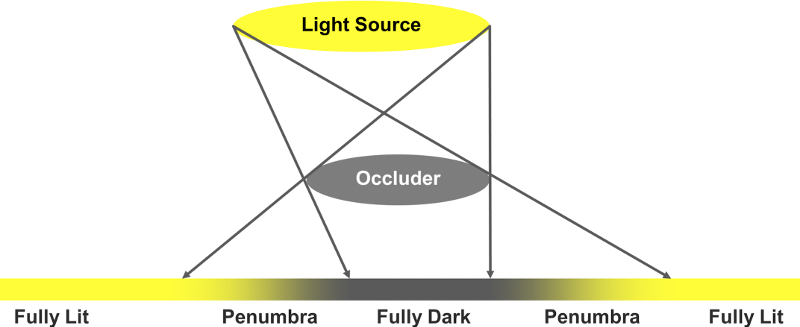
\includegraphics[width=0.65\textwidth]{figures/intro/shadow}
	\caption{软阴影形成的机制,由于光源具有一定的面积,使其包含完全遮挡,部分遮挡及完全光照三个区域(图片来自PowderVR)}
	\label{f:intro-shadow}
\end{figure}




\paragraph{环境遮挡}
对于更大面积的环境光(ambient light)\myindex{环境光}{ambient Light},如环境贴图,天空盒,或者来自其他物体反射的间接光照等,其光源往往来自整个半空间,往往不可能通过以上的方式计算物体间的遮挡效果。在早期的光照计算中,人们通常忽略这种阻挡关系,这造成场景中的缝隙等被较多遮挡的地方比实际的效果要明亮,如图\ref{f:intro-ao}(a)所示,这是因为对于这些地方我们并没有考虑它的遮挡关系,这使得整个物体表面会看起来更平坦,缺乏立体感。

\begin{figure}
\begin{fullwidth}
	\begin{subfigure}[b]{0.325\thewidth}
		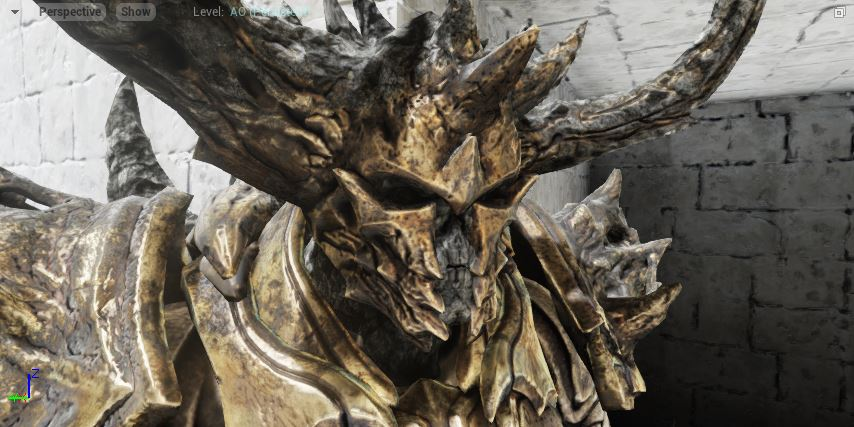
\includegraphics[width=1.\textwidth]{figures/intro/ao-1}
		\caption{不包含AO的场景}
	\end{subfigure}
	\begin{subfigure}[b]{0.325\thewidth}
		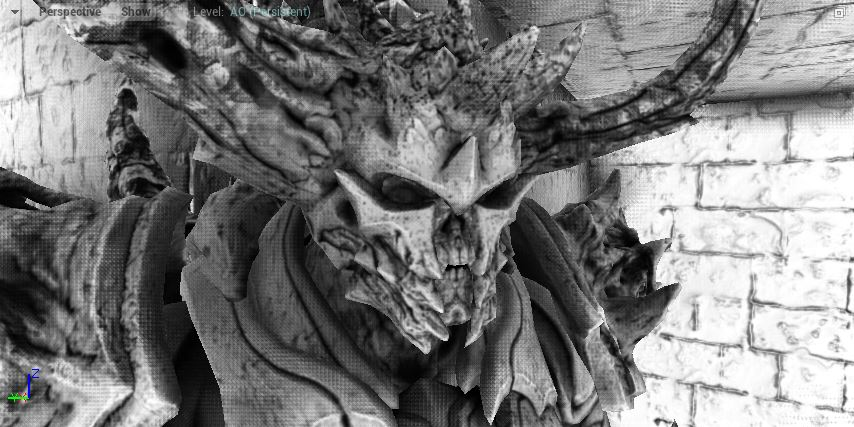
\includegraphics[width=1.\textwidth]{figures/intro/ao-2}
		\caption{仅AO}
	\end{subfigure}
	\begin{subfigure}[b]{0.325\thewidth}
		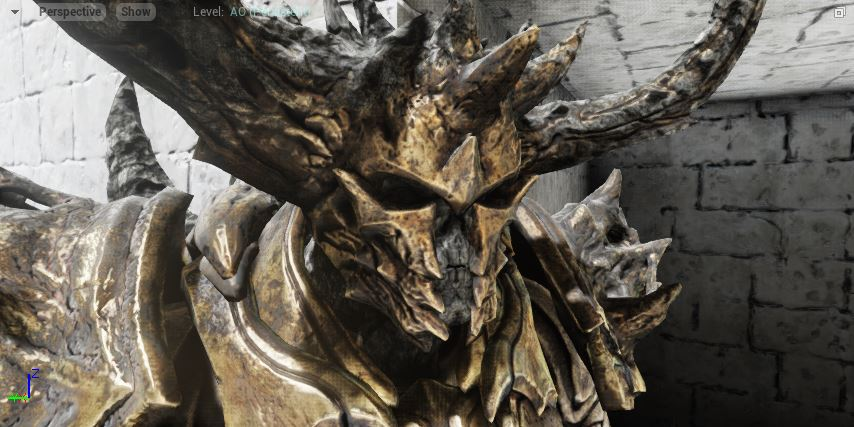
\includegraphics[width=1.\textwidth]{figures/intro/ao-3}
		\caption{包含AO的场景}
	\end{subfigure}
\caption{AO对渲染的影响,注意(c)图中墙砖的裂缝,以及人物颈部等地方由于部分被遮挡显得更暗 (图片来自Unreal Engine 4官方文档)}
\label{f:intro-ao}
\end{fullwidth}
\end{figure}

\cite{a:Shape-from-shadingonacloudyday}首次指出了这种环境阻挡对于图形识别以及增强图像质量的重要性,2010年Hayden Landis, Ken McGaugh和Hilmar Koch因为推进环境遮挡(ambient occlusion,AO)\myindex{环境遮挡}{ambient occlusion}在渲染技术中的运用而获得当年的奥斯卡科学技术奖,之后AO被大量应用于电影工业,如今主流的商业游戏引擎也几乎都支持某种程度(静态或动态)的AO。

AO的计算实际上是要针对每个点,在该点法线对应的半空间上,针对每一个方向对可见性函数(visibility function)进行积分运算,其值为一个介于0到1之间表示遮挡程度的值。对于静态的场景我们可以预计算出这个值;在离线渲染的环境下,可以使用蒙特卡洛方法使用随机抽样的方式求积分\cite{a:GlobalIlluminationandAllThat};而对于实时环境,则需要更高效的方法,例如由CryTek提出的基于屏幕空间的环境遮挡(screen space ambient occlusion,SSAO),以及Unreal Engine 4使用距离场来加速AO的计算。




\paragraph{反~~射}\myindex{反射}{reflection}
光线在物体表面之间穿梭,经过多次反射或折射最后才会进入摄像机,形成图像,如果一个表面是光滑的,或者不是完全粗糙的,则这些表面可以反射它周围的环境,表面越光滑,则其反射的场景越清晰,否则则越模糊。反射几乎无处不在,它是高质量图形渲染不可缺少的部分,如图\ref{f:intro-reflection-1}所示。

\begin{figure}
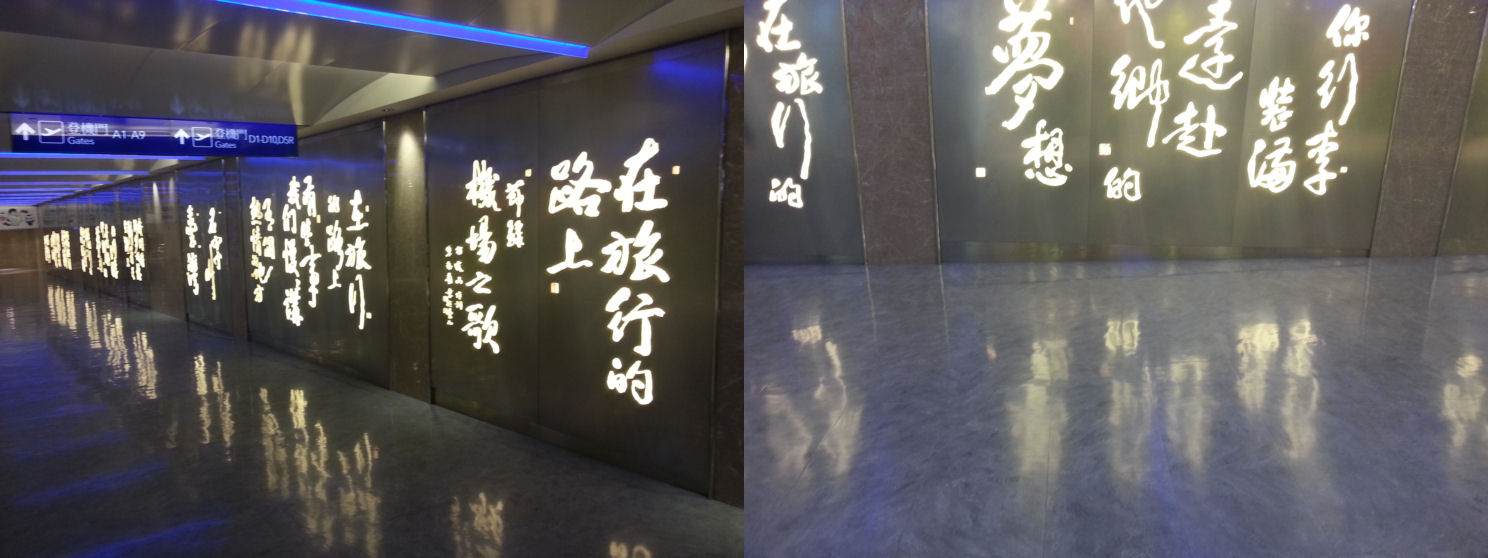
\includegraphics[width=1.\textwidth]{figures/intro/reflection}	
\caption{反射无处不在,较光滑的表面能够比较清晰地反射周围的环境,图为台湾桃园国际机场的走廊}
\label{f:intro-reflection-1}
\end{figure}

反射通常也是使用其他一些近似技术来计算。最经常使用的是基于图像的光照技术(image-based lighting,IBL),这种技术通常将要反射的“环境”渲染为一张图,然后渲染时通过查询这个贴图来计算来自周围的环境光照;对于粗糙的表面可以使用过滤的技术来实现粗糙表面的效果,这种技术大大减少了反射效果的计算时间,本书将在第\ref{chp:prt}介绍基于图像的光照技术。

\begin{figure}
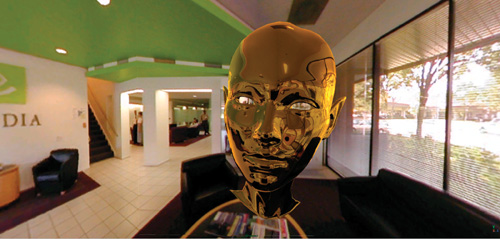
\includegraphics[width=1.\textwidth]{figures/intro/reflection-1}	
\caption{使用基于图像的技术渲染物体对环境的反射,整个周围环境被渲染到一个贴图中,表面着色时直接将这个贴图作为入射光源,其中环境贴图的光照是与观察点的位置无关的}
\label{f:intro-reflection-2}
\end{figure}

对于比较远的环境,可以认为“环境”是和位置无关的,而仅与方向有关。环境贴图可以使用一个放置于场景中心的一个鱼眼镜头的照相机来生成,整个环境被制作成一张立方体贴图(cube map)或者球面贴图(spherical map),如图\ref{f:intro-reflection-2}所示,通常游戏中的天空盒就是一张远距离的环境贴图。




\paragraph{间接光照}\myindex{间接光照}{indirect lighting}
除了上述镜面或光泽反射的光照,环境对于漫反射表面的影响非常重要,它最重要的效果称为颜色渗透\footnote{通过后面第\ref{sec:intro-material-model}节对材质模型的学习,颜色渗透是由于漫反射光从物体内部反射回空中时,被乘以了一个反射率,这个反射率$baseColor$即是物体表面的真实颜色,因此漫反射光携带了物体的颜色,从而能够影响周围的环境。}(color bleeding)\myindex{颜色渗透}{color bleeding},例如一个红色的地毯靠近一侧墙面则会使墙面呈现粉红色,颜色渗透的效果如图\ref{f:intro-indirect}所示。

\begin{figure}
\sidecaption
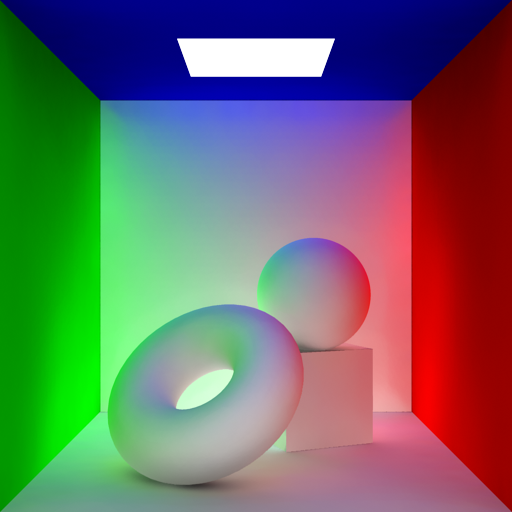
\includegraphics[width=0.45\textwidth]{figures/intro/indirect}	
\caption{环境对漫反射表面的影响,这种效果称之为颜色渗透,这种效果的计算非常昂贵,但是这种效果对于全局光照非常重要}
\label{f:intro-indirect}
\end{figure}

间接漫反射几乎是最重要的全局光照效果,它的计算特别昂贵,其涉及渲染方程针对整个半球空间的积分计算,目前主要的解决方法还是预处理,间接漫反射光照的处理主要有两类方法,一类是基于光照贴图(light map)\myindex{光照贴图}{light map}的方法,这类方法仅针对静态场景,由于漫反射表面向各个方向反射的光照是相同的,因此表面的光照值可以被缓存起来,很多方法可以用来生成光照贴图,例如光线追踪,辐射度方法,辐射照度缓存以及光子映射等方法。

对于动态物体,如角色,移动的交通工具等,常用的处理方法则是在空白空间对环境光照进行稀疏采样,在Unity中这些采样点称为一个光照探针(light probe)\myindex{光照探针}{light probe},如图\ref{f:intro-light-probe}所示,然后在运行时使用插值的方法来计算间接光照。这样做的理由是因为漫反射通常都是低频的,相邻点之间的颜色值变化不大,其间的点的值可以通过插值计算。由于这些采样点是预处理的,所以动态物体并不能影响场景中其他物体,它只能接受来自其他静态环境的影响,这方面可以参见后面第\ref{chp:prt}章的内容。

\begin{figure}
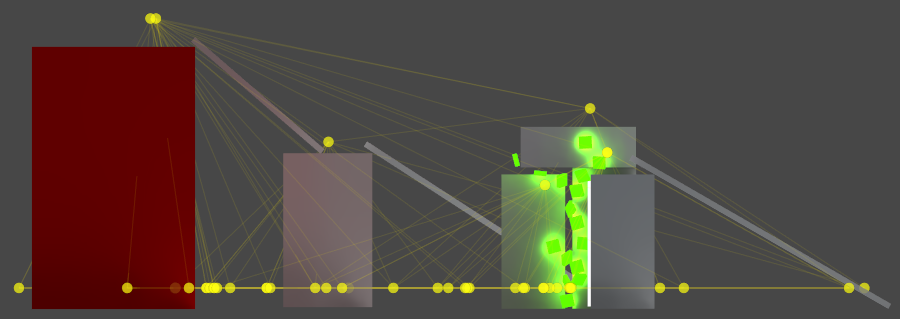
\includegraphics[width=\textwidth]{figures/intro/LightProbes}	
\caption{Unity使用光照探针对环境进行采样,这发生在预处理阶段,在运行时阶段,渲染器从邻近的采样点中取值对其间的点进行插值(图片来自Unity官方文档)}
\label{f:intro-light-probe}
\end{figure}



\paragraph{焦~~散}\myindex{焦散}{caustics}
在全局光照模型中,焦散(caustics)效果尤其明显。广义的焦散是指光从光源出发,经过至少一次光泽反射,最后通过一个光泽或漫反射面 反射后进入摄像机。在计算机图形学中尤其指光通过光泽面的反射或折射后,多束光落在同一个漫反射表面点上(例如由于玻璃或水面等弯曲面使折射后多束光落在桌面上),导致这些点的光照特别明亮,如图\ref{f:intro-caustics}中所示的一些常见焦散的效果。

\begin{figure}
\begin{fullwidth}
	\begin{subfigure}[b]{0.26\thewidth}
		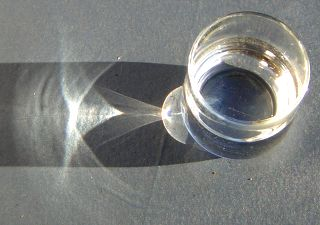
\includegraphics[width=1.\textwidth]{figures/intro/Caustics-1}
	\end{subfigure}
	\begin{subfigure}[b]{0.2758\thewidth}
		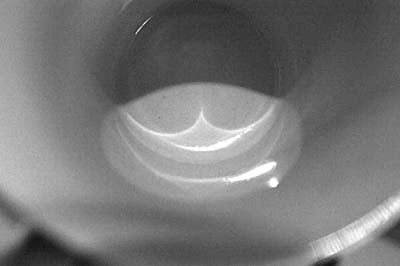
\includegraphics[width=1.\textwidth]{figures/intro/Caustics-2}
	\end{subfigure}	
	\begin{subfigure}[b]{0.19\thewidth}
		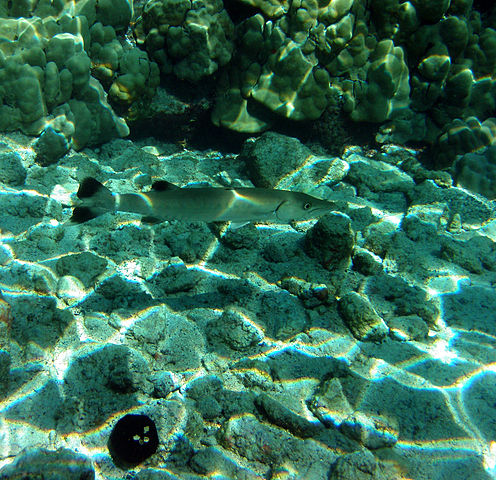
\includegraphics[width=1.\textwidth]{figures/intro/Caustics-3}
	\end{subfigure}	
	\begin{subfigure}[b]{0.246\thewidth}
		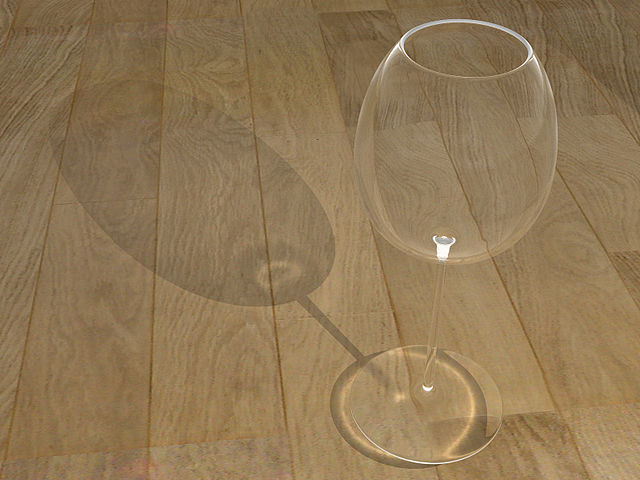
\includegraphics[width=1.\textwidth]{figures/intro/Caustics-4}
	\end{subfigure}
\caption{由于多束光经过反射或折射后落在同一点上,焦散效果在全局光照中特别明显(图片来自Wikipedia)}
\label{f:intro-caustics}
\end{fullwidth}
\end{figure}

对焦散的渲染尤其困难,其主要原因是这样方向光线的采样几率很低,甚至几乎可以认为是零,导致一般的采样方法根本不能获得足够的信息,例如光子映射技术就是使用完全不同于采样的回归方法才能比较好的处理计算焦散。



\paragraph{散~~射}\myindex{散射}{scattering}
到目前为止,所有我们讨论的全局光照现象,都仅限于光与物体表面进行交互。在现实环境中,许多物体部分或全部是半透明的(translucent):即光进入物体表面后,部分被吸收(absorbed),部分发生散射(scattered)最后从物体表面发射出去,其中这个出射点的位置可能和入射点的位置不一样。

由于散射效果的计算相当复杂,因此和其他前面提到的技术一样,计算机图形学中也存在很多近似的方法来处理散射效果。特别地,对于散射的计算,存在两大类方法,它们分别处理散射导致的两种比较明显的子分类效果,即次表面散射和参与介质。

次表面散射(subsurface scattering)\myindex{次表面散射}{subsurface scattering}是散射中最复杂的效果,它表示由于物体内部存在介质的不连续性,导致折射进物体内部的光在经历多次散射之后,重新从另一个位置反射回空中。它要求比较真实地模拟散射效果,并且它处理的都是要求视觉表现比较真实的材料,例如大理石,皮肤,叶子,蜡烛,牛奶等。例如对于皮肤,它有约6\%的光被直接反射,剩下94\%的光被散射,并且散射只发生在表面以下一小部分厚度的空间内,如图\ref{f:intro-sss}所示。

\begin{figure}
\sidecaption
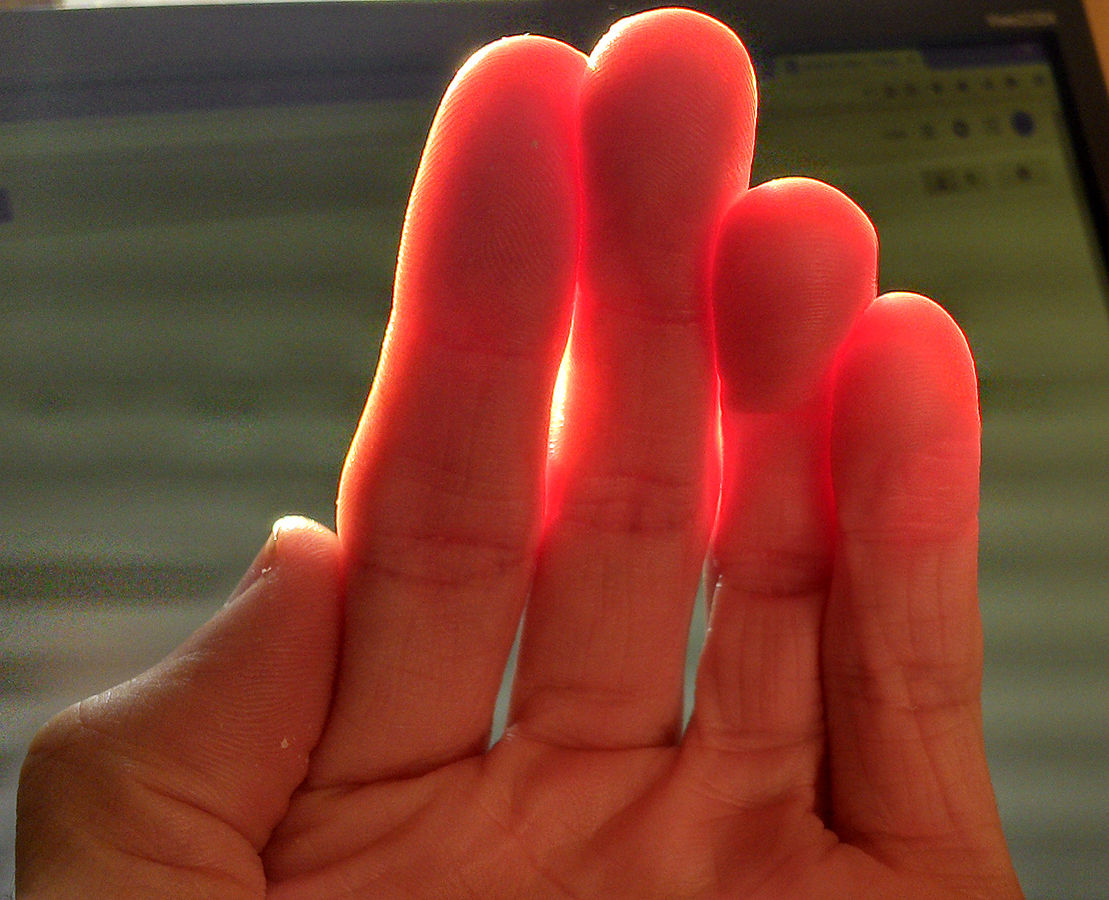
\includegraphics[width=0.5\textwidth]{figures/intro/subsurface-scattering}	
\caption{光可以进入皮肤表面,由于物体内部介质的不连续,在表面以下部分区域内发生多次散射,然后从另一个地方反射回空中}
\label{f:intro-sss}
\end{figure}

关于次表面散射,本章第\ref{sec:intro-bsdf}节会介绍Disney使用的近似然而精确度很高的次表面散射模型,它用在了电影《超能陆战队》中除头发以外的所有次表面散射情形。

参与介质(participating media)\myindex{参与介质}{participating media},例如云,烟,雾等在自然界是普遍存在的,它们也导致了很多有趣的视觉现象。当光在参与介质中传播时,部分被吸收,其他则经过多次散射后从不同的位置离开表面。参与介质与次表面不同的是,次表面往往只是物体表面很浅的一层,而参与介质往往整个内部都是半透明的,光线能够从一边进入,然后从另一边离开。参与介质能够有效地增强环境的氛围,以及对场景深度的感知。

\begin{figure}
	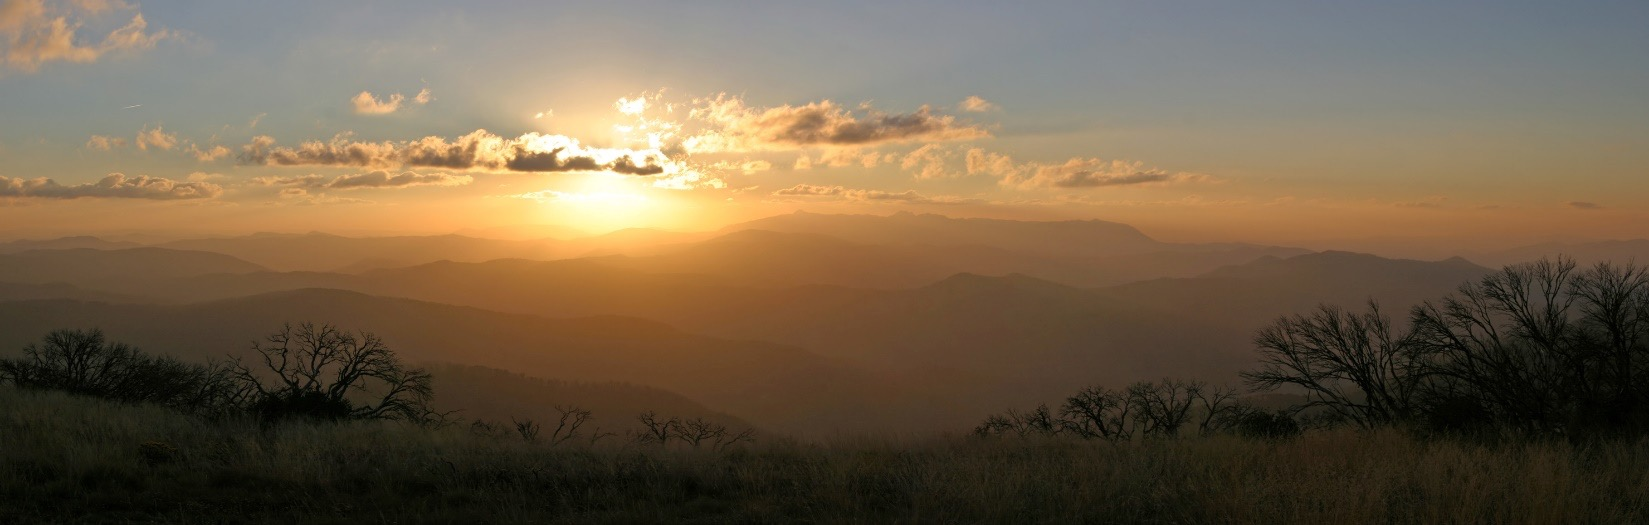
\includegraphics[width=1.0\textwidth]{figures/intro/Participating-media}
	\caption{参与介质在大自然中无处不在,例如云层,空气,烟雾等,并且对整个环境的光照有非常大的影响}
	\label{f:intro-Participating-media}
\end{figure}

本书将在第\ref{chp:pm}章介绍一些参与介质的渲染技术。





\section{辐射度量学}
光学中关于光的测量这一分支,称为辐射度量学(radiometry)\myindex{辐射度量学}{radiometry}。\cite{a:TheRenderingEquation}首次将辐射度量学引入到计算机图形学中,用于测量和计算计算机图形学中光的传播,并由此推导出渲染方程(the rendering equation)\myindex{渲染方程}{the rendering equation}。渲染方程保留了辐射度量学两个最基本的特性即赫姆霍兹互反律(Helmholtz reciprocity)\myindex{赫姆霍兹互反律}{Helmholtz reciprocity}和能量守恒(energy conservation)\myindex{能量守恒}{energy conservation},现代图形学理论基于渲染方程提出了大量的模型用于简化和加速渲染方程的计算,在这两个基本物理特征的保障下,这些模型能够达到非常真实的图形品质。

辐射度量学定义了一组基本的物理量用来测量光辐射,因此这些度量也成为计算机图形学中最重要的基本概念,这几个度量的名称及单位如表 \ref{t:radiometric-quantities}所示。

\begin{table}
\caption{辐射度量学中的基本度量,这些度量也成为渲染方程的基本度量}
\label{t:radiometric-quantities}

\begin{tabular}{p{0.3\textwidth}|p{0.3\textwidth}|p{0.2\textwidth}|p{0.15\textwidth}}
\hline
   中文名称&英文名称&单位&符号  \\
  \hline
  辐射能量&radiant energy & $J$& $Q$\\
  辐射通量&radiant flux & $W$  & $\Phi$\\
  辐射照度&irradiance & $W/m^2$ & $E$\\
  辐射强度&radiant intensity & $W/sr$ & $I$\\
  辐射亮度&radiance & $W/(m^2\cdot sr)$& $L$\\
\hline
\end{tabular}
\end{table}

在开始讨论这些度量之前,必须首先了解立体角(solid angle)\myindex{立体角}{Solid Angle}的概念,如图\ref{f:intro-solid-angle}所示。在几何学中,立体角是2D角度的概念在3D空间的延伸,它表示在3D空间,从某个点观察,另外一个物体有多“大”。立体角的数学符号通常用$\Omega$表示,其单位为$sr$,它是球面度(steradians)\myindex{球面度}{steradians}的缩写。立体角也可以理解为3D空间中以某一点为起点的多个方向的集合。

\begin{figure}
\sidecaption
	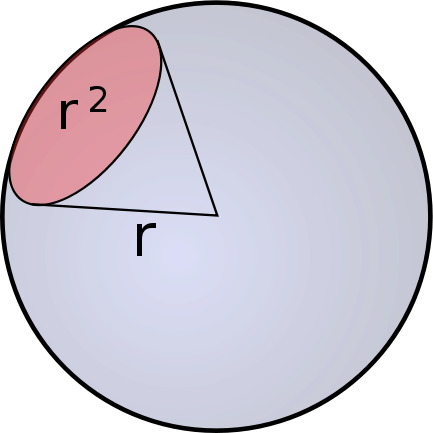
\includegraphics[width=0.35\textwidth]{figures/intro/solid-angle}
	\caption{立体角的概念,它表示单位球体上一块区域对应的球面部分的面积。根据立体角的定义,如果球面上任意一块区域的面积等于球半径的平方,当从球心观察时,该区域面积就是$1sr$}
	\label{f:intro-solid-angle}
\end{figure}

正如在2D中,使用单位圆上的一段弧线的长度来表示其对应“角度”的大小,在3D中,使用单位球体上一块区域面积的大小来表示其对应的“立体角”的大小。所以一个物体相对于某一点的立体角的大小,等于这个物体投影到以该点为球心的单位球体上的面积。

根据上述立体角的定义,如果球面上任意一块区域的面积等于球半径的平方,当从球心观察时,该区域面积就是$1sr$。

在球面坐标系中,单位球体上任意一块区域$A$的面积可以简单地表示为:

\begin{equation}
	\Omega= {\rm \iint}_A \sin\theta {\rm d}\theta {\rm d}\varphi
\end{equation}

\noindent 其中,$\theta$表示经度,$\varphi$表示纬度,所以整个球面的立体角为$4\pi$,对于一个正方体的一个面,从该正方体的中心点测量的立体角为$ \cfrac{2}{3}\pi$。




\subsection{辐射能量}
在辐射度量学中,最基本的单位是辐射能量(radiant energy)\myindex{辐射能量}{radiant energy},表示为$Q$,单位为J(焦耳),辐射能$Q$是以辐射的形式发射,传播或接收的能量。每个光子都携带一定的能量,这个能量正比于它的频率$v$,即:

\begin{equation}
	Q=hv
\end{equation}

\noindent 其中,$h=6.62620\times 10^{-34} J\cdot s$为普朗克常数(Planck constant)\myindex{普朗克常数}{Planck constant}。光子的频率(或者说能量)影响着光子与物体表面的交互,更重要的是,它影响着光与感应器(例如人眼中的视锥细胞和视杆细胞)之间的作用,使不同频率的光被察觉为不同的颜色。在可见光谱(visible spectrum)\myindex{可见光谱}{visible spectrum}中,更“蓝”的光子具有更高的能量,而更“红”的光子具有更低的能量。 




\subsection{辐射通量}
辐射通量(radiant flux)\myindex{辐射通量}{radiant flux}记为$\Phi$,表示光源每秒钟发射的功率(${\rm d}Q/{\rm d}t$),其单位为瓦特(watt)$W$,例如一个灯泡可能发射100瓦特的辐射通量。在辐射测量中,都是基于这个辐射通量来测试能量,而不是使用总的能量$Q$,所以以下这些度量都是在单位时间(每秒)下发生的。





\subsection{辐射亮度}
在辐射度量学中,基本上考虑的是从面$A$的一部分射出的光能量。这个面可能是虚构的,也可能就是光源的真实的辐射面,或固体的一个受照面。如果固体是不透明的,则考虑的是反射光;如果固体是透明或半透明的(这时有一部分光被吸收或散射),通常测量的是透射光。

\begin{figure}
\sidecaption
	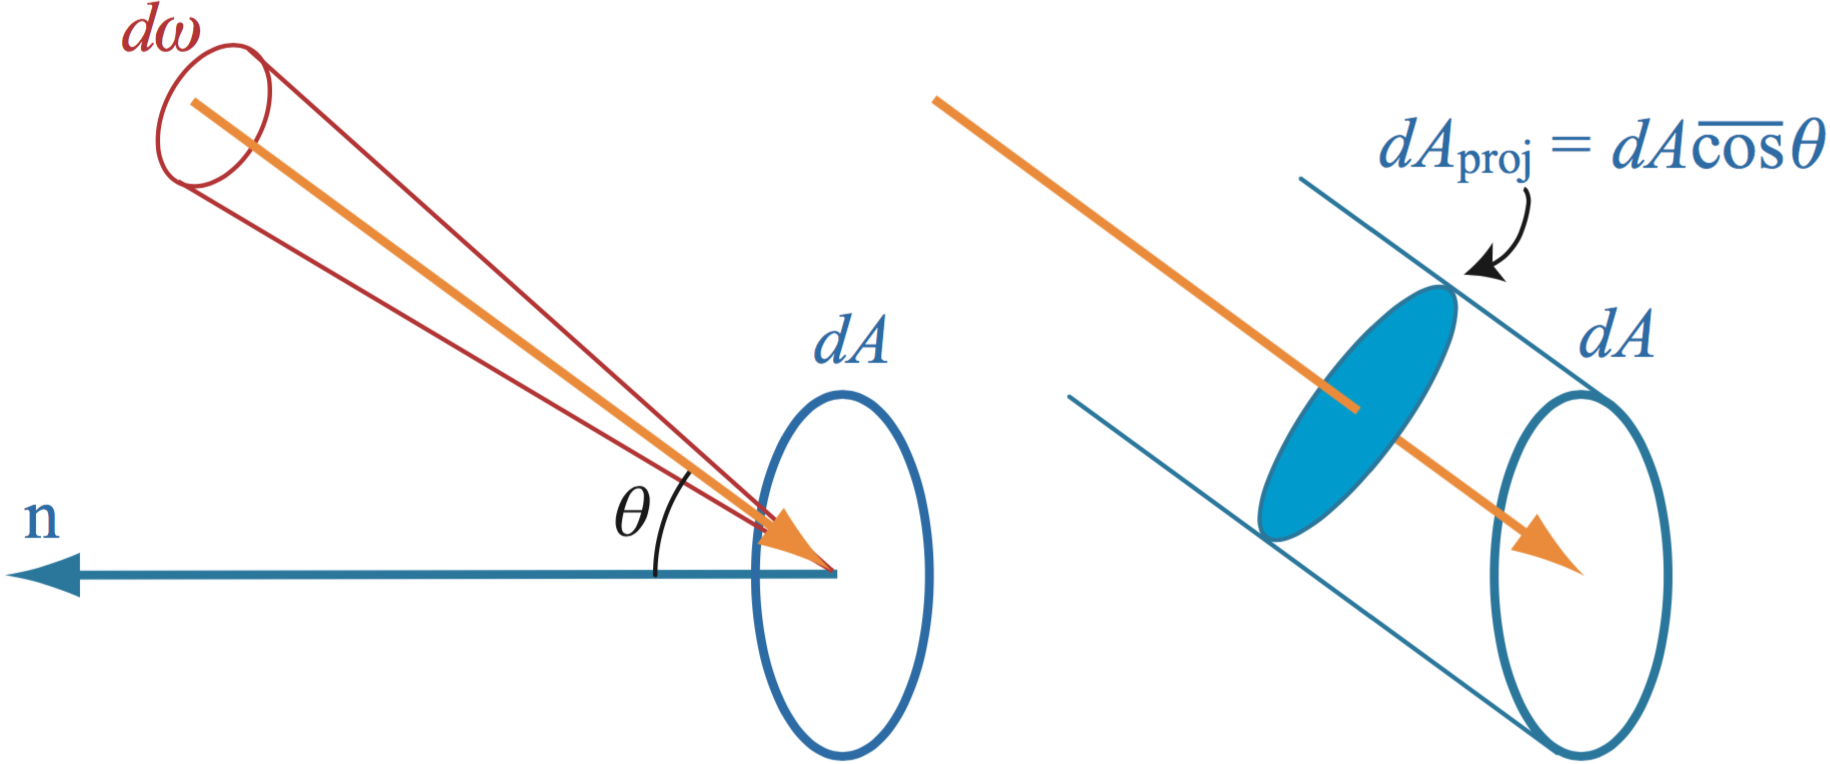
\includegraphics[width=0.65\textwidth]{figures/intro/radiance}
	\caption{辐射亮度表示的是某个点在某个方向上的亮度,在计算机图形学中它是一束光的亮度,是渲染方程最终要计算的量}
	\label{f:intro-radiance}
\end{figure}

设$P(\xi,\eta)$是$A$面上的一个点,以面上任意一组方便的曲线为参考坐标。现在在$P$点取一面元${\rm d}A$ ,并围绕极角$(\alpha,\beta)$方向取一立体角${\rm d}\omega$,另外设${\rm d}\omega$方向与${\rm d}A$ 法线的夹角为$\theta$,如图\ref{f:intro-radiance}所示,则在单位时间内由面元${\rm d}A$ 发射到${\rm d}\omega$内的能量(时间平均)值${\rm d}\Phi$可以表示为:

\begin{equation}\label{eq:intro-energy}
	{\rm d}\Phi=L\overline{\cos}\theta {\rm d}A {\rm d}\omega
\end{equation}

\noindent 其中,$L$是一个因子,一般与位置$(\xi,\eta)$和方向$(\alpha,\beta)$有关,即:

\begin{equation}
	L=L(\xi,\eta;\alpha,\beta)
\end{equation}

\noindent 式中引入因子$\cos\theta$,是因为物理上有意义的量是${\rm d}A$在垂直于$(\alpha,\beta)$方向的平面上的投影,而非${\rm d}A$本身。$\overline{\cos}$表示$\cos\theta$的最小值为$0$,这是因为光不能向该面的背面发射。$L$称作点$(\xi,\eta)$处方向$(\alpha,\beta)$上的辐射亮度(radiance)\myindex{辐射亮度}{radiance},其单位为$W/(m^2\cdot sr)$。

辐射亮度测试的是单束光的量度,它也正是感应器(例如人的眼睛,或者场景中的虚拟摄像机)测量的度量,所以它在光照计算中特别重要。计算渲染方程的目标就是计算出表面上的点到摄像机所在方向上的辐射亮度。另外值得注意的是,$L$的值不随距离发射点距离的变化而变化。

通常用两种不同的方式把${\rm d}\Phi$分解为两个量的乘积,以表示它对${\rm d}\omega$和${\rm d} A$的显式关系:

\begin{equation}\label{eq:intro-energy-1}
	{\rm d}\Phi={\rm d}I {\rm d}\omega={\rm d}E {\rm d}A
\end{equation}

\noindent 在接下来的两小节将分别讲述这两个新的度量$I$和$E$。





\subsection{辐射强度}
比较方程\ref{eq:intro-energy}和\ref{eq:intro-energy-1}两式,可以得出:

\begin{equation}
	{\rm d}I= \cfrac{{\rm d}\Phi}{{\rm d}\omega}=L\overline{\cos}\theta {\rm d}A
\end{equation}

\noindent 对一个面$A$的区域求积分得到:

\begin{equation}\label{eq:intro-radiant-intensity}
	I(\alpha,\beta)={\rm \int} L\overline{\cos}\theta {\rm d}A
\end{equation}

$I$称为面积$A$在方向$(\alpha,\beta)$上的辐射强度(radiance intensity)\myindex{辐射强度}{radiance intensity},其单位为$W/sr$。$I$也是一个与距离无关的量,但它是与发射面$A$的面积有关的,由于光源通常具有一定的形状和面积,所以图形学中常常使用$I$来表示一个光源的辐射强度分布,这个分布是方向的函数,如图\ref{f:intro-radiant-intensity}表示一个点光源,这个点光源每秒发出100瓦特的辐射通量,但是它在不同的方向上具有不同辐射强度。

\begin{figure}
\sidecaption
	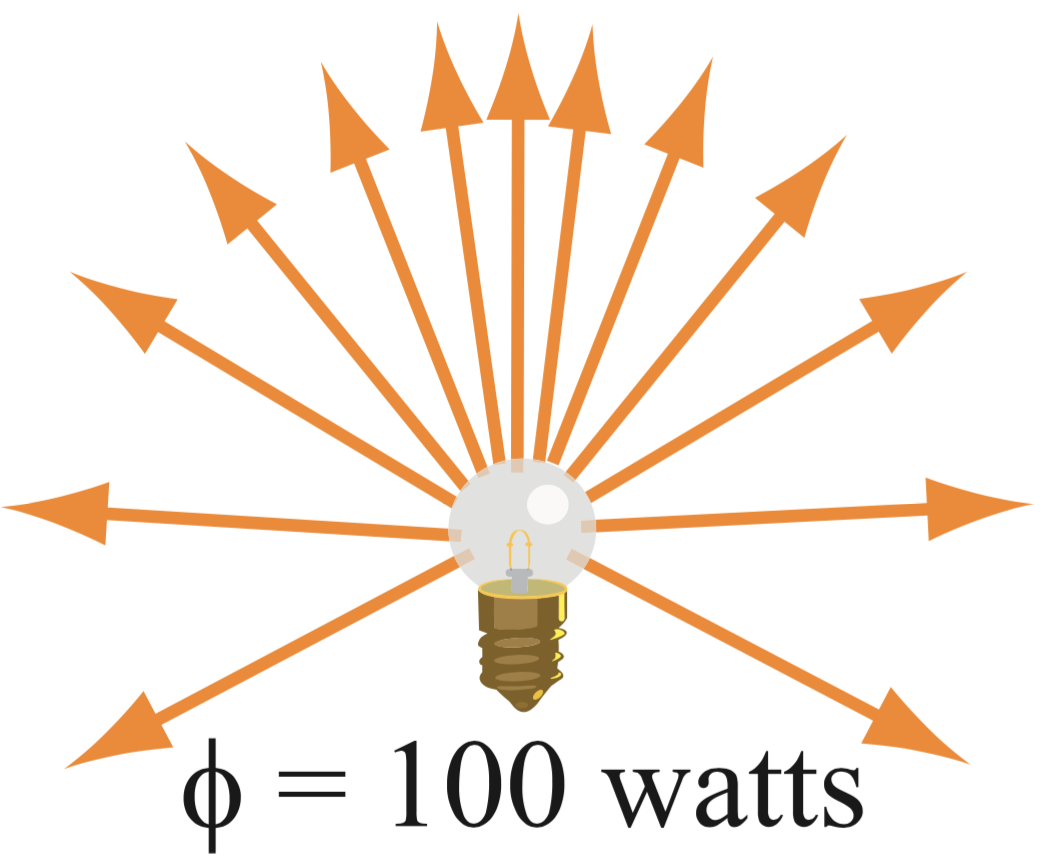
\includegraphics[width=0.35\textwidth]{figures/intro/radiant-intensity}
	\caption{一个灯泡在不同的方向上可能具有不同的辐射强度,辐射强度也是计算机图形学中表示各种光源光照的度量}
	\label{f:intro-radiant-intensity}
\end{figure}

当发生反射时,$L$随方向的变化取决于这个面的性质,特别取决于它是粗糙的还是光滑的,它是自发光还是反射或透射别的光。常常允许假设,在很好的近似下,$L$与方向无关,这时辐射称为是各向同性的(isotropic)\myindex{向同性的}{isotropic}。如果辐射是各向同性的,并且辐射面是平面,则方程\ref{eq:intro-radiant-intensity}简化为:

\begin{equation}\label{eq:intro-radiant-intensity-1}
	I(\alpha,\beta)=I_0 \overline{\cos}\theta 
\end{equation}

\noindent 其中

\begin{equation}
	I_0={\rm \int} L{\rm d}A
\end{equation}

这时,任何方向上的辐射强度随该方向与面法线间夹角的余弦的变化而变化。公式\ref{eq:intro-radiant-intensity-1}通常称为朗伯余弦定理(Lambert's cosine law)\myindex{朗伯余弦定理}{Lambert's cosine Law},如图\ref{f:intro-lambert-cosine-law}所示。此时,如果是发射面,则称为漫发射;如果是反射面,则称为漫反射。如果一个辐射源其表面辐射亮度不随方向变化,则称为朗伯体。

\begin{figure}
\sidecaption
	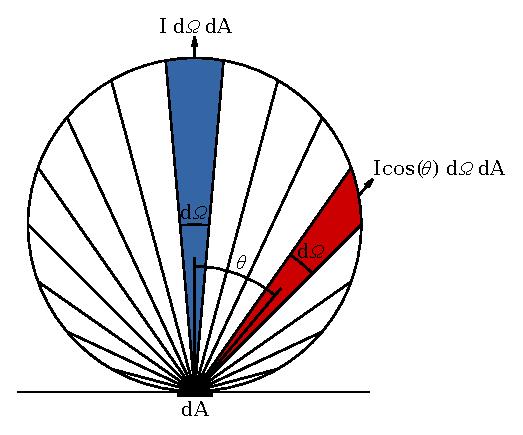
\includegraphics[width=0.6\textwidth]{figures/intro/Lambert_Cosine_Law}
	\caption{在一个漫反(发)射面,法线方向和非法线方向的每秒光子发射情况。每个楔形区域内光子的发射量正比于它们的面积}
	\label{f:intro-lambert-cosine-law}
\end{figure}





\subsection{辐射照度}\label{sec:irradiance}
同理,比较方程\ref{eq:intro-energy}和\ref{eq:intro-energy-1}两式,可以得出:

\begin{equation}
	{\rm d}E= \cfrac{{\rm d}\Phi}{{\rm d}A}=L\overline{\cos}\theta {\rm d}\omega
\end{equation}

\noindent 而对某一立体角取积分得:

\begin{equation}
	E(\xi,\eta)={\rm \int} L\overline{\cos}\theta {\rm d}\omega
\end{equation}

$E$称为点$(\xi,\eta)$的辐射照度(irradiance)\myindex{辐射照度}{irradiance},其单位为$W/m^2$,它是点$(\xi,\eta)$沿各个方向对辐射亮度$L$的积分,如图\ref{f:intro-irradiance}所示。值得注意的是,前面提到过,在辐射度量学中,基本上考虑的是从面的一部分射出或者接收能量,所以辐射照度虽然表述的是面上一个点的度量,但它实际上是通过该点所在的单位面积来测量的,因为辐射量度$L$也是通过单位面积来测量的。

\begin{figure}
\sidecaption
	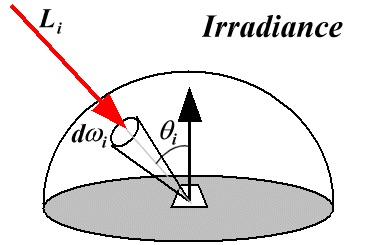
\includegraphics[width=0.45\textwidth]{figures/intro/irradiance}
	\caption{一个面上某点接收来自各个方向的辐射亮度形成辐射照度}
	\label{f:intro-irradiance}
\end{figure}

由于辐射照度表示一个点接收的来自各个方向的辐射亮度,所以在计算机图形学中,它被用来表述表面的一个点接收的所有光照。而渲染方程所要处理的正是通过反射定律及后面要讲述的其他理论,计算出沿某个观察方向的出射亮度$L_o$,通常$L_o$是与入射方向有关的,但是对于漫反射表面,它沿各个方向反射的光照是相同的,所有入射光照的积分就可以被单独计算出来,因此辐射照度是漫反射表面的重要度量,实际上光照贴图(light map)\myindex{光照贴图中}{light map}中存储的正是辐射照度值,这方面的知识将在第\ref{chp:prt}章介绍。

辐射照度被用来测量光进入一个表面(更确切地讲一个单位面积)的强度,它也可以表示光离开一个表面的强度,称为出射度,用$M$表示,其也称为辐射度(radiosity)\myindex{辐射度}{radiosity}或者辐射出射度(radiant exitance)\myindex{辐射出射度}{radiant exitance},例如表示一个光源的出射度,或者在辐射度理论(第\ref{chp:rad}章)中首先将整个场景栅格化为多个面片,将每个面片视作一个光源,然后计算出每个面片的出射度。通常用辐射通量密度(radiant flux density)\myindex{辐射通量密度}{radiant flux density}来统称一个表面出射或者入射的强度。

在图\ref{f:intro-directional-irradiance}所示的平行光中,光源的辐射强度是不随表面到光源的距离发生变化的。但是现实世界中大多数光源(例如本章后面将要讨论的点光源和聚光灯等)都不是平行光,那么一般光源的辐射强度是怎样分布的呢?

\begin{figure}
\sidecaption
	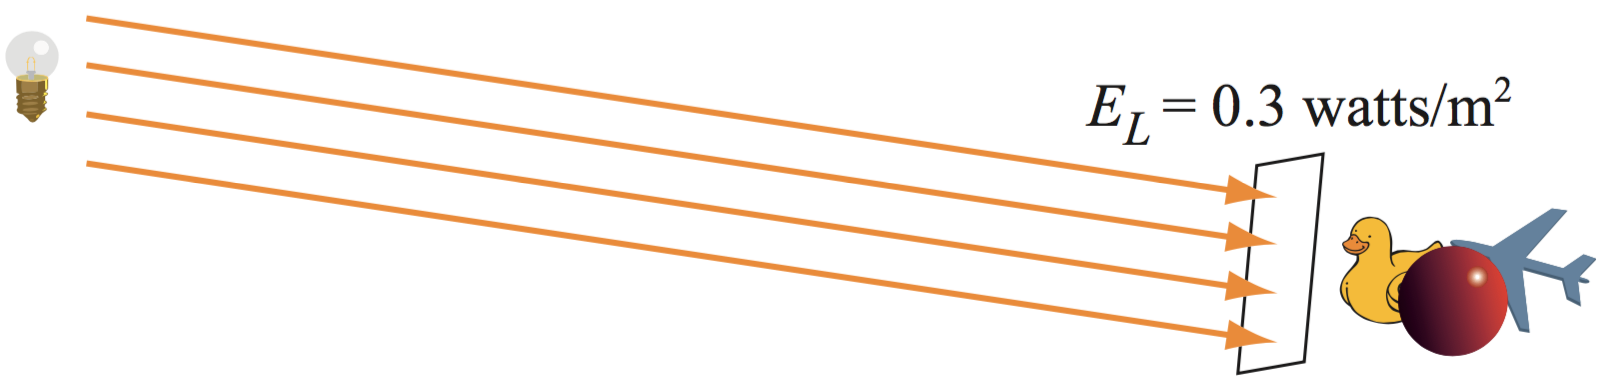
\includegraphics[width=0.65\textwidth]{figures/intro/directional-irradiance}
	\caption{平行光源的出射度不随表面到光源的距离变化而变化}
	\label{f:intro-directional-irradiance}
\end{figure}

如图\ref{f:intro-inverse-square-law}所示,设${\rm d}A$是点$P$处的面元,$QP=r$,又设$\theta$是$QP$与${\rm d}A$的法线夹角,则光源在单位时间内射过${\rm d}A$的能量是$I{\rm d}\omega$,其中$I$是光源沿$QP$方向的辐射强度,${\rm d}\omega$是对$Q$所张的立体角。由几何基础学:

\begin{equation}
	\cos\theta {\rm d}S=r^{2}{\rm d}\omega
\end{equation}


\noindent 由此,利用公式\ref{eq:intro-energy-1}即可得出:

\begin{equation}\label{eq:intro-inverse-square-law}
	E= \cfrac{I\cos\theta}{r^{2}}
\end{equation}

公式\ref{eq:intro-inverse-square-law}就是辐射度量学的基本方程,它表达了所谓的照度余弦定律($E$与$\cos\theta$成正比),以及平方反比定律 ($E$与$r^{2}$成反比)。

\begin{figure}
\sidecaption
	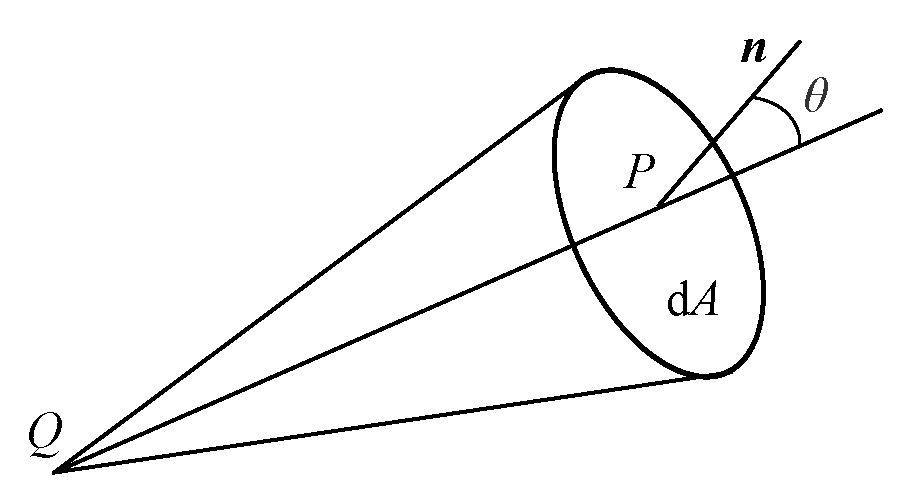
\includegraphics[width=0.5\textwidth]{figures/intro/inverse-square-law}
	\caption{点光源产生的辐射照度}
	\label{f:intro-inverse-square-law}
\end{figure}

由于$E$表示的是一个表面接收周围所有光源(包括直接光源和间接光源)的辐射照度,所以根据平方反比定律可以看出,一个光源距离该表面越远,则其光照贡献越小。









\section{物体的表面着色}
在了解了全局光照应该实现各种物理现象,以及模拟自然光照计算需要的一些基本物理度量之后,从本节开始,我们将开始进入计算机图形学的世界。

正如前言所述,本书除了介绍计算机图形学的一些基本理论知识,另一个重要的目标是试图解释清楚这些理论知识之间的逻辑联系,本节的目标是在没有涉及具体的全局光照方法之前,尝试解释光与物体的交互过程,以及最终怎样被渲染成图像。在本节的末尾,我们仍然会通过这种高层抽象的物体表面着色需求(而不是从基础的数学公式),推导出渲染方程的表达式。然后在第\ref{sec:intro-the-rendering-equation}节,将会更详细地解释渲染方程。




\subsection{几何光学模型} 
本节首先介绍光的一些基础物理特征,这些特征是我们模拟真实的光与物体交互的基础,从而能够渲染出更真实的图像。

在电磁学中,有两种模型用于研究光的性质,第一种为物理光学,第二种为几何光学。物理光学(physical optics)\myindex{物理光学}{physical optics},又称为波动光学(wave optics)\myindex{波动光学}{wave optics},它认为光在介质中以波的形式传播,这种模型可以解释光的衍射和干涉等现象。然而它以光的波长为测量尺寸,这大大超出了计算机图形学的需求。

由于可见光的波长非常短,另一种模型忽略光的波长,即相当于$\lambda\to 0$的极限情况,并证明\footnote{感兴趣的读者可以参考书籍\cite{b:PrinciplesofOptics}第三章的推导。}在这种近似处理下,光学定律可以用几何学的语言来描述,这种模型称为几何光学(geometric optics)\myindex{几何光学}{geometric optics},或者称为光线光学(ray optics)\myindex{光线光学}{ray optics},因为这种模型下能量可以看作是沿着直线传输。几何光学模型正是被计算机图形学广泛采用的模型。

当然,几何光学模型仍然比较复杂,在计算机图形学中,我们作出了一些简化假设,这虽然限制了一些效果如衍射,但是它处理起来相对简单,并且满足一般图形学的需求。这些假设包括:

\begin{itemize}
	\item 物体的表面是绝对光滑\footnote{当然现实世界的物体表面不是绝对光滑的,但是这种粗糙度介于光的波长和一个像素的尺寸之间,这种粗糙度可以通过下一节介绍的微面元技术实现,它本质上是反射和折射的一种聚合。}(smooth)的。
	\item 光仅可以被发射(emitted),反射(reflected)或者传播(transmitted)。
	\item 光以无限快的速度沿直线传播。
\end{itemize} 

在这些假设下,光的反射由反射定律(law of reflection)\myindex{反射定律}{law of reflection}决定,即: 给定一条入射光线$\mathbf{l}$和表面法线$\mathbf{n}$,反射光和入射光处于同一个平面, 并且反射光与法线之间的夹角大小等于入射光与法线的夹角大小,如图\ref{f:intro-Ray-optics-model}所示。

\begin{figure}
\sidecaption
	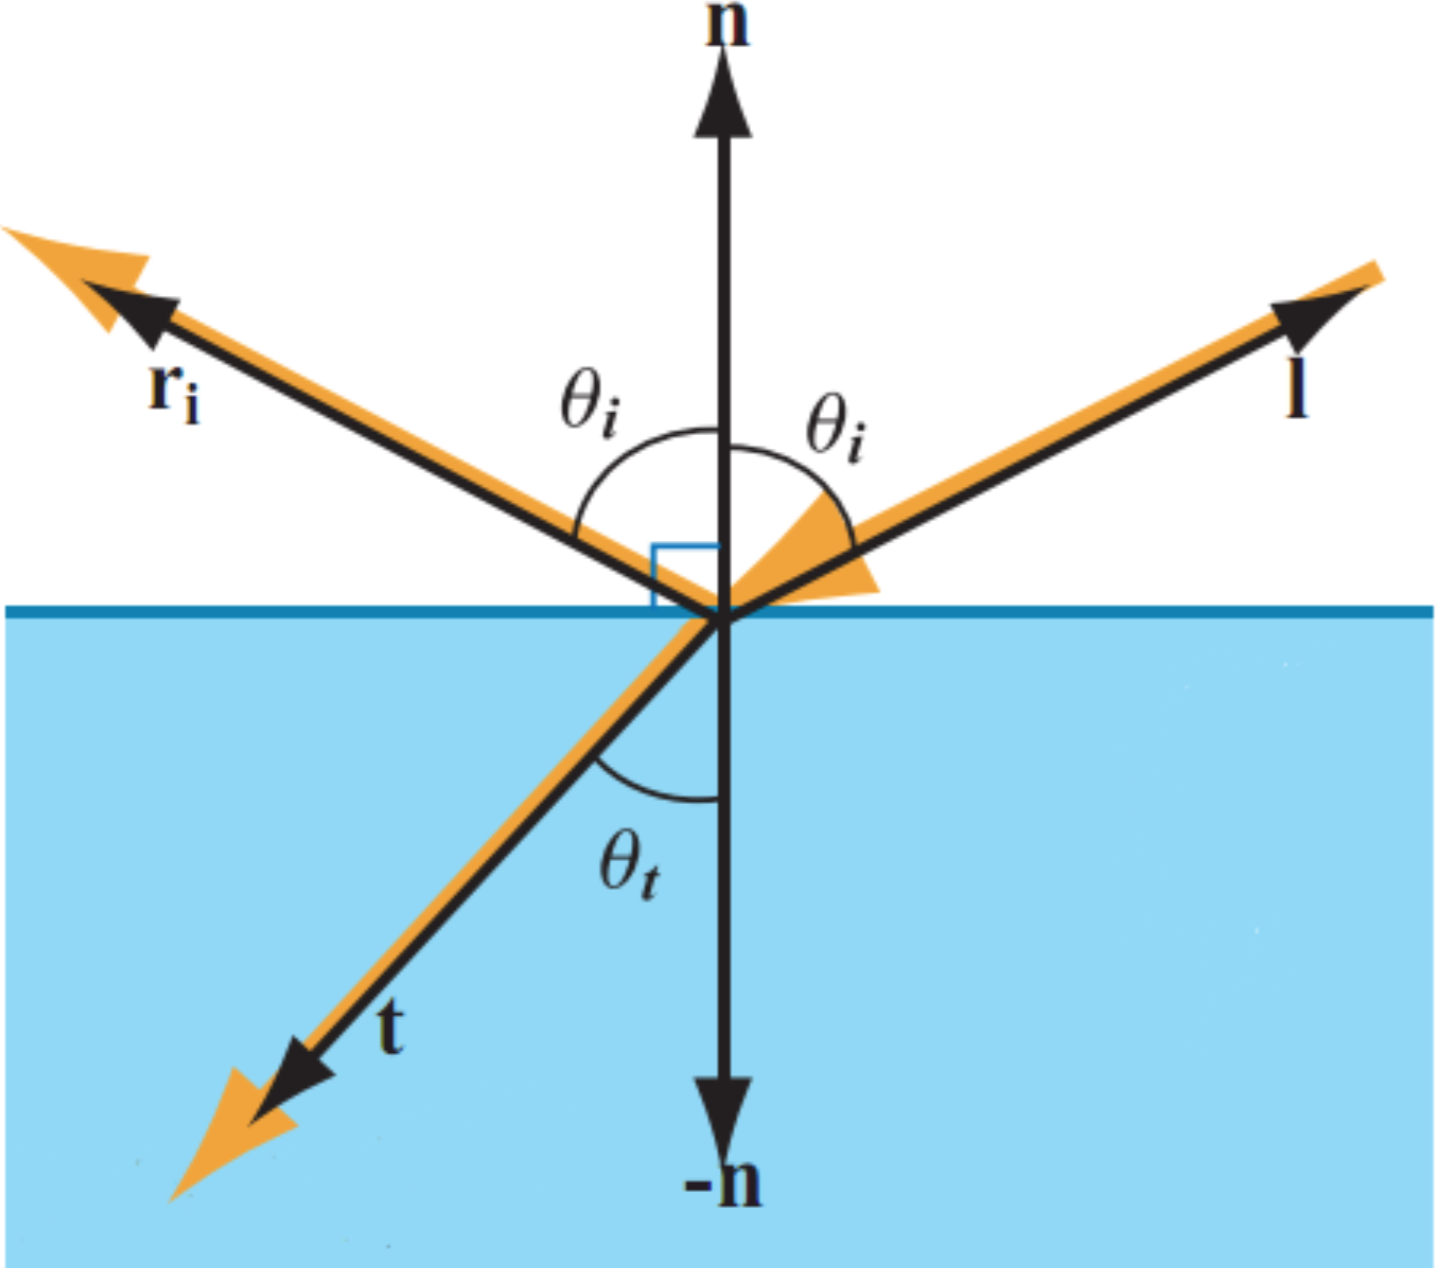
\includegraphics[width=0.4\textwidth]{graphics/gi/ray-optics-1}
	\caption{在几何光学模型中,反射定律和斯涅尔定律决定光的反射和折射}
	\label{f:intro-Ray-optics-model}
\end{figure}

当光在传输过程中,介质的折射率(index of refraction)\myindex{折射率}{index of refraction}发生变化,则会发生折射(refraction)\myindex{折射}{refraction}。当入射光$\mathbf{l}$从具有折射率为$n_1$的介质进入折射率为$n_2$的介质时, 其光线传输方向的偏离$\mathbf{t}$由斯涅尔定律(Snell's law)\myindex{斯涅尔定律}{Snell's law}决定,如图\ref{f:intro-Ray-optics-model}所示,即有:

\begin{equation}\label{eq:intro-snell-Law}
	n_1\sin\theta_1 = n_2\sin\theta_2\ 	
\end{equation}





\subsection{光与表面的交互}
为了模拟光学现象以生成真实的数字图像,我们需要构建一套系统,将几何光学模型应用到计算机图形学中。这套系统定义了在图形渲染过程中,光与表面及其他物体的交互。

这个系统工作的过程可以描述如下:

\begin{enumerate}
	\item 光从光源(例如太阳或其他光源)或其他发光体中发射出来。
	\item 光与场景中的物体进行交互,部分被反射,部分被吸收并可能经过一定路径传播后沿其他方向从物体表面散射出来。
	\item 最后,光被感应器(例如摄像机或者人的眼睛)吸收,形成图像。
\end{enumerate}

这个过程涉及三个组件:光源,材质以及摄像机。在接下来的小节中我们将讨论这些组件,以及它们怎样被用在渲染管线中用于渲染图形。




\subsubsection{光~~源}\label{sec:intro-light-sources}
光源(light sources)\myindex{光源}{light sources}发出光并照亮整个场景,此外,在计算机图形学中,光源一般不会反射或吸收其他光照。

现实世界中的光源是很复杂的,它可能沿不同的方向以及光源表面上的不同位置具有不同的分布,在图形学中一般仅使用少数几种简单的光源模型,这几种模型都假设光源的光照分布只随方向而发生变化。这几种模型包括:

\begin{itemize}
	\item 平行光(directional light)\myindex{平行光}{directional light}:平行光模拟光从无限远的地方发射,这意味着所有由它产生的阴影光线都是平行的,因此这种模型是模拟太阳光的理想选择。
	\item 点光源(point light)\myindex{点光源}{point light}:点光源从一个点向四面八方发出光线,它可以用于模拟如现实世界中的钨丝灯泡发出的光。
	\item 聚光灯(spot light)\myindex{聚光灯}{spot light}:聚光灯限制点光源发出光线的方向,它通常使用两个圆锥体作为参数,其中内部圆锥体的半径内发出的光线最强,从内部到外部圆锥体半径内光线强度逐渐减至零。
\end{itemize}

以上这些光源发出的光线会在场景中像自然光一样进行传播,即这些光线通过最近点测试计算出光线与哪个物体表面的哪个位置相交,然后根据物体表面的材质属性进行着色计算。除此之外,出于性能考虑,场景中还有另外一些(通常是间接)光不会通过这种方式计算,例如大面积的环境光通常通过贴图的方式计算,这包括天空盒(sky light)\myindex{天空盒}{sky light}以及其他环境光照;而低频率的间接漫反射的光可以通过使用低阶的球谐函数近似表述,然后在GPU中使用快速的卷积(convolution)\myindex{卷积}{convolution}计算。

对于直接光源,另一个我们最关心的问题是这个光源的光照用什么物理量表示,以及这个物理量怎样参与到光与表面的交互计算之中。

首先,虽然眼睛等感应器接收的是辐射亮度$L$,但这是一个五维(三个维度表示位置,两个维度表示方向)的量,太过于复杂,所以在图形学中一般不会直接表示光源的辐射亮度分布。考虑到图形学中大部分直接光源的亮度分布都是只与方向有关,所以辐射强度$I$通常用来表示本节提到的几种直接光源的辐射亮度分布。

当然这个方向分布函数不宜太复杂,一般引擎不允许定义具有任意方向分布的光源,例如点光源可能所有方向的辐射强度都相同,聚光灯也是沿着一个圆锥体向外递减。在Unreal Engine 4中,可以对点光源和聚光灯使用一个称为IES\cite{m:IESLightProfiles} 的光源配置(light profiles)\myindex{光源配置}{Light Profiles}的配置文件。IES光源配置文件可以以曲线的方式定义光源的光照强度分布,如图\ref{f:intro-ies}所示。

\begin{figure}
\begin{fullwidth}
	\begin{subfigure}[b]{0.209\thewidth}
		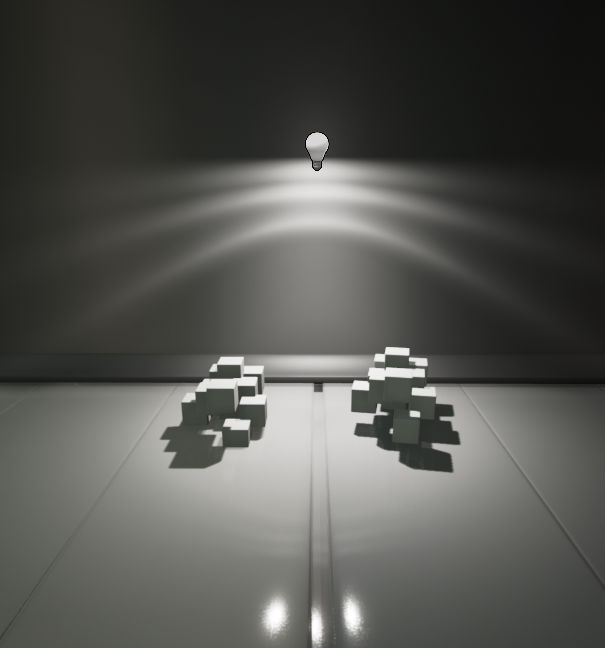
\includegraphics[width=1.\textwidth]{figures/intro/IES_01}
	\end{subfigure}
	\begin{subfigure}[b]{0.213\thewidth}
		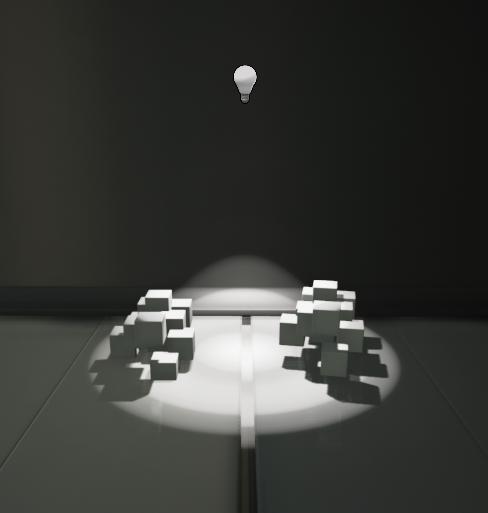
\includegraphics[width=1.\textwidth]{figures/intro/IES_02}
	\end{subfigure}
	\begin{subfigure}[b]{0.247\thewidth}
		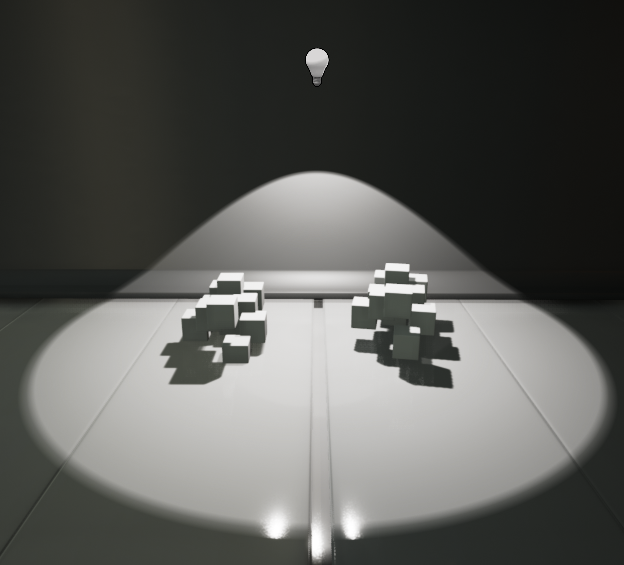
\includegraphics[width=1.\textwidth]{figures/intro/IES_03}
	\end{subfigure}
	\begin{subfigure}[b]{0.293\thewidth}
		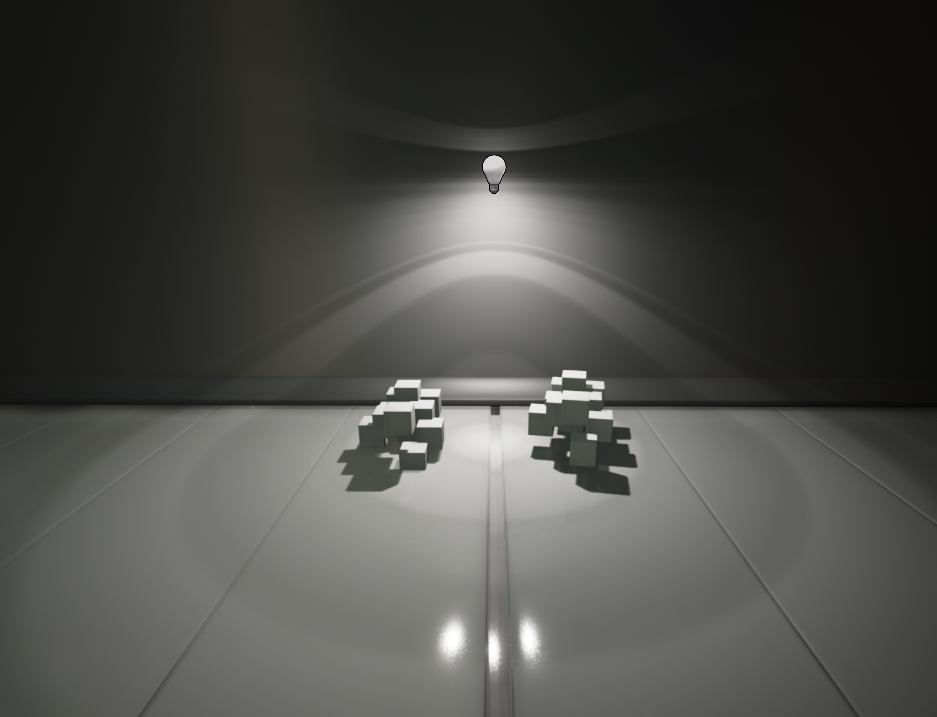
\includegraphics[width=1.\textwidth]{figures/intro/IES_04}
	\end{subfigure}
\caption{在Unreal Engine 4中使用IES光源配置文件定义点光源和聚光灯的光照强度分布 (图片来自\cite{m:IESLightProfiles})}
\label{f:intro-ies}
\end{fullwidth}
\end{figure}

通过第\ref{sec:irradiance}节的内容可知,在计算光与物体表面交互时,表面接收的所有光照使用辐射照度$E$表示,而光源使用辐射强度$I$表示,所以这里就需要使用第\ref{sec:irradiance}节介绍的的平方反比定律,通过$I$来计算$E$,为了方便,这里重新列出该方程如下:

\begin{equation}
	E= \cfrac{I\cos\theta}{r^{2}}
\end{equation}

虽然$E$随着$1/r^{2}$正比增长在物理上是正确的,但是在图形学上通常使用一个不同的函数来描述$E$怎样随着距离的增加而递减。这种函数称为距离递减函数(distance falloff function)\myindex{距离递减函数}{distance falloff function},由此$E$可以表示为:

\begin{equation}
	E=I\cos\theta f_{\rm dist}(r)
\end{equation}

距离递减函数在计算机图形学中被广泛采用,有以下一些原因:首先距离递减函数可以提供更多的控制来达到一些特殊的效果;其次,随着距离的增加,平方反比函数趋近于$0$但却永远不会为$0$,距离递减函数可以通过设定一个最大距离范围,超出这个范围的表面接收的辐射强度为0来大大提高性能;平方反比函数在距离趋近于$0$时趋近于无限大,而距离递减函数可以通过设定一个最大值,避免这种无限大的值出现在着色计算中。

例如以下是Pixar工作室用在电影产品中的距离递减函数\cite{a:LightingControlsforComputerCinematography}:

\begin{equation}
	f_{\rm dist}(d)=\begin{cases}
		M{\rm e}^{s( \cfrac{d}{L})^{\beta}}, & d<L\\
		K( \cfrac{L}{d})^{\alpha}, &d>L
	\end{cases}
\end{equation}

\noindent 这个函数在一个特定的距离$L$处其值为$K$,在距离小于$L$时逐步达到最大值$M$,递减指数$\alpha$用于控制当距离大于$L$时距离递减函数怎样随着距离递减,常数$s$和$\beta$被设定为特定值以保证函数在过渡点处的导数连续:其中$s\equiv {\rm ln}( \cfrac{K}{M})$,而 $\beta\equiv - \cfrac{\alpha}{s}$,如图\ref{f:intro-falloff}所示。

\begin{figure}
\sidecaption
	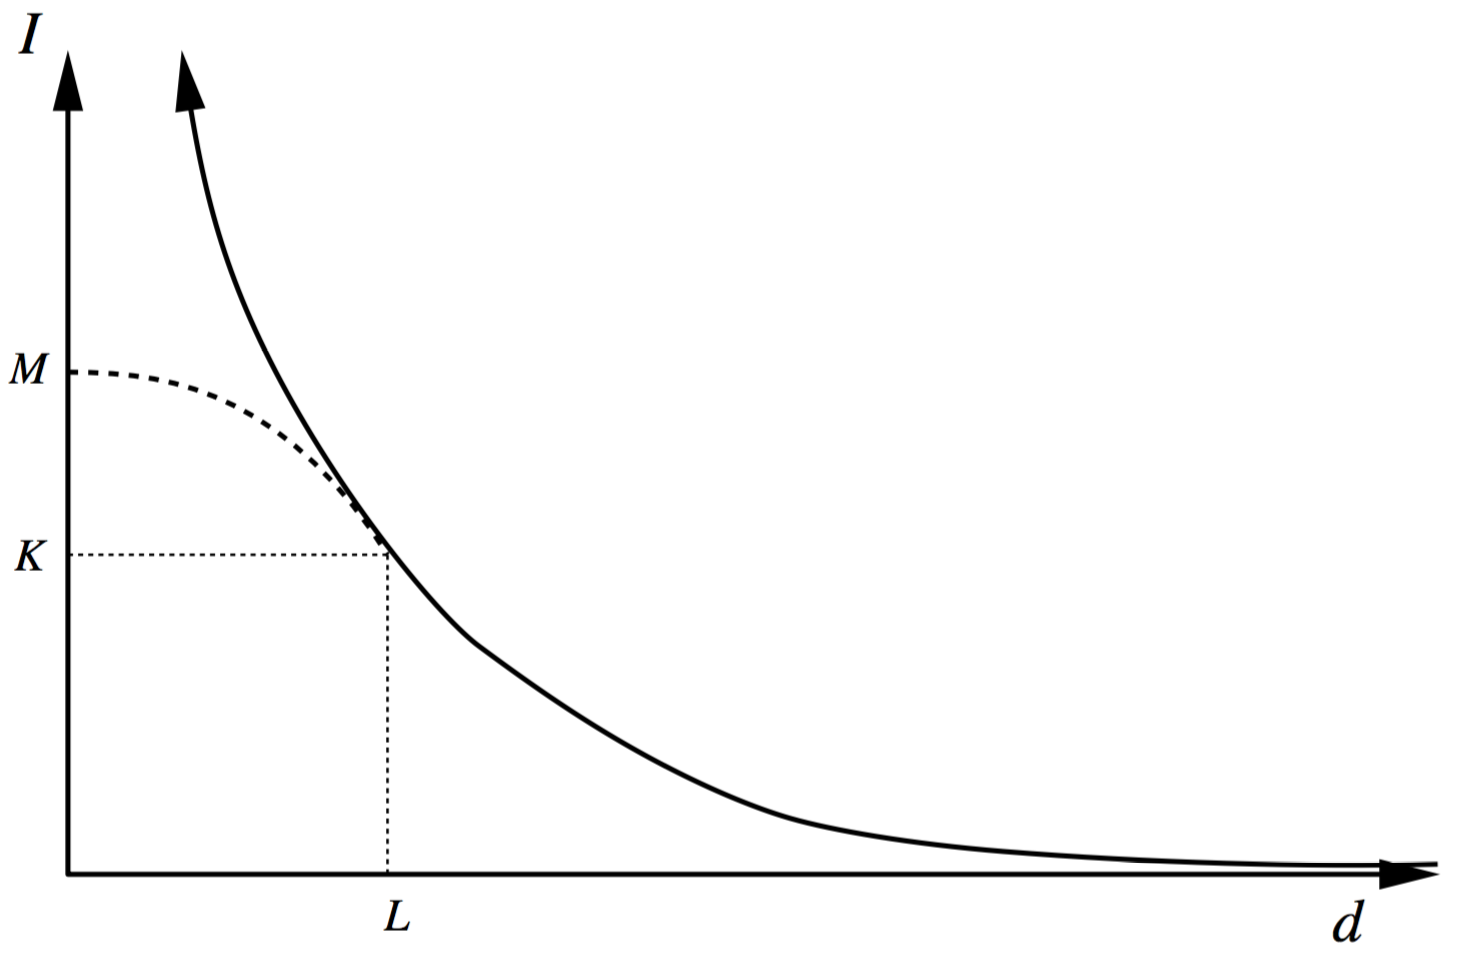
\includegraphics[width=0.6\textwidth]{figures/intro/falloff}
	\caption{Pixar采用的距离递减函数,其中当$d<L$时才有虚线部分,其最大值为$M$}
	\label{f:intro-falloff}
\end{figure}




\subsubsection{材~~质}\label{sec:intro-materials}
光与物体表面交互的一切,都是由材质及其属性来决定的,材质决定了每个物体的表面最终呈现出来的是什么颜色。那么材质到底是什么,这个问题需要从两个方面来理解。

\begin{figure}
\sidecaption
	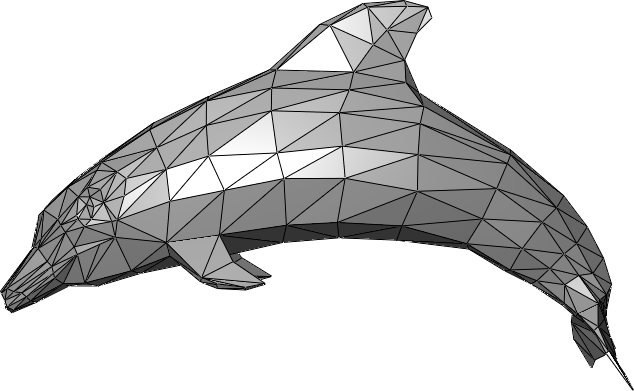
\includegraphics[width=0.4\textwidth]{figures/intro/mesh}
	\caption{一个由三角形网格构成的海豚,网格构成物体的“形”(图片来自Wikipedia)}
	\label{f:intro-mesh}
\end{figure}

首先,在计算机图形学中,一个物体的“形”与“色”是完全分开的,物体的形状由一组顶点(vertex)构成的网格(mesh)来定义,如图\ref{f:intro-mesh}所示,而物体的表面着色则由称为材质(material)\myindex{材质}{material}的东西决定。所以材质通常包含纹理(textures),着色器(shaders)以及其他一些着色方程需要的参数,所有这些数据构成一个对象并被附加到一个物体上,在渲染时这些数据被传输至GPU内存,GPU执行其中的着色器对该物体表面着色,这个过程包括贴图,光照以及其他相关的计算。关于材质的一些重要参数将在下一节讨论。

理解材质的另一方面在于,我们需要了解更多关于物体表面或内部结构的问题。在前面的描述中,都是假设表面是绝对光滑的,在这种情况下,光经过表面时按照反射定律和折射定律进行反射或折射。然而在微观尺度上\footnote{计算机图形学中一般不考虑小于波长的原子尺寸,这又称为纳米几何(nanogeometry)\myindex{纳米几何}{nanogeometry},在此尺寸下可以观察到光的衍射现象,即光可以绕过障碍物沿非直线方向传播。},这里指微观几何(microgeometry)\myindex{微观几何}{microgeometry}结构,即小于一个像素但是大于光波长的尺寸,物体表面并不是绝对光滑的,这时虽然在单个光束与表面交互上可以看作该面是光滑的,但是在一个像素尺度上,它确是不光滑的,如图\ref{f:intro-microgeometry-1}所示。那么我们如何处理这种复杂的情况?

\begin{figure}
\sidecaption
	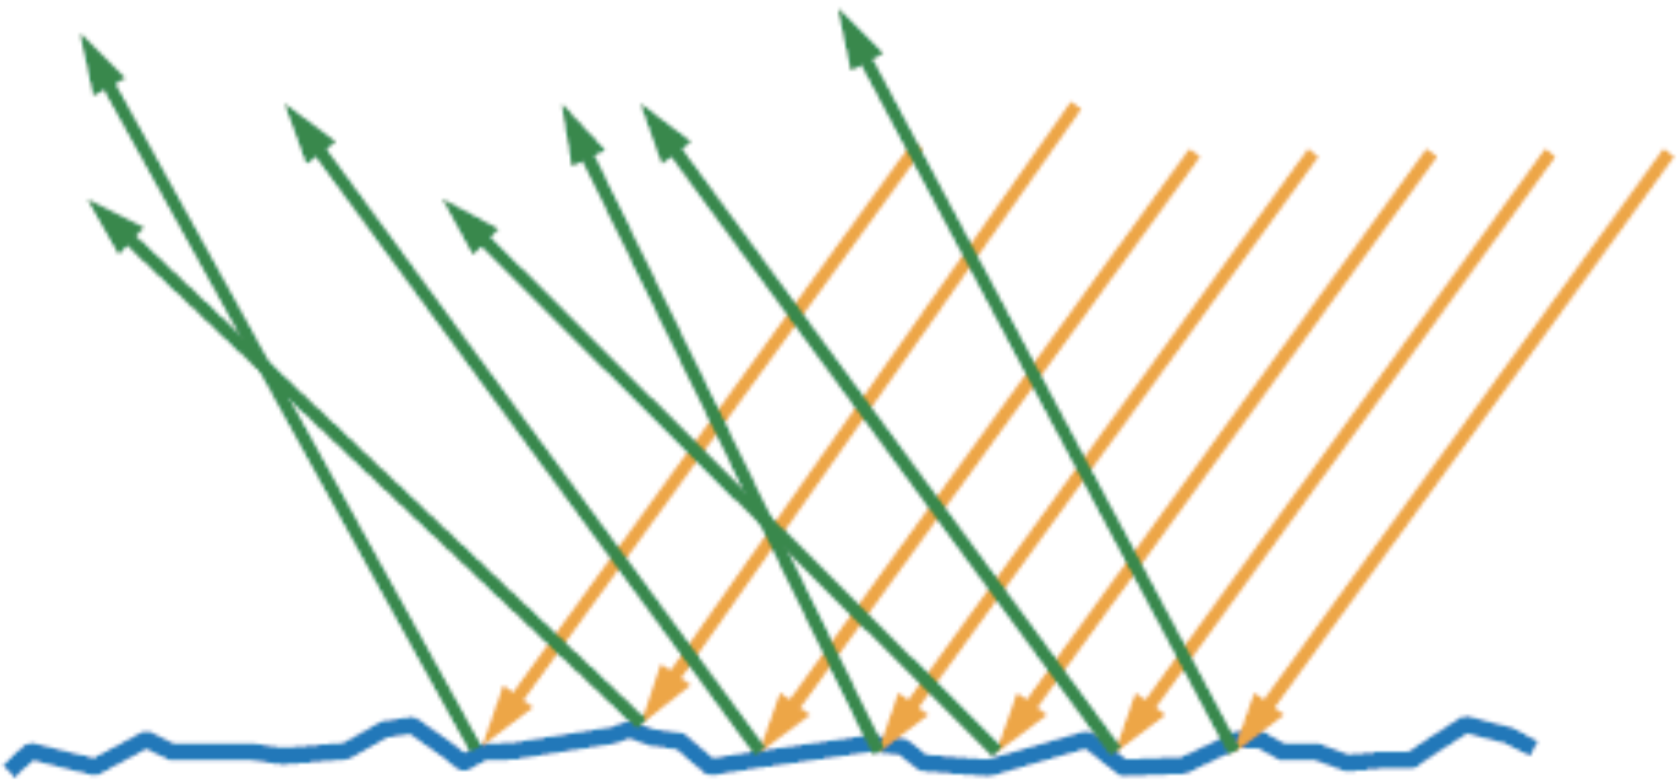
\includegraphics[width=0.4\textwidth]{figures/intro/ray-optics-3}
	\caption{在微观尺寸上,每个点向不同的方向反射或折射光照,注意该图反应的其实是一个像素内的微观尺寸}
	\label{f:intro-microgeometry-1}
\end{figure}

由于表面在微观尺寸上是不光滑的,每个比像素更小的点可能沿不同的方向反射或折射光照,这导致对于一个像素点,每条入射光会被反射或(和)折射至多个方向,如图\ref{f:intro-multi-rays}所示。这等效于是从一个给定的观察方向看,一个像素点可以接受来自多个方向的光照。

\begin{figure}
\sidecaption
	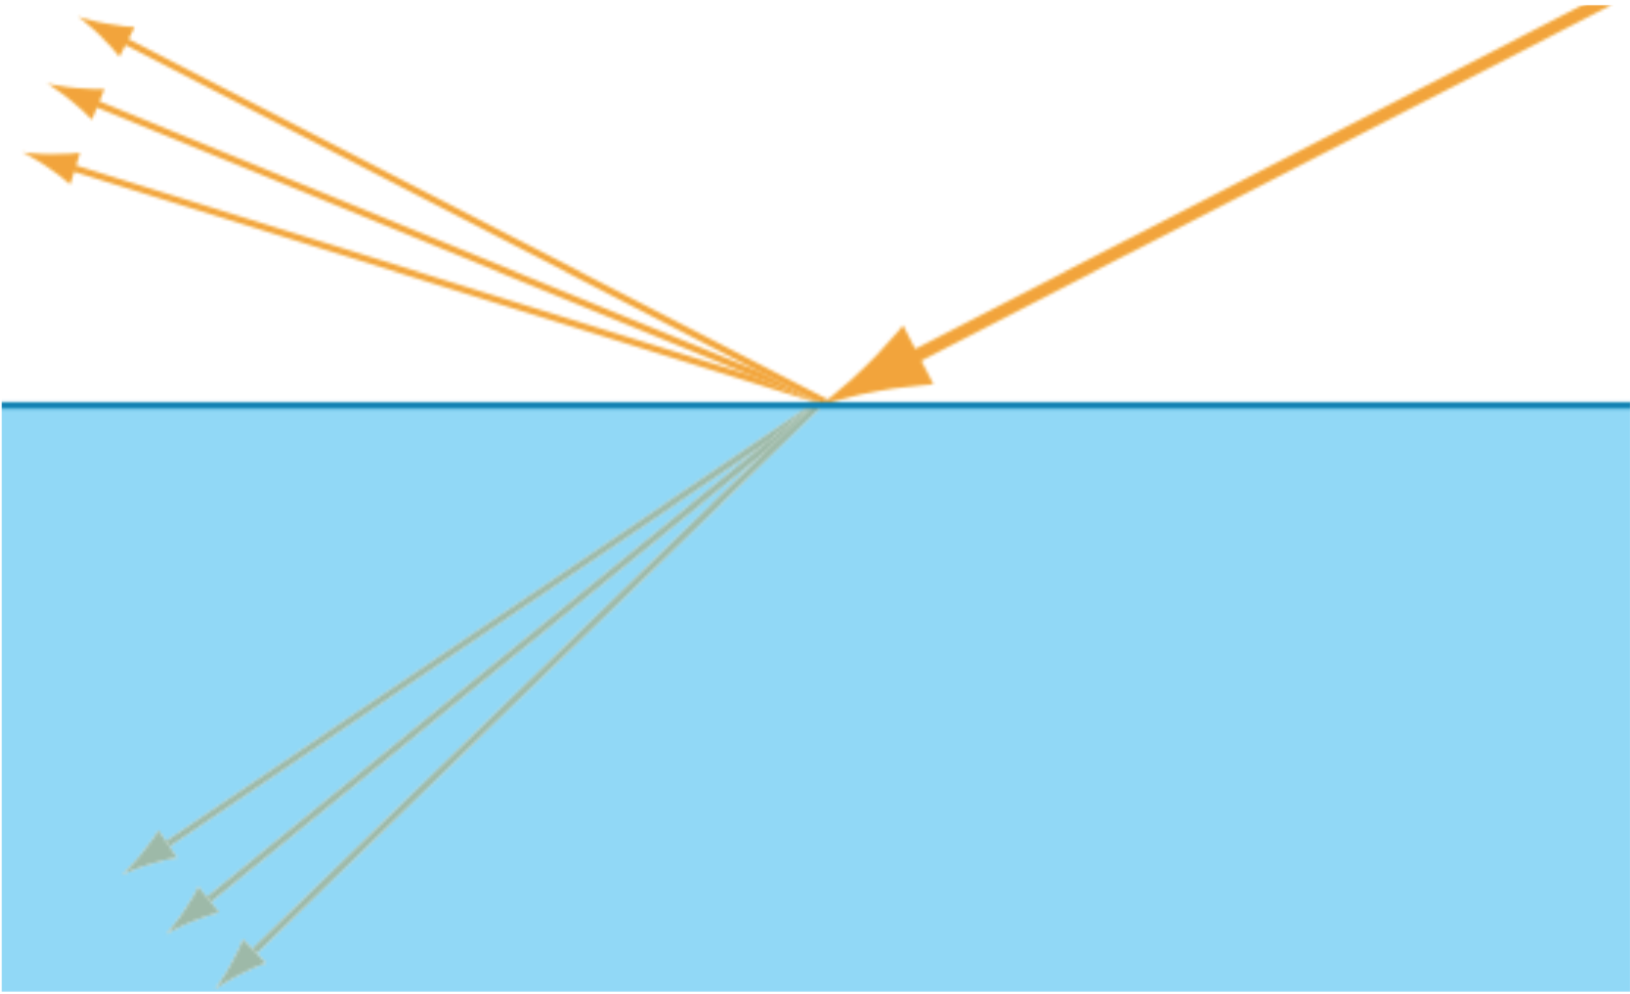
\includegraphics[width=0.5\textwidth]{figures/intro/ray-optics-4}
	\caption{微观结构的粗糙度,导致一个像素点可以将一束像素面积的入射光反射或(和)折射至多个方向}
	\label{f:intro-multi-rays}
\end{figure}

对于折射进物体内部的光照会发生什么呢,这取决于物体材质的结构。在计算机图形学中,材质可以分为两大类\footnote{自然界中还存在第三类材质,即半导体,但是半导体在渲染场景中很少见。}:金属(metals)\myindex{金属}{metals}和非金属,后者又称为绝缘体(insulator)\myindex{绝缘体}{insulator},其中金属立即吸收所有折射的光照。

对于非金属,如果该物体是透明的,如玻璃和水晶,则折射光会在物体内部直线传播,直到遇到该物体另一边的表面后离开物体表面重新回到空气中;对于非透明的物体,由于内部介质的不连续(例如流体,晶体等内部的粒子,泡泡,液滴,瑕疵;有机体表面的粗糙度,细胞;以及衣服布料里的纺织纤维等),折射的光会沿着不同的方向继续反射或者折射,在经历一定的路径之后,这些折射的光部分被重新(可能从原来的位置,也可能从其他位置)发射回到外面,部分可能被吸收。除非该物体是一个完全透明的物体,否则折射的光中总会有部分会发射回到表面外,如图\ref{f:intro-refraction}中的蓝色箭头部分光照,这部分光照可能从不同的位置以不同的方向发射出表面外。值得注意的是,这种由物体内部发射回来的光通常不具有固定的方向性,所以这种反射称为漫散射(scattering)\myindex{漫散射}{scattering}。

\begin{figure}
\sidecaption
	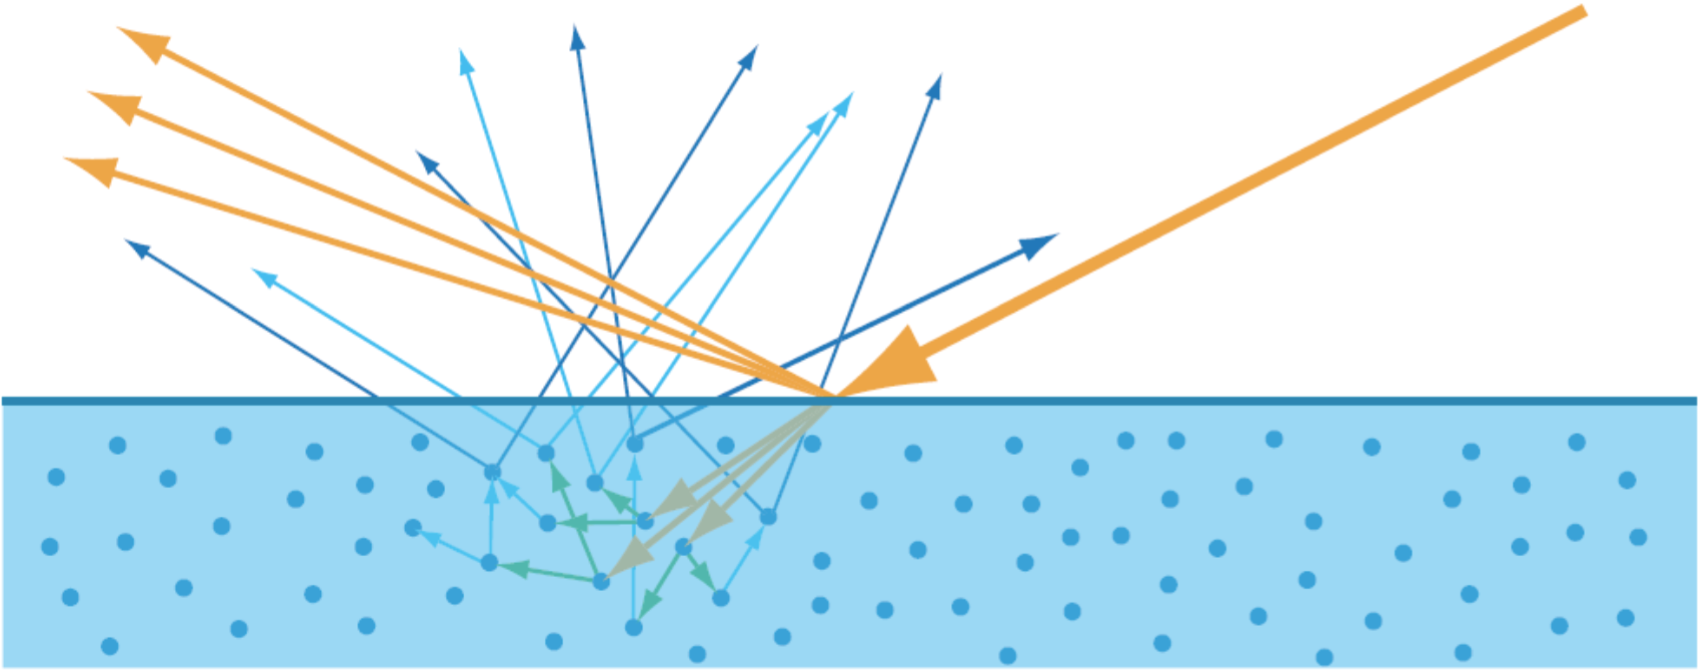
\includegraphics[width=0.65\textwidth]{figures/intro/ray-optics-5}
	\caption{对于非金属材质,经历一定路径的散射之后,部分折射进表面的光会沿不同的方向重新发射回表面外}
	\label{f:intro-refraction} 
\end{figure}

散射光重新发射回表面外的位置与入射点位置之间距离的分布,取决于该物质表面的属性。如果这个距离小于一个像素的尺寸(即在微观范围中),在着色的时候可以假设其距离为$0$,这种散射称为局部次表面散射(local subsurface scattering)\myindex{局部次表面散射}{local Subsurface scattering};否则称为全局次表面散射(global subsurface scattering)\myindex{全局次表面散射}{global subsurface scattering}。在计算机图形学中,这两种现象通常分别使用不同的技术实现。

在计算机图形学中,通常将反射和漫反射这两种不同的光照区分开,分别称为光泽(specular)和漫反射光\footnote{在光学中,漫反射(甚至散射本身)也包含一部分由于物体表面的粗糙度形成的直接反射光的一部分,并不全是由折射进表面的光形成。}(diffuse)。其中前者主要由于光在物体表面的直接反射形成,而后者通常由光进入物体表面,经历折射,吸收,多次散射过程之后重新从物体表面散射回表面外的光形成,如图\ref{f:intro-specular-and-diffuse}所示。这样区分的目的也在于由于漫反射光可以接收来自全部方向的光,因此需要对全空间进行积分计算,但是将与方向无关的部分分离出来,则可以使用更简单的方法处理漫反射,关于这些方法将在本章及本书后面介绍。

\begin{figure}
\sidecaption
	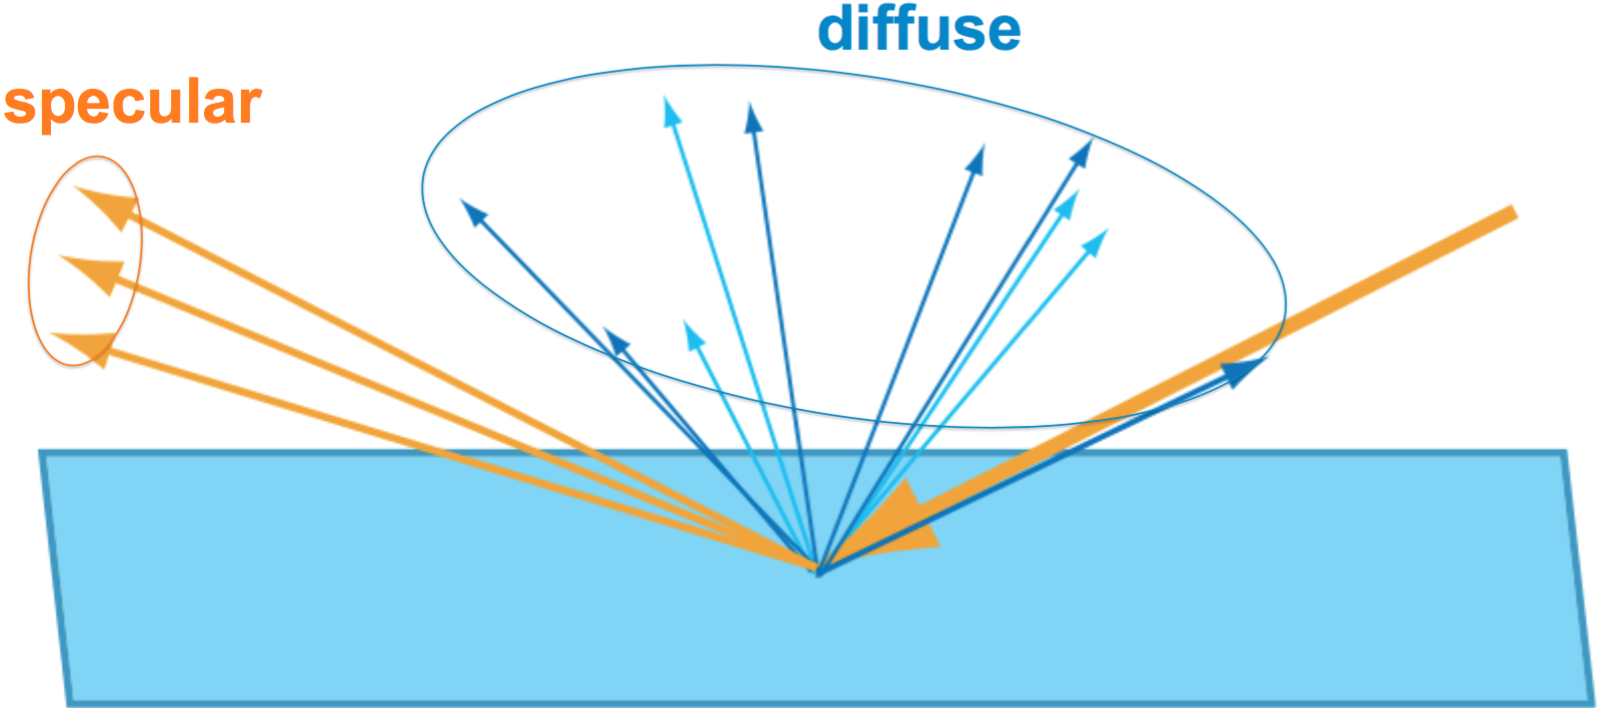
\includegraphics[width=0.6\textwidth]{figures/intro/ray-optics-6}
	\caption{光与物体表面交互后反射的光可以分为光泽和漫反射光两部分}
	\label{f:intro-specular-and-diffuse}
\end{figure}

对于光泽部分,这些反射光所处范围的大小取决于表面的粗糙度(下一节会讨论),表面越粗糙,则反射的范围越大,物体表面越模糊;反之表面越光滑,反射的范围越小,则表面越光亮,如图\ref{f:intro-roughness}所示。

\begin{figure}
\sidecaption
	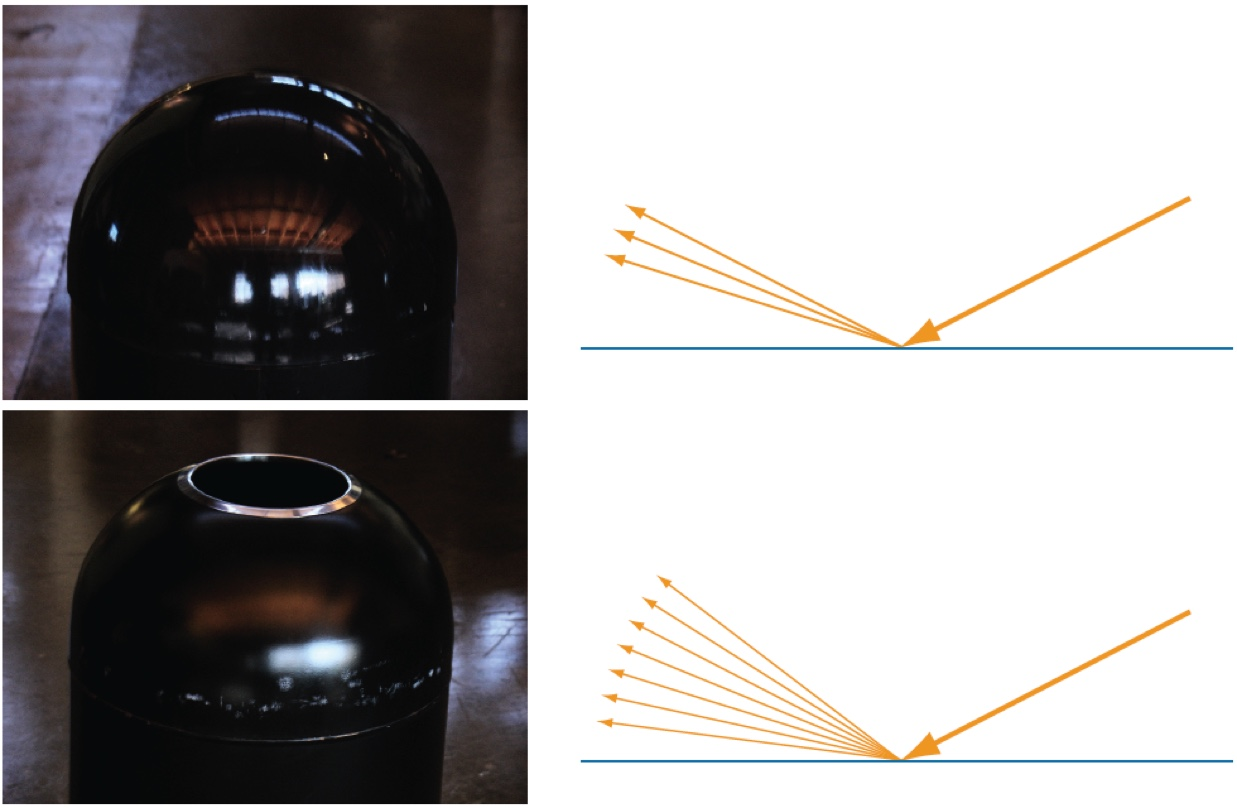
\includegraphics[width=0.65\textwidth]{figures/intro/ray-optics-2}
	\caption{反射光的范围大小取决于物体表面的粗糙度,物体表面越粗糙,它越能接收更大范围的光照}
	\label{f:intro-roughness}
\end{figure}

由于材质决定物体表面的着色,所以上述所有这些现象都需要在材质中进行表述,对于如漫反射率等这种与观察方向无关的参数,它们可以通过纹理的方式存储并关联到材质中;而对于与方向有关的这些反射特征,它们可能以函数的形式存在于着色器代码中,例如上述关于表面的光泽反射特征可以通过本章后面介绍的微面元理论来进行表述。





\subsubsection{感应器}\label{sec:intro-sensor}
当光从光源发射出,并在场景中与物体表面进行多次交互后,最终其中的一部分会进入图像传感器形成图像。由于图像传感器接收的是辐射亮度$L$(其值由渲染管线中的像素着色器计算出),并且数字图像以一定的分辨率存储图像信息,所以可以使用图\ref{f:intro-camera}来表示计算机图形学中的图形传感器成像系统,这里$P$点就是场景中的“摄像机”对象,摄像机朝着虚拟屏幕中的每个像素的方向发射一条射线,称为观察矢量(view vector)\myindex{观察矢量}{view vector} $\mathbf{v}$(它也是着色器计算中渲染方程的出射方向),场景中所有沿$\mathbf{v}$反方向传播的光线就会进入摄像机。

\begin{figure}
\sidecaption
	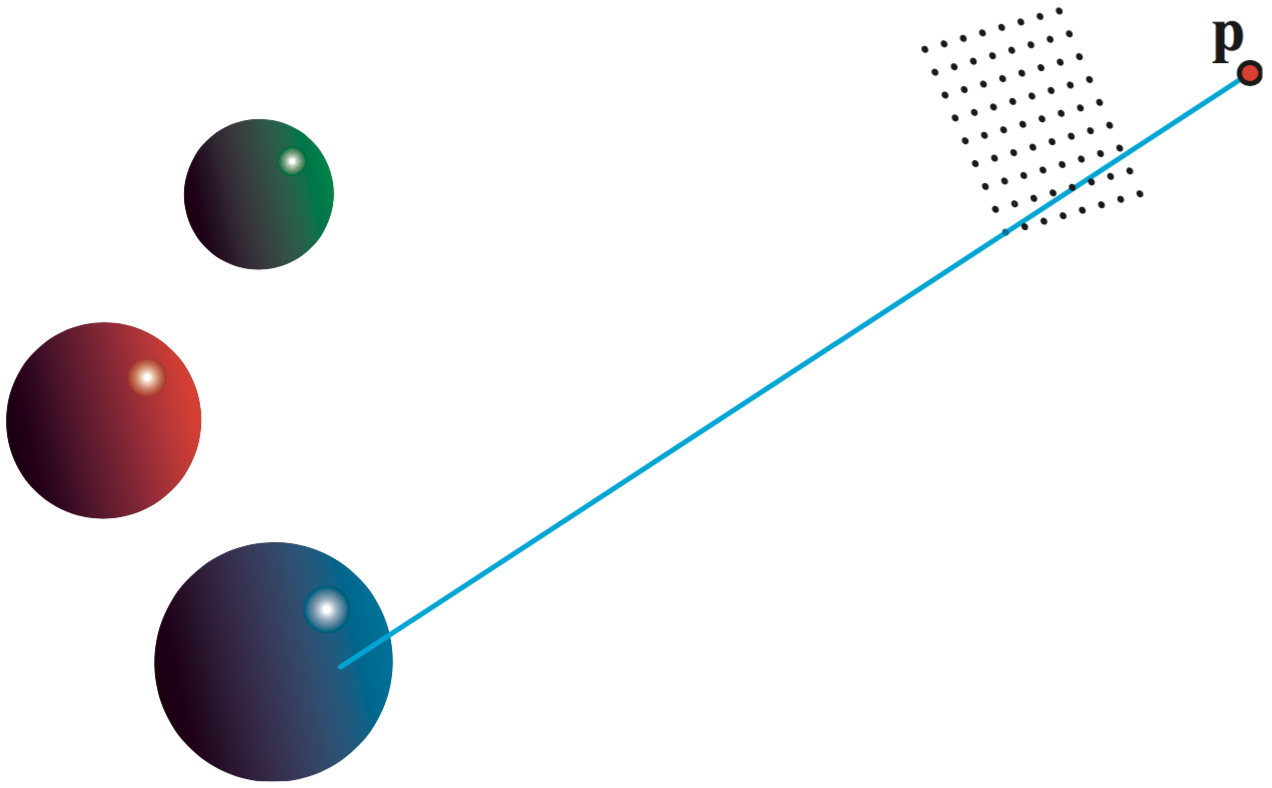
\includegraphics[width=0.6\textwidth]{figures/intro/camera}
	\caption{理想的计算机图形学图像传感器模型,其中${\rm p}$为摄像机或观察点,中间的点阵为屏幕的像素网格,左边的球体为场景中的物体}
	\label{f:intro-camera}
\end{figure}

然而事情并不像这么简单,对于给定分辨率的“屏幕”,它的每一个像素点总是有一个尺寸大小的。而对于每个像素,我们通常取其从摄像机发出穿过该像素中心点的方向对场景进行采样,如果一个像素的中心点被三角形覆盖,则整个像素区域被填充一个单一的颜色,否则即使该像素有小部分区域被覆盖,它也不会被填充任何颜色,这使得三角形的边缘出现锯齿(jaggies)\myindex{锯齿}{jaggies},如图\ref{f:intro-aliasing-triangle}所示。这种锯齿是由于采样不足导致的一种走样(aliasing)\myindex{走样}{aliasing}现象,而尝试避免或者减少这种走样的技术称为反走样(anti-aliasing)\myindex{反走样}{anti-aliasing}技术。

\begin{figure}
\sidecaption
	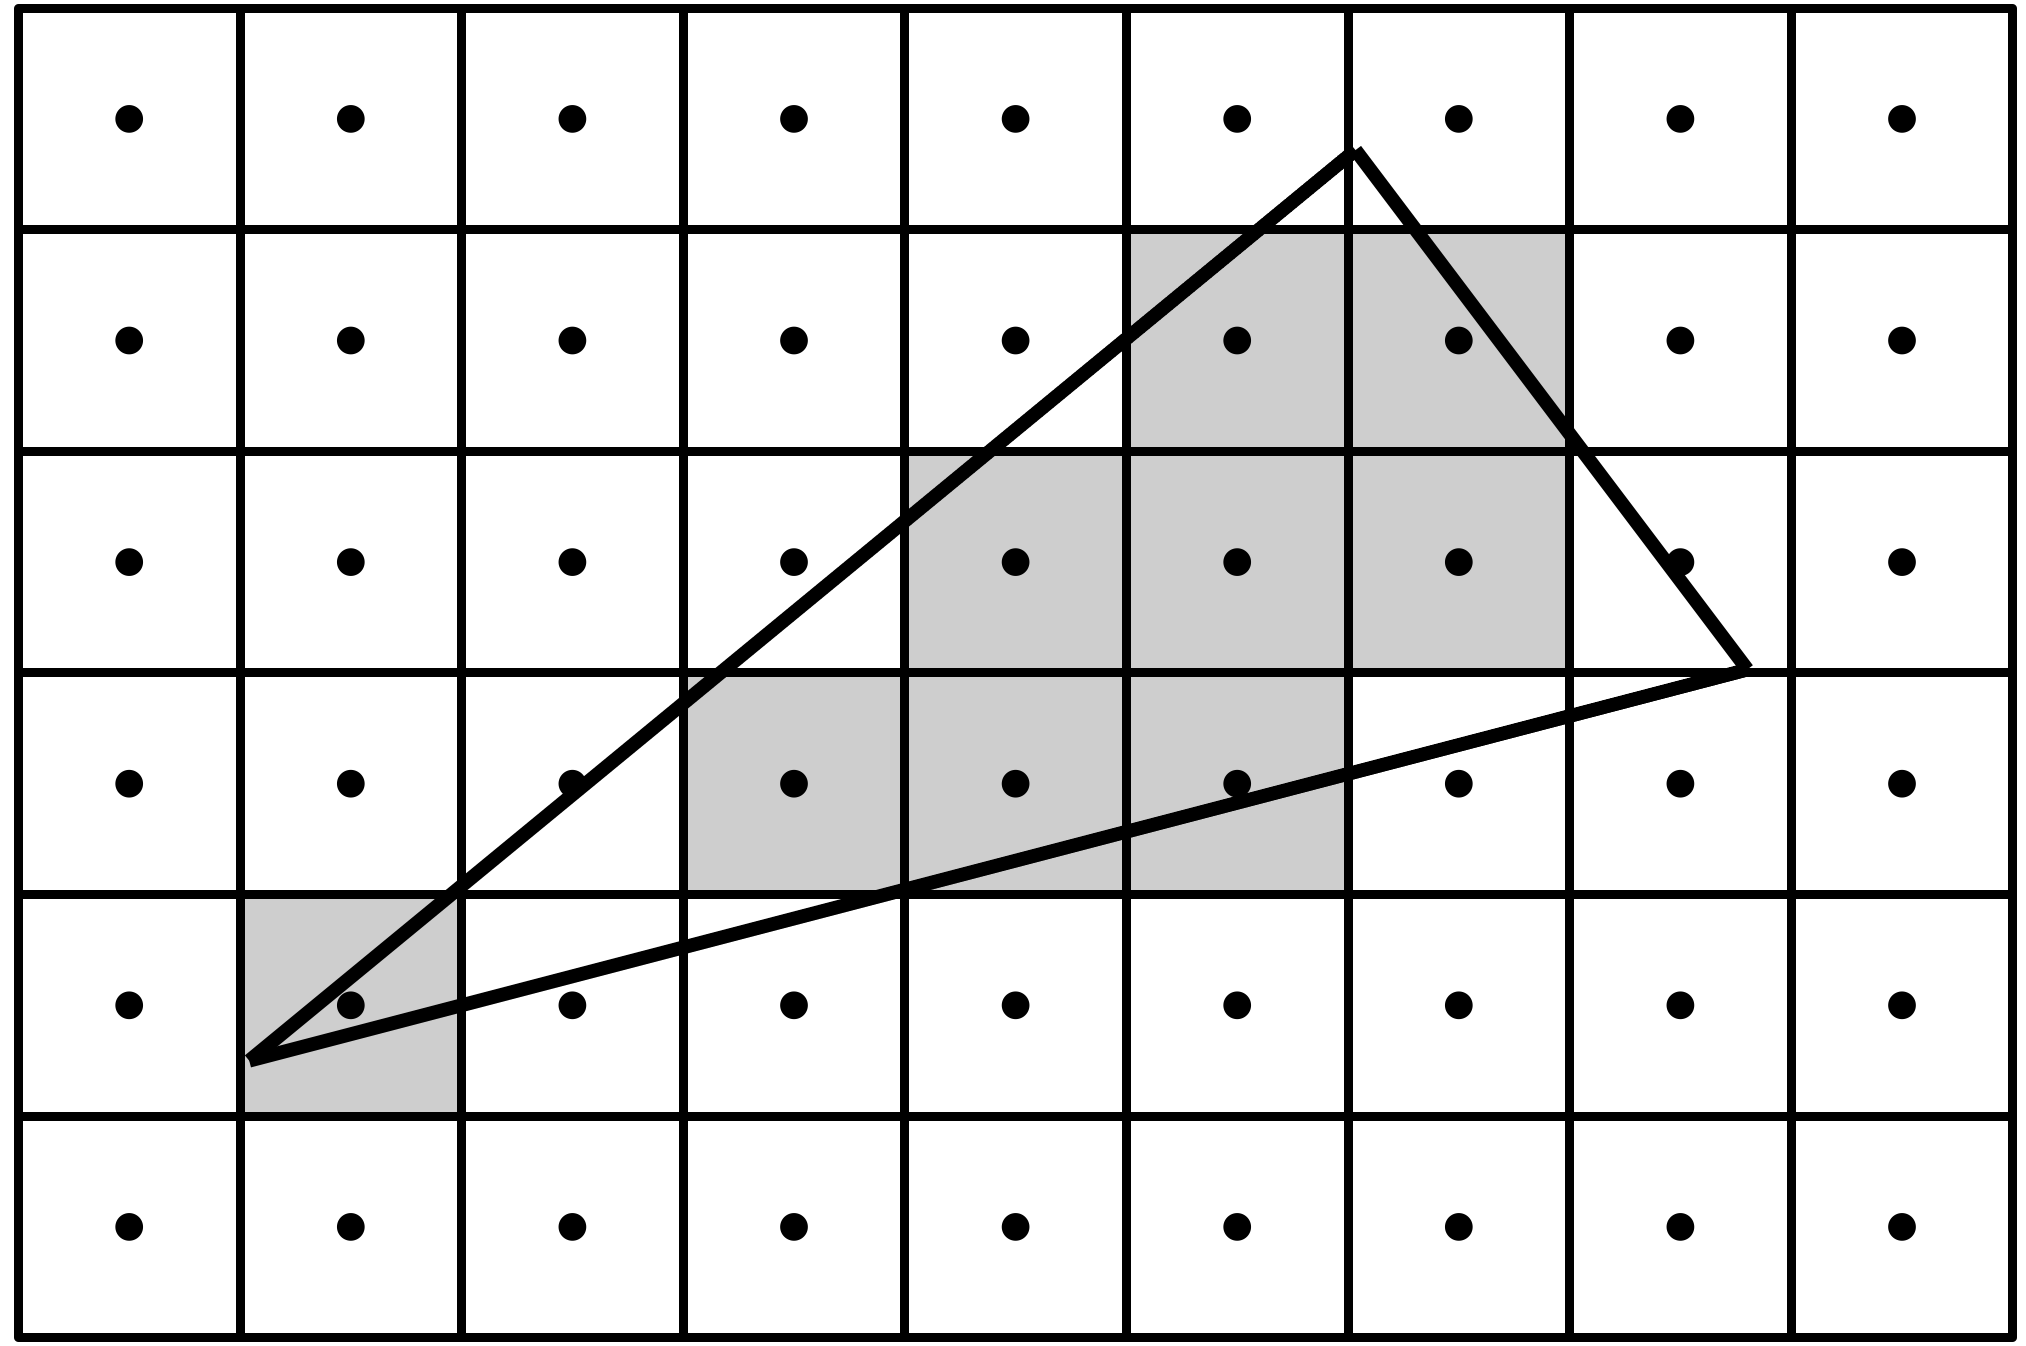
\includegraphics[width=0.45\textwidth]{figures/intro/aliasing-triangle}
	\caption{光栅化技术通过测试几何图形对像素中心点的覆盖来决定是否对该像素点着色,这造成在几何图形的边缘出现锯齿的现象}
	\label{f:intro-aliasing-triangle}
\end{figure}

用数学理论来解释和解决这种缺陷,涉及数字信号处理的一些理论,如采样,重建,走样等。这些技术的学习不仅有助于理解渲染过程中数字图像的生成过程,它也是计算机图形学的重点内容,例如着色器中对纹理的采样,后处理中很多都涉及走样技术等等。接下来,我们将讨论关于数字信号处理的一些理论,并解释这些理论怎样被用在计算机图形学中。

	



\section{采样和反走样}\label{sec:intro-sampling}
3D图像的生成本质上是一个对各种连续函数(如几何图形,BRDF分布函数,光照场等)采样,然后转化为对应的一个离散函数(以有限分辨率表示的一个二维图像)的过程。3D渲染的大部分采样发生在光栅化阶段,或者其他由光栅化导致的采样,例如图\ref{f:intro-aliasing-triangle}中,三角形两个顶点之间的边是连续的,但是被光栅化过程采样为离散的像素值。

在数字信号处理(digital signal processing)\myindex{数字信号处理}{digital signal processing}中,术语采样(sampling)\myindex{采样}{sampling}的目的是将连续的信号表述为离散的信号,在采样的过程中,其中的一些信息会丢失;为了重建(reconstruction)\myindex{重建}{reconstruction}原始连续信号,则需要对离散信号使用过滤(filtering)\myindex{过滤}{filtering}技术来还原原始连续信号,如图\ref{f:intro-signal-processing}所示。

\begin{figure}
\begin{fullwidth}
	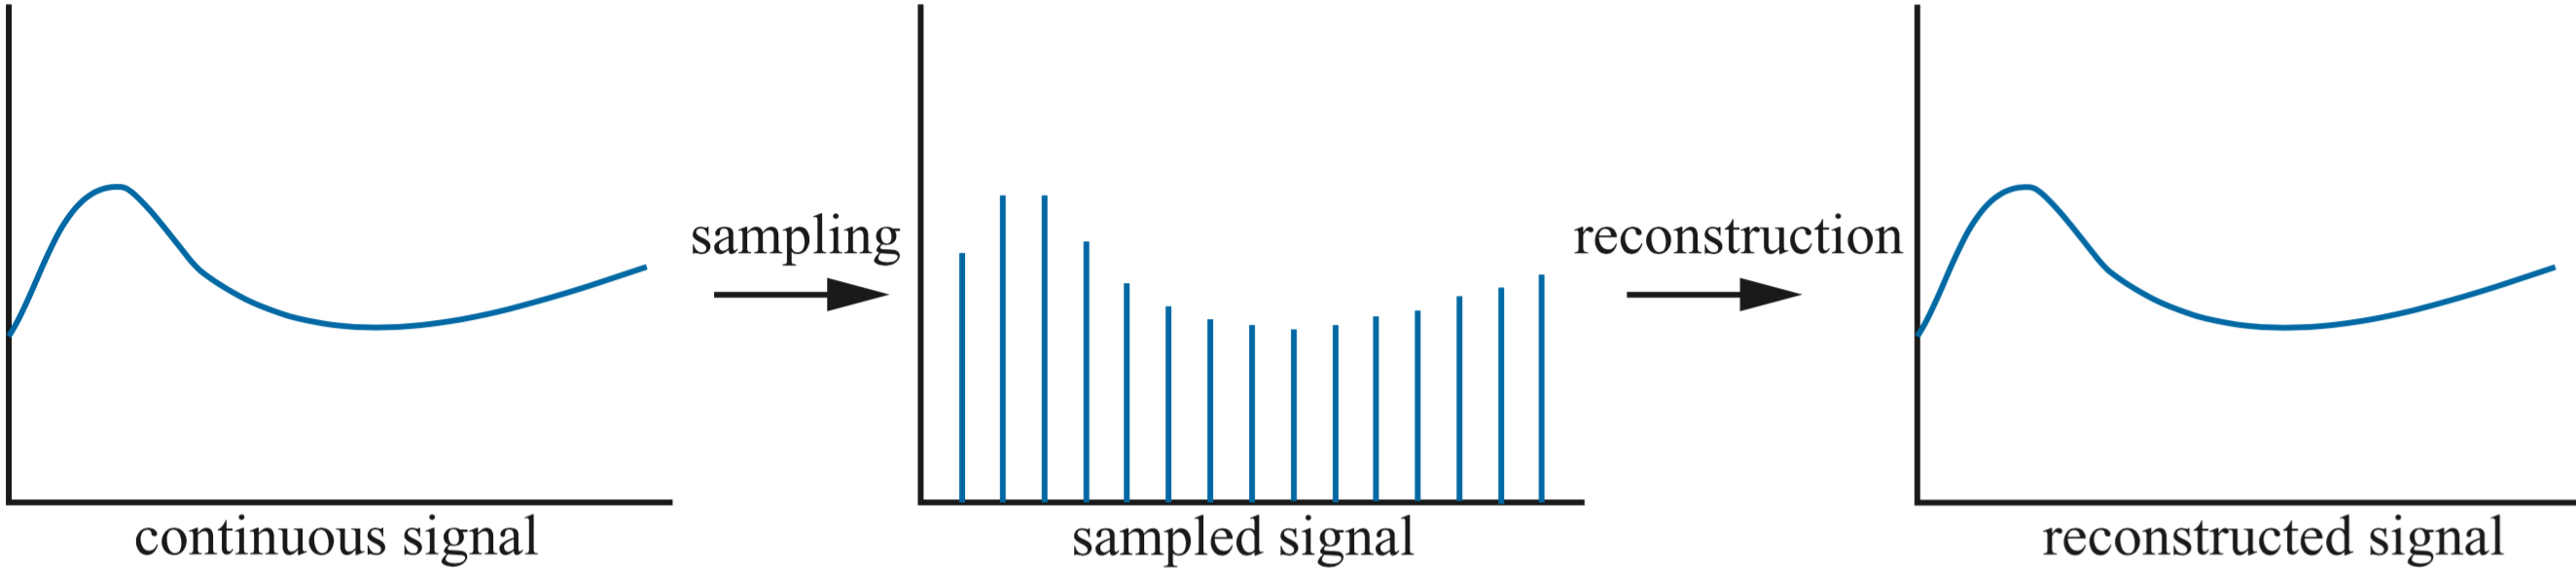
\includegraphics[width=1.\thewidth]{figures/intro/signal-processing}
	\caption{在数字信号处理的过程中,一个连续的信号(左图)被采样为离散的信号(中图),然后通过重建还原为接近原连续信号的连续信号(右图)}
\label{f:intro-signal-processing}
\end{fullwidth}
\end{figure}

以下我们就首先来讨论采样和重建这两个数字信号处理的基本过程,然后介绍一些由于采样不足导致的走样的概念以及其一般解决方案。




\subsection{采~~样}\label{sec:intro-sampling}\myindex{采样}{sampling}
关于采样的理论非常复杂,它涉及傅里叶变换,积分,级数等数学知识,以及像频率域等滤波相关的概念。然而理解采样相关知识是理解走样相关知识的重要理论基础,而且在图形学的其他一些地方也会涉及这些知识,例如在光线追踪技术中就会大量涉及脉冲函数。此外,理解傅里叶变换也有助于理解后面的如小波变换,球谐函数等概念。但本节不会严格地推导和讨论傅里叶相关的知识,而只是使用一些结论让读者比较容易地理解采样相关的概念及逻辑,本书后面的内容还会反复更深入地讨论傅里叶变换相关的知识,更多关于数字图像处理的理论知识,可以参考\cite{b:DigitalImageProcessing}。

法国数学家傅里叶(Jean Baptiste Joseph Fourier)于1807年在他的《热分析理论》一书中指出,任何非周期\footnote{对于任何周期函数则可以使用傅里叶级数,表示为不同频率的正弦和/或余弦和的形式,每个正弦项和/或余弦项乘以不同的系数。例如具有周期$T$的周期函数$f(t)$的傅里叶级数为:

\begin{equation}\label{eq:fourier-series}
	f(t)=\sum^{\infty}_{n=-\infty}c_n {\rm e}^{j \cfrac{2\pi n}{T}t}
\end{equation}

\noindent 其中:

\begin{equation}
	c_n= \cfrac{1}{T}{\rm \int}^{T/2}_{-T/2}f(t){\rm e}^{-j \cfrac{2\pi n}{T}t}{\rm d}t, n=0,n=\pm 1,n=\pm 2,\cdots
\end{equation}

}(但该曲线下的面积是有限的)的连续函数可以用正弦和/或余弦乘以一个加权函数的积分来表示,这个积分方程称为傅里叶变换(Fourier transform)\mathindex{傅里叶变换}{Fourier transform}。用$F(\mu)$表示连续变量$t$的连续函数$f(t)$的傅里叶变换,则:

\begin{equation}\label{eq:intro-fourier}
	F(\mu)={\rm \int}^{\infty}_{-\infty}f(t){\rm e}^{-j2\pi\mu t}{\rm d}t
\end{equation}

\noindent 其中,$\mu$表示正弦项或余弦项的频率,由于被积函数中的变量$t$被积分,所以上式的结果为变量$\mu$的函数。

相反,给定$F(\mu)$,通过傅里叶反变换可以获得$f(t)$:

\begin{equation}
	f(t)={\rm \int}^{\infty}_{-\infty}F(\mu){\rm e}^{-j2\pi\mu t}{\rm d}\mu
\end{equation}

\noindent 利用欧拉公式\footnote{${\rm e}^{j\theta}=\cos\theta +j\sin\theta$},可以把式\ref{eq:intro-fourier}表示为:

\begin{equation}
	F(\mu)={\rm \int}^{\infty}_{-\infty}f(t)[\cos (2\pi\mu t)-j\sin(2\pi\mu t)]{\rm d}t
\end{equation}

我们看到,由于变量$t$被积分后只剩下$\mu$,所以傅里叶变换$F(\mu)$的作用域是频率域。频率变量$\mu$的单位取决于$t$的单位,例如,如果$t$表示单位为秒的时间,则$\mu$的单位为周/秒,如果$t$表示单位为米的时间,则$\mu$的单位为周/米。

从广义上讲,频率域(frequency domain)\myindex{频率域}{frequency domain}表述的是一个连续函数在它的作用域上的改变有多快,所以一个函数通常有多个频率,这些频率构成该函数的一个频率谱(spectrum of frequencies)\myindex{频率谱}{spectrum of frequencies}。傅里叶变换正是将一个连续非周期函数由其时间域\footnote{如果一个信号随时间而变化,称该作用域为时间域。}(time domain)\myindex{时间域}{time domain}或空间域\footnote{例如与时间无关的静止的图像,它的作用域为空间位置$x,y,z$,称为空间域。}(spatial domain)\myindex{空间域}{spatial domain}变换到其频率域。其目的在频率域我们可以发现该函数的一些重要特征,甚至一些对函数的操作在频率域进行更方便。

从图\ref{f:intro-fourier}中可以看到这种作用域的转化,红色线条代表原始连续周期函数(注意这里是针对傅里叶级数而非傅里叶变换进行描述),蓝色线条为傅里叶级数各级的正弦或余弦函数,图\ref{f:intro-fourier}(a)包含了傅里叶级数的头6项,这个傅里叶级数本身是有无穷多项的。图\ref{f:intro-fourier}(b)通过提取出每个正弦或余弦项的频率,而形成图\ref{f:intro-fourier}(c)的频率域函数,这个频率域将用于后面对信号采样的质量判定。值得注意的是,由式\ref{eq:fourier-series}可知,其傅里叶级数的频率域是离散的;然而由式\ref{eq:intro-fourier}可知,非周期连续函数的频率域函数,即傅里叶变换函数是连续的,如图\ref{f:intro-fourier-case}所示。

\begin{figure}
\begin{fullwidth}
	\begin{subfigure}[b]{0.33\thewidth}
		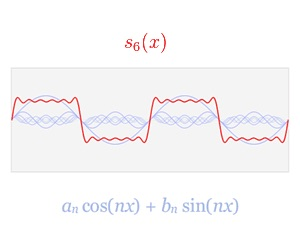
\includegraphics[width=1.\textwidth]{figures/intro/fourier-1}
		\caption{傅里叶级数头6项}
	\end{subfigure}
	\begin{subfigure}[b]{0.33\thewidth}
		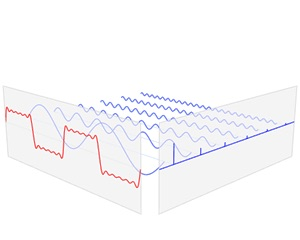
\includegraphics[width=1.\textwidth]{figures/intro/fourier-2}
		\caption{傅里叶变换}
	\end{subfigure}
	\begin{subfigure}[b]{0.33\thewidth}
		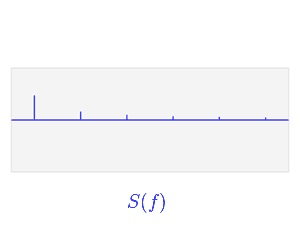
\includegraphics[width=1.\textwidth]{figures/intro/fourier-3}
		\caption{频率域}
	\end{subfigure}
\caption{傅里叶变换将函数由时间域(或空间域)变换到频率域,注意这里讨论的是周期函数的傅里叶级数(图片来自Wikipedia)}
\label{f:intro-fourier}
\end{fullwidth}
\end{figure}

当一个函数被变换到频率域后,则我们可以检测该函数是否存在最大的频率,以至对于所有大于该频率的傅里叶变换函数的值为$0$。如果该最大频率存在,该函数称为带限函数(bandlimited function)\myindex{带限函数}{bandlimited function},这意味着我们可以检测该函数的频率带宽(bandwidth)\myindex{频率带宽}{bandwidth},如图\ref{f:intro-fourier-case}是某个函数的傅里叶变换,其频率带宽为$2B$。带限函数是后面对函数进行采样以及相关理论的重要基础概念。

\begin{figure}
\sidecaption
	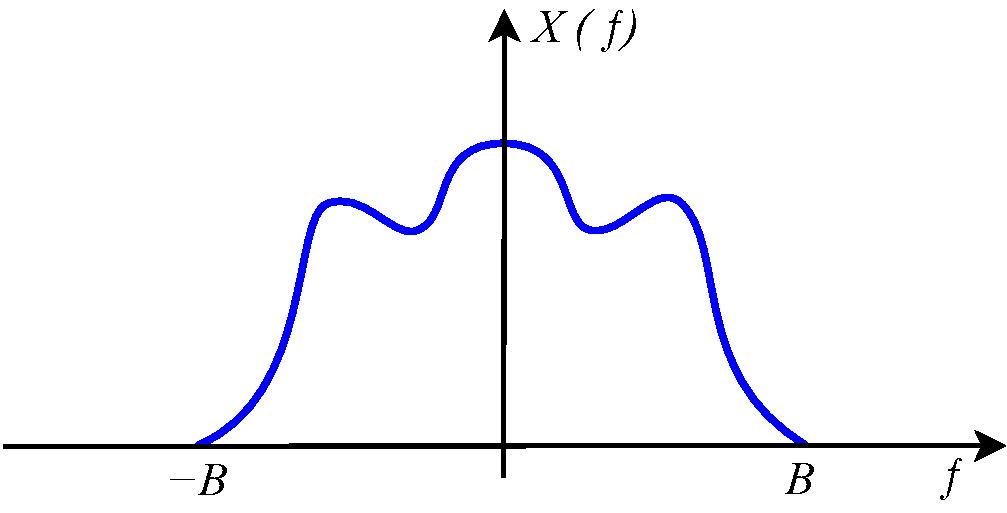
\includegraphics[width=0.6\textwidth]{figures/intro/Bandlimited}
	\caption{一个带限函数的频率域具有一个有限的范围,如果采用频率大于这个带限的宽度,则其采样后的离散信号可以被完美复原(图片来自Wikipedia)}
	\label{f:intro-fourier-case}
\end{figure}

为了理解采样及采样定理,我们需要首先了解一下卷积的概念,卷积在计算机图形学中也是一个重要的基础数学工具,例如在后面讨论渲染方程,以及一些全局光照方案中几乎所有涉及球谐函数(spherical harmonics)\myindex{球谐函数}{spherical harmonics}的地方等都会涉及卷积,所以本节首先学习卷积及其在傅立叶变换中的应用。




\subsubsection{卷~~积}
在数学上,卷积(用符号$\star$表示)定义为两个函数$f$和$g$,在其中一个函数被翻转$180^{\circ}$之后(以下假设$g$被翻转),两个函数乘积的积分,即:

\begin{equation}\label{eq:intro-conv}
	f(t)\star g(t)={\rm \int}^{\infty}_{-\infty}f(\tau)g(t-\tau){\rm d}\tau
\end{equation}

\noindent 注意这里$\tau$是一个积分假变量,它说明在积分滑过整个定义域的同时,翻转函数$g$将作用于$f$的每一个位置。

我们可以给卷积做一个很直观的视觉解释,在图\ref{f:intro-Convolution}中,蓝色曲线表示函数$f$,红色曲线表示函数$g$,以下过程可以用来描述卷积的计算:

\begin{figure}
	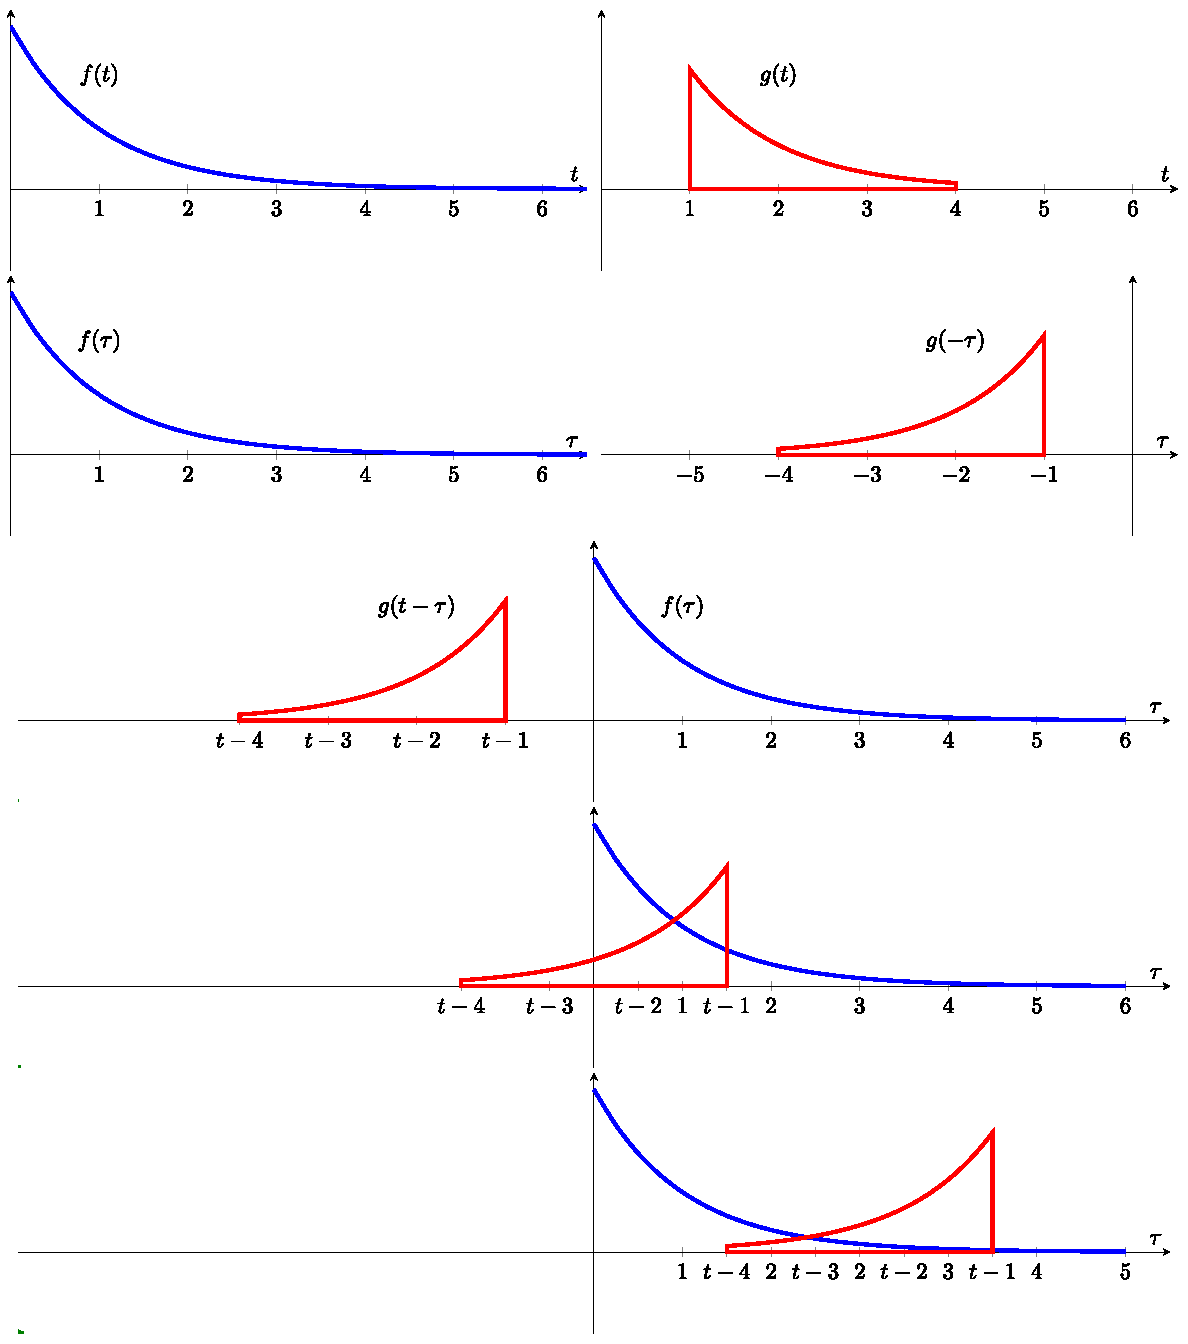
\includegraphics[width=\textwidth]{figures/intro/Convolution}
	\caption{卷积的视觉解释,对于两个函数$f$和$g$的卷积(第一行),我们首先将$g$执行$180^{\circ}$翻转(第二行),然后将$g(t-\tau)$从定义域的左边(第三行)开始向右滑动(第四,五行),并在每个位置$t$处计算式\ref{eq:intro-conv}中的积分(图片来自Wikipedia)}
	\label{f:intro-Convolution}
\end{figure}

\begin{enumerate}
	\item 对函数$g$执行$180^{o}$翻转: $g(\tau )\to g(-\tau )$,如图\ref{f:intro-Convolution}第一行到第二行的图形变化。
	\item 设置一个时间偏移$t$,使$g(t-\tau )$从$\tau-$轴的起点位置开始“滑行”,如图\ref{f:intro-Convolution}第三行所示。
	\item 将$t$从$-\infty$滑动到$\infty$,即是将$g$从$-\infty$沿$\tau-$轴滑动到$\infty$经过整个时间域,如图\ref{f:intro-Convolution}第四和五行所示,只要两个函数存在相交,则计算它们乘积的积分,换句话说,在每个时间$t$,对$f(\tau )$执行一个权重系数为$g(-\tau )$的积分,注意式\ref{eq:intro-conv}的积分变量为$\tau$,它表示被执行翻转的函数$g$的作用域,所以整个积分是一个关于$t$的函数,我们需要求解每个$t$处的积分。
\end{enumerate}

这个过程形成的关于$t$的波形(在图中没有画出),即是$f$和$g$的卷积。由此可以看出,卷积计算是对$f$整个定义域的每一点,在$g$定义域内的积分计算。因此卷积的计算量非常大,我们看到后面的一些计算中,$g$的定义域一般都非常小。此外,卷积是一个线性计算,它输出一个和$f$定义域一样大小的结果,例如,如果$f$代表的是一张图像,则卷积计算的结果输出另一张一样大小的图像。另外,卷积公式本身只是关于每个点$t$的计算公式,所以卷积实现必须要遍历整个$f$定义域。

对于卷积和傅里叶变换,可证明(读者可参考\cite{b:DigitalImageProcessing}等相关书籍),空间域中两个函数的卷积的傅里叶变换等于两个函数的傅里叶变换在频率域的乘积;反过来,如果有两个变换的乘积,则可以通过计算傅里叶反变换得到空间域的卷积,这即是卷积定理(convolution theorem)\mathindex{卷积定理}{convolution theorem}。换句话说,$f(t)\star h(t)$和$H(\mu)F(\mu)$是傅里叶变换对,这一结果是卷积定理的一半,可以写为:

\begin{equation}
	f(t)\star h(t)\Leftrightarrow H(\mu)F(\mu)
\end{equation}

双箭头用于指示右边的表达式是通过对左边的表达式执行傅里叶变换得到的,而左边的表达式是通过求右边表达式的傅里叶反变换得到的。

遵循类似的推导可得到卷积定理的另一半:

\begin{equation}
	f(t)h(t)\Leftrightarrow H(\mu)\star F(\mu)
\end{equation}

\noindent 它说明频率域的卷积类似于空间域的乘积,两者分别与傅里叶正,反变换相联系。卷积定理是傅里叶分析的重要基础,也是计算机图形学中很多算法的重要基础工具。



\subsubsection{采样定理}
有了傅里叶变换和卷积定理两个基础工具,我们就可以推导出采样定理,由于信号处理涉及对连续信号进行采样,以生成离散信号,然后通过离散的采样结果对函数进行重建的过程,采样定理告诉我们,在什么条件下可以完美地重建原始连续信号。除此之外,采样定理还能帮助我们理解走样的概念,以及对离散信息进行平滑等知识。

首先我们需要了解冲激函数(dirac function)\mathindex{冲激函数}{dirac function}的概念,它是推导采样定理的重要基础。连续变量$t$在$t=0$处的单位冲激表示为$\delta(t)$,其定义为:

\begin{equation}
	\delta(t)=\begin{cases}
		\infty & t=0\\
		0      & t\neq 0
	\end{cases}
\end{equation}

\noindent 同时它还被限制为满足:

\begin{equation}
	\int^{\infty}_{-\infty}\delta(t){\rm d}t=1
\end{equation}

很容易看出,假设函数$f(t)$在$t=0$处是连续的,那么冲激函数具有如下的采样特性:

\begin{equation}
	\int^{\infty}_{-\infty}f(t)\delta(t){\rm d}t=f(0)
\end{equation}

更一般地,对于任意位置$t_0$处的冲激函数$\delta(t-t_0)$,采样特性变为:

\begin{equation}
	\int^{\infty}_{-\infty}f(t)\delta(t-t_0){\rm d}t=f(t_0)
\end{equation}

可以看出,冲激函数的采样特性可以简单地得到冲激位置处的函数值,那么如果我们定义一个具有均匀间隔的冲激串函数,将这个冲激串作用于一个连续函数,那么其结果就得到对原始信号的均匀采样。

一个具有均匀间隔$\Delta T$的冲激串函数可以定义为:

\begin{equation}
	s_{\Delta T}(t)=\sum^{\infty}_{n=-\infty}\delta(t-n\Delta T)
\end{equation}

上述冲激串表述的函数如图\ref{f:intro-sampling}(b)所示。将上述冲激串函数作用于一个连续函数$f(t)$,则得到以下采样后的函数为:

\begin{figure}
	\sidecaption
	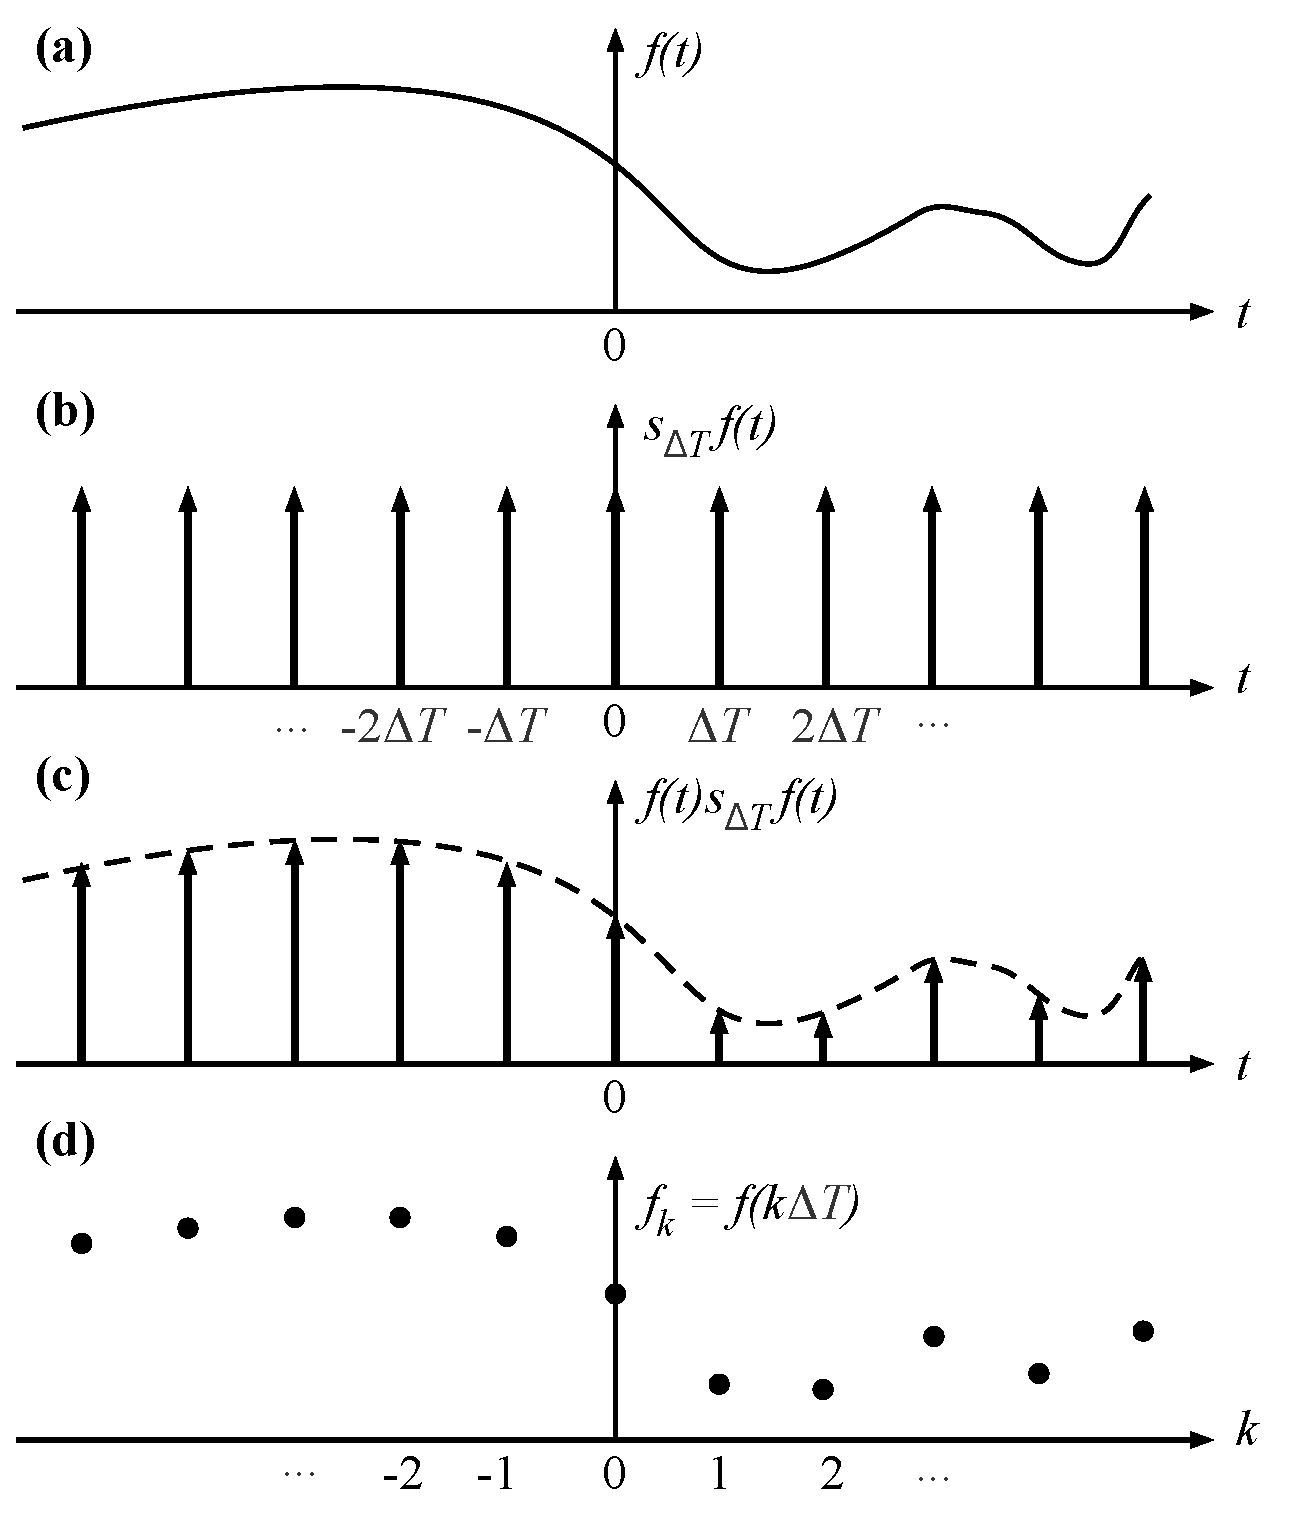
\includegraphics[width=0.65\textwidth]{figures/intro/sampling}
	\caption{冲激函数具有采样的能力,它可以简单地得到冲激位置处的函数值,所以函数$f(f)$的均匀采样可以定位为使用一个冲激串函数(b)与之相乘,这得到采样过后的函数(c),最终每个冲激位置处的采样值由加权后的冲激强度给出(d)}
	\label{f:intro-sampling}
\end{figure}

\begin{equation}
	\tilde{f}(t)=f(t)s_{\Delta T}(t)=\sum^{\infty}_{n=-\infty}f(t)\delta(t-n\Delta T)
\end{equation}

上述和式的每一个分量都是由在该冲激位置处$f(t)$的值加权后的冲激,如图\ref{f:intro-sampling}(c)所示。每个采样的值由加权后的冲激“强度”给出,我们可以通过积分得到它,即任意采样值$f_k$为:

\begin{equation}
	f_k=\int^{\infty}_{-\infty}f(t)\delta(t-k\Delta T){\rm d}t=f(k\Delta T)
\end{equation}

图\ref{f:intro-sampling}(d)显式了上述的采样结果,它由原始函数的等间隔采样而成。

为什么要用这么复杂的方式来表述函数采样呢?这是因为借助冲激函数的傅里叶变换以及卷积定理,我们可以得出采样定理,并进而指导我们对函数进行采样。

令$F(\mu)$表示连续函数$f(t)$的傅里叶变换,$\tilde{F}(\mu)$为采样后的函数$\tilde{f}(t)$的傅里叶变换,由卷积定理可得:

\begin{equation}
	\tilde{F}(\mu)=\Im\{\tilde{f}(t)\}=\Im\{f(t)s_{\Delta T}(t)\}=F(\mu)\star S(\mu)
\end{equation}

\noindent 其中,$\Im$符号表示傅里叶变换,$S(\mu)$为冲激串函数的傅里叶变换:

\begin{equation}
	S(\mu)=\cfrac{1}{\Delta T}\sum^{\infty}_{-\infty}\delta\bigg(\mu -\cfrac{n}{\Delta T}\bigg)
\end{equation}

可以看出,冲激串函数的傅里叶变换仍然为一个冲激串函数,这是一个非常重要的特性,由此我们可以得到采样后的函数$\tilde{f}(t)$的傅里叶变换为:

\begin{equation}
\begin{aligned}
	\tilde{F}(\mu)=&F(\mu)\star S(\mu)={\rm \int}^{\infty}_{-\infty}F(\tau)S(\mu-\tau){\rm d}\tau\\
	=&\cfrac{1}{\Delta T}{\rm \int}^{\infty}_{-\infty}F(\tau)\sum^{\infty}_{n=-\infty}\delta\bigg(\mu-\tau-\cfrac{n}{\Delta T}\bigg){\rm d}\tau\\
	=&\cfrac{1}{\Delta T}\sum^{\infty}_{n=-\infty}{\rm \int}^{\infty}_{-\infty}F(\tau)\delta\bigg(\mu-\tau-\cfrac{n}{\Delta T}\bigg){\rm d}\tau\\
	=&\cfrac{1}{\Delta T}\sum^{\infty}_{n=-\infty}F\bigg(\mu-\cfrac{n}{\Delta T}\bigg)
\end{aligned}
\end{equation}

\noindent 其中,上式的第一行使用了卷积的基本定义,即两个函数的卷积等于它们乘积的积分,仍然需要注意的是,上述卷积中的翻转函数$S(\mu)$会在每个$\tau$处作用于整个函数$F(\tau)$的定义域上,而由于$S$是一个冲激串函数,我们把$\cfrac{1}{\Delta T}$项提到外面,就产生了一个神奇的结果,即它在每个位置处将$F(\mu)$复制一次,而复制的间隔由$1/\Delta T$决定。很明显,虽然采样后的函数$\tilde{f}(t)$(在空间域)是离散的,但是其傅里叶变换$\tilde{F}(\mu)$(在频率域)却是连续的,因为它由$F(\mu)$的几个拷贝组成,而$F(\mu)$是连续的。

图\ref{f:intro-sampling-aliasing}显式了上述这种采样后函数的傅里叶变换图示,其中图\ref{f:intro-sampling-aliasing}(a)为原始连续带限函数$f(t)$的傅里叶变换,图\ref{f:intro-sampling-aliasing}(b)则表示采样后函数的傅里叶变换,如前所述,$1/\Delta T$是用于生成采样后函数的采样率。由此可以看出,为了保持对原始信号的重建能力,我们需要使用足够的采样率来保证$F(\mu)$的完整性,在图\ref{f:intro-sampling-aliasing}(c)中,采样率刚好能够保持$F(\mu)$,但在图\ref{f:intro-sampling-aliasing}(d)中,采样率低于保持不同$F(\mu)$拷贝的最小采样率要求。

\begin{figure}
	\sidecaption
	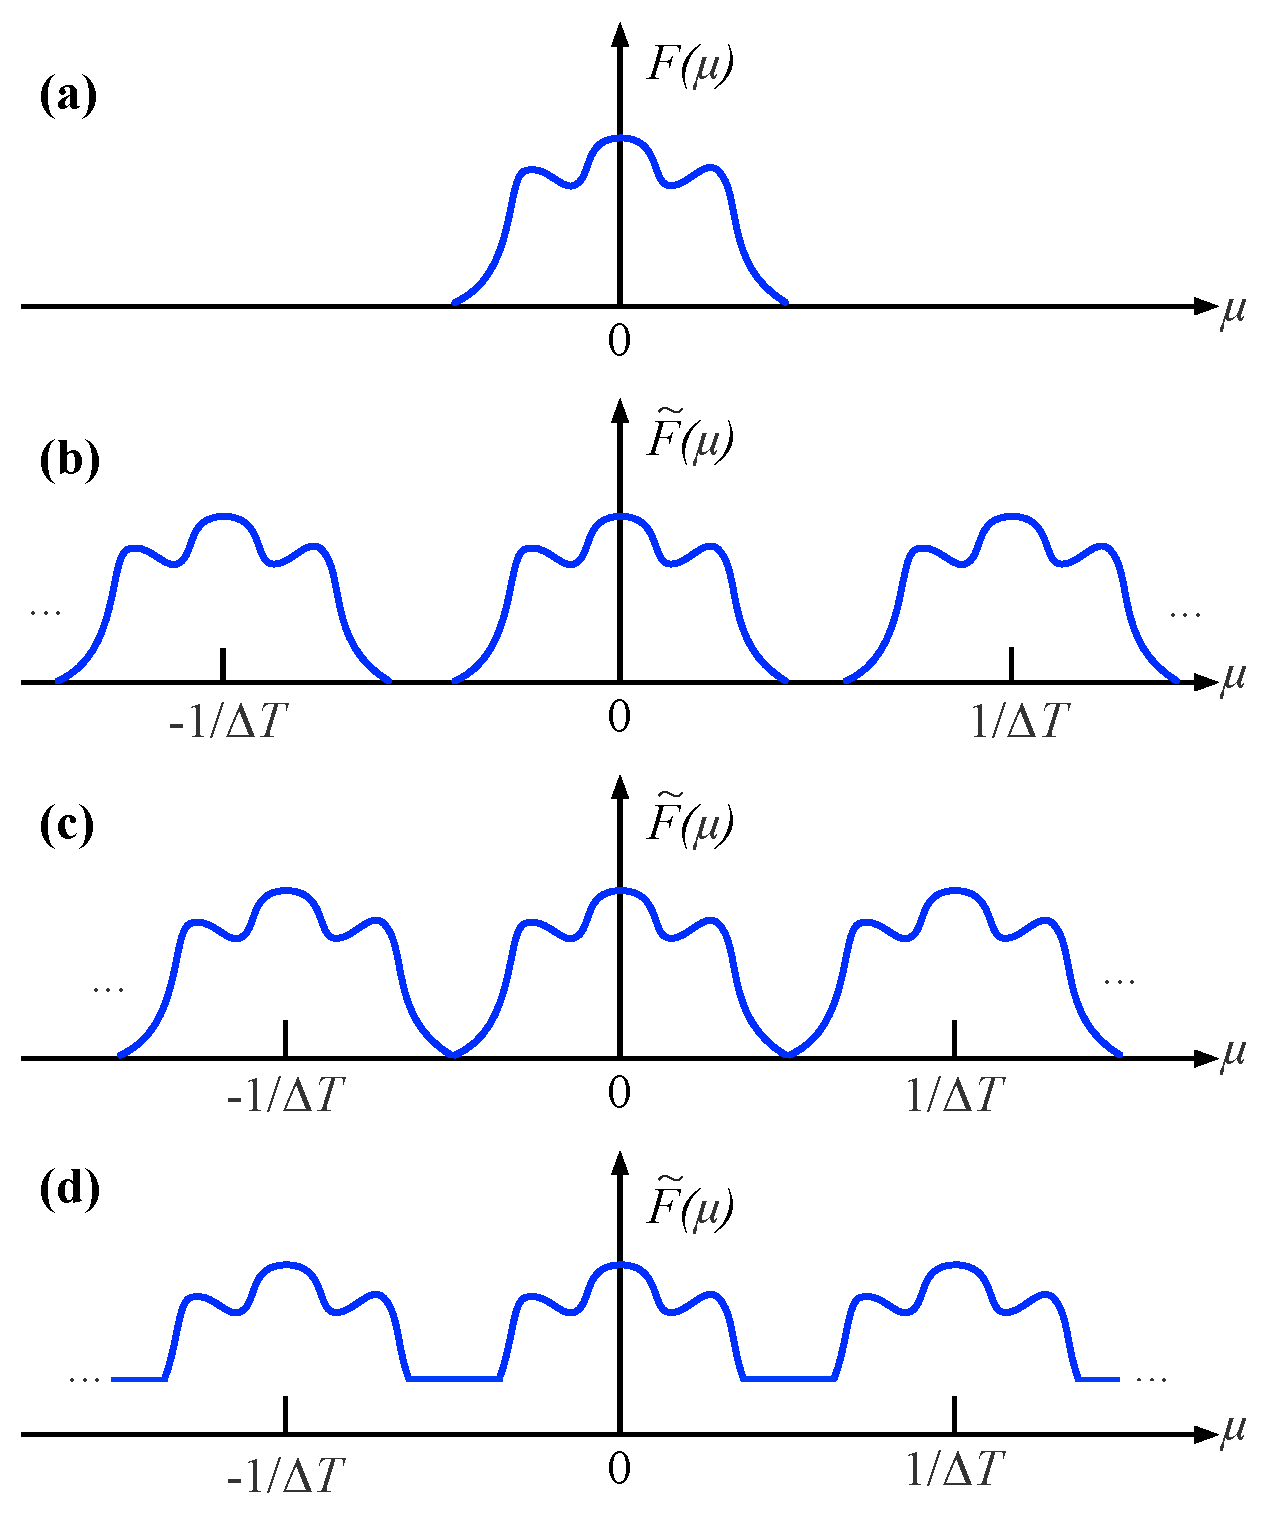
\includegraphics[width=0.65\textwidth]{figures/intro/sampling-aliasing}
	\caption{(a)为一个带限函数的傅里叶变换,(b)-(d)分别为过采样,临界采样和欠采样条件下采样后函数$\tilde{f}(t)$的傅里叶变换$\tilde{F}(\mu)$}
	\label{f:intro-sampling-aliasing}
\end{figure}

由此可知,当一个连续函数被采样成一个离散函数之后,其能够被重建为原函数的能力取决于采样点的密度(density of samples)\myindex{采样点的密度}{density of samples},或称为采样率(sample rate)\myindex{采样率}{sample rate}。根据采样理论(the sampling theorem)\myindex{采样理论}{the sampling theorem},对于一个带限函数$f(t)$,其最大的频率为$\mu_{\rm max}$,它能够完全被一系列以$1/(2\mu_{\rm max})$间隔采样的离散函数表示。换句话说,采样率必须大于或等于$2\mu_{\rm max}$采样点/秒,或者说对于一个采样率$f_s$,其离散函数能够被完美复原的条件是:$\mu_{\rm max}<f_s/2$。

当频率带宽$\mu_{\rm max}$太高(或者该函数完全不存在频率带宽),则这种不完美的复原导致的结果就是走样(aliasing)\myindex{走样}{aliasing}。这两个临界值$2\mu_{\rm max}$和$f_s/2$称作奈奎斯特采样率(Nyquist rate)\myindex{奈奎斯特采样率 }{Nyquist rate}和奈奎斯特频率(Nyquist frequency)\myindex{奈奎斯特频率}{Nyquist frequency}。由该采样定律定义的不等式条件称为奈奎斯特准则(Nyquist criterion)\myindex{奈奎斯特准则}{Nyquist criterion}。采样理论又称为奈奎斯特-香农采样定理(Nyquist–Shannon sampling theorem)\myindex{奈奎斯特-香农采样定理}{Nyquist–Shannon sampling theorem}以纪念Harry Nyquist和Claude Shannon对其的贡献。 

关于对离散函数的重建过程及其方法将在下一节讨论,采样的不足将导致走样的产生,本节最后将分析几种计算机图形学中涉及的一些比较重要的走样,通过对这些走样现象的分析和了解,将有助于更好地理解采样率对图像质量的影响。




\subsubsection{几何走样}
回到第\ref{sec:intro-sensor}节讨论的由于光栅化导致的三角形的走样,如图\ref{f:intro-aliasing-triangle}所示,对于光栅化,我们按照屏幕的分辨率对几何图形的可见性函数(visibility function)\myindex{可见性函数}{visibility function}进行采样,即采样点之间的间距为一个像素,采样点的位置为每个像素的中点。

可见性函数是一个连续函数,要想最终呈现很高质量的图像,必须要在图像上还原出很好的原始可见性函数,根据采样定律,必须要使用2倍于可见性函数最高频率的采样率。然而,三角形的可见性总是存在不连续,这种不连续性导致无限大的频率,从而使其傅里叶变换不存在有限的频率带宽,因此没有任何采样率可以阻止这种走样发生;另外根据傅里叶变换的条件,只有定义域在无限的时间域或空间域才能使其傅里叶变换具有有限的频率带宽。所以对于计算机图形学中有限的二维或三维空间域,走样现象是不可避免的。

这种由于对几何图形的可见性函数采样导致的走样称为几何走样(geometric aliasing)\myindex{几何走样}{geometric aliasing},它是计算机图形学中最严重的走样现象,因为整个场景图像的渲染都是根据物体表面的的位置来决定的,而每个像素点的位置都是光栅化阶段对物体几何形状的可见性函数来决定的。

虽然没有任何采样率可以有效地避免几何走样的存在(即完美地对可见性函数采样),但是我们仍然会寻求一些方法来减轻这种走样现象,其中比较流行的方法称为过采样(oversampling)\myindex{过采样}{oversampling},详见第\ref{sec:intro-resampling}节,这种方法本质上使用比图像分辨率更高的采样频率对原始可见性函数进行采样,然后使用这些采样点来重建像素对应的采样率下的函数值。这在3D渲染中相当于使用高于图像输出分辨率的频率渲染场景,然后将其缩放至输出分辨率,这个过程称为超采样(supersampling)\myindex{超采样}{supersampling}。本章后面第\ref{sec:intro-msaa}将详细讨论这种技术。




\subsubsection{着色走样}
着色走样(shader aliasing)\myindex{着色走样}{shader aliasing}发生于像素着色器中,它和纹理走样有点类似,也主要是由于像素着色器受限于屏幕分辨率所限导致的。然而不同的是着色走样主要是指,在着色器中对一些以分析的方式得到的连续函数的采样不足导致的走样,而不是对纹理的采样不足。

这类走样比较严重的例子是对粗糙度比较低的光泽表面的采样,由于表面低粗糙度导致其光泽分布范围更狭窄,如图\ref{f:intro-roughness}所示,从而导致光泽BRDF分布函数具有更高的频率,因而更容易导致走样。当对物体表面使用法线贴图后,这种走样现象更明显,因为法线导致物体表面的光泽具有更高的频率。

对于着色走样,其不可能通过后面第\ref{sec:intro-msaa}节介绍的MSAA技术解决,因为MSAA对于每个像素的着色只计算一次(但对Depth和Stencil值取多个采样点),所以它对着色走样没有任何影响;超采样(supersampling)虽然可以减少这类走样,但是其代价太高,并且提升效果不是很明显。如图\ref{f:intro-shader-aliasing}表示在有法线和光泽反射的情况下,三种不同方法的渲染结果。

\begin{figure}
\begin{fullwidth}
	\begin{subfigure}[b]{0.33\thewidth}
		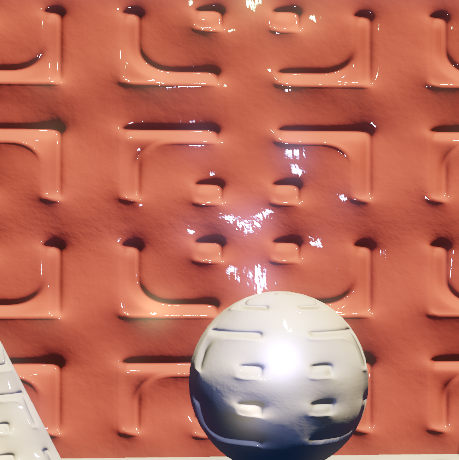
\includegraphics[width=1.\textwidth]{figures/intro/specaliasing_none}
	\end{subfigure}
	\begin{subfigure}[b]{0.33\thewidth}
		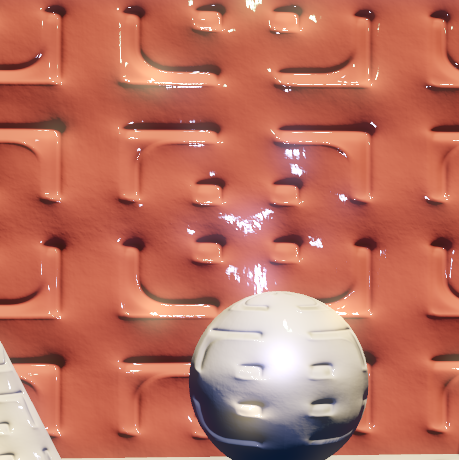
\includegraphics[width=1.\textwidth]{figures/intro/specaliasing_4xss}
	\end{subfigure}
	\begin{subfigure}[b]{0.33\thewidth}
		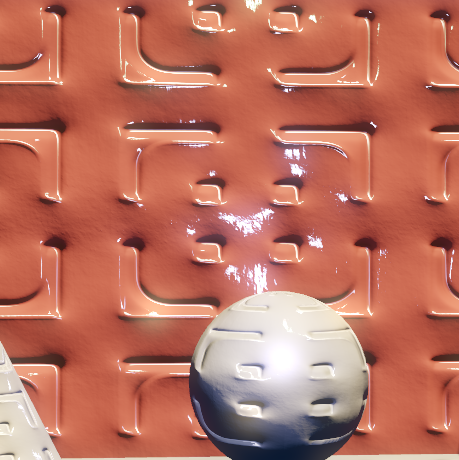
\includegraphics[width=1.\textwidth]{figures/intro/specaliasing_clean}
	\end{subfigure}
\caption{该图显示光泽和法线条件下,不同方法对着色走样的处理:左图正常绘制,走样现象比较严重,尤其注意在法线频率变化比较大的区域,信息丢失比较严重,中图使用4倍的超采样,右图使用一种直接基于法线计算光泽反射的方法,该方法能得到更好的结果(图片来自\cite{m:ApplyingSamplingTheorytoReal-TimeGraphics})}
\label{f:intro-shader-aliasing}
\end{fullwidth}
\end{figure}

对于渲染方程中由于粗糙度,法线以及其他相关因素导致的采样问题,比较有效的解决思路是,首先将这些参数融入到光照计算(例如后面讲述的微面元BRDF\myindex{微面元BRDF}{microfacet-BRDF}理论)中去,使这些“原始连续函数”更平缓,然后再对这些光照计算结果采样,这样的思路在本书后面的一些内容中有介绍。



\subsubsection{时间走样}
前面的例子都是对处于空间域的2个$(x,y)$或者3个$(x,y,z)$连续变量进行采样,然而在游戏或者电影动画渲染中,由于大量的物体处于运动状态,因此,对于另一个时间域的采样问题也特别突出。

时间走样(temporal aliasing)\myindex{时间走样}{temporal aliasing}出现于当物体在运动时,由于渲染帧率的限制使其对运动过程的采样不足导致的走样。游戏画面的渲染是根据帧率按较低的采样率对时间域进行采样,所以对于高速运动下的物品,其时间域的频率较高,很容易出现走样。其中一个比较经典的例子称为车轮效应(Wagon-wheel effect)\myindex{车轮效应}{Wagon-wheel effect},它使一个旋转的辐条车轮表现出不同的视觉效果,例如轮子可能看起来比实际更慢,或者看起来像静止一样,甚至沿着相反的方向旋转。

为了减轻时间走样,一种比较常用的方法称为运动模糊(motion blur)\myindex{运动模糊}{motion blur}。这种方法跟超采样一样,它依靠对时间域取更多的采样点,然后对其进行反走样,当然这种方法的计算成本很高。另一种更普遍的方法是针对当前帧渲染结果,生成一个速率缓存(velocity buffer)\cite{a:AReconstructionFilterforPlausibleMotionBlur}\myindex{速率缓存}{velocity buffer},然后使用这些方向在后处理阶段对其邻近的像素点执行插值计算,如图\ref{f:intro-motion-blur}所示。

\begin{figure}
	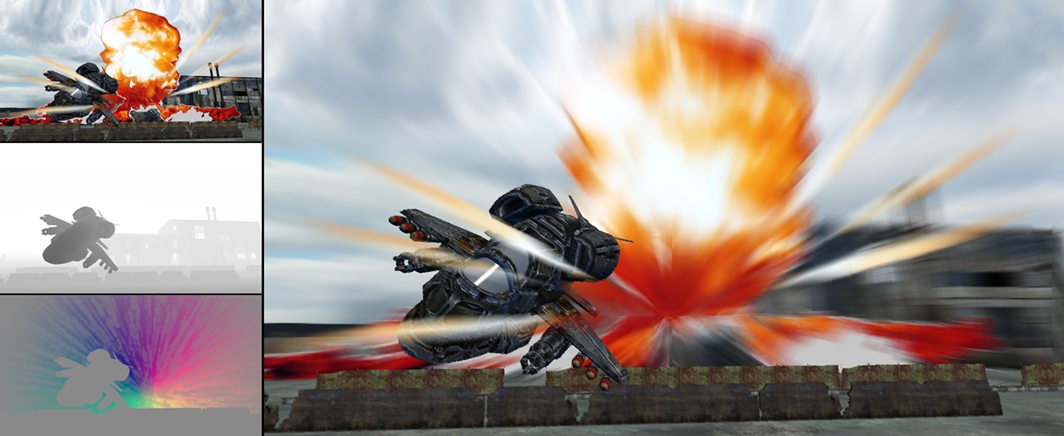
\includegraphics[width=1.\textwidth]{figures/intro/motion-blur}
	\caption{使用速率缓存实现运动模糊,图中左上表示当前帧的原始渲染结果,左中为深度缓存,左下为速率缓存,右图为最终结果}
	\label{f:intro-motion-blur}
\end{figure}



\subsection{重~~建}\label{sec:intro-reconstruction}
重建(reconstruction)\myindex{重建}{reconstruction}是指将采样后的离散函数还原为原始连续函数的过程,为了从一些离散的采样点还原为原始连续函数,必须对离散函数执行一个滤波器(filter)\myindex{滤波器}{filter}。“滤波”一词源于数字信号处理中,用于在频率域上接受(通过)或拒绝一定的频率分量。然而滤波器实际的概念非常复杂,根据滤波器是离散还是连续,以及被滤波器作用的函数是离散还是连续,滤波器的作用以及实现的结果都是不一样的。




\subsubsection{平~~滑}
根据卷积公式的特性,我们可以很容易想到它可以用来平滑函数$f$,然而不仅如此,根据卷积计算是作用在时间/空间域或者频率域,以及$f$和$g$是离散还是连续函数,它表现出来的功能特征和结果是不一样的,以下我们就分别来描述卷积的这些应用场景。

卷积计算最本质也是最直观的特征是平滑,它通过对$f$的每个点考虑该点周围一定范围内的值对该点的影响,来消除该点与周围环境的频率的快速变化。这在计算机图形学中运用时分广泛,大部分可能出现走样的地方,例如前面第\ref{sec:intro-sampling}节讨论的那些走样现象,都可以在采样之前对原始函数进行平滑,以减轻走样现象。这种滤波器称为反走样滤波器(anti-aliasing filter)\myindex{反走样滤波器}{anti-aliasing filter}。

这里举一个图像处理的例子,在图像处理中,常常考虑$f(x,y)$为一个具有一定分辨率的图像,$g(x,y)$为一个$m\times n$的矩形,其分辨率通常小于或等于$f(x,y)$的分辨率,假设$m=2a+1$且$n=2b+1$,其中$a,b$为正整数,则式\ref{eq:intro-conv}变为:

\begin{equation}\label{eq:intro-convolution-2}
	g(x,y)\star f(x,y)=\sum^{a}_{s=-a}\sum^{b}_{t=-b}g(s,t)f(x-s,y-t)
\end{equation}

可以看出,卷积的意义相当于使用一个$m\times n$的模板$g$,以它的中心从$f$ 的每一个像素点经过,对于每一个像素点,分别计算模板上对应位置的两个函数乘积的和,如图\ref{f:intro-conv}所示,其卷积输出为一个新的与$f$分辨率相同的图像。

\begin{figure}
\sidecaption
	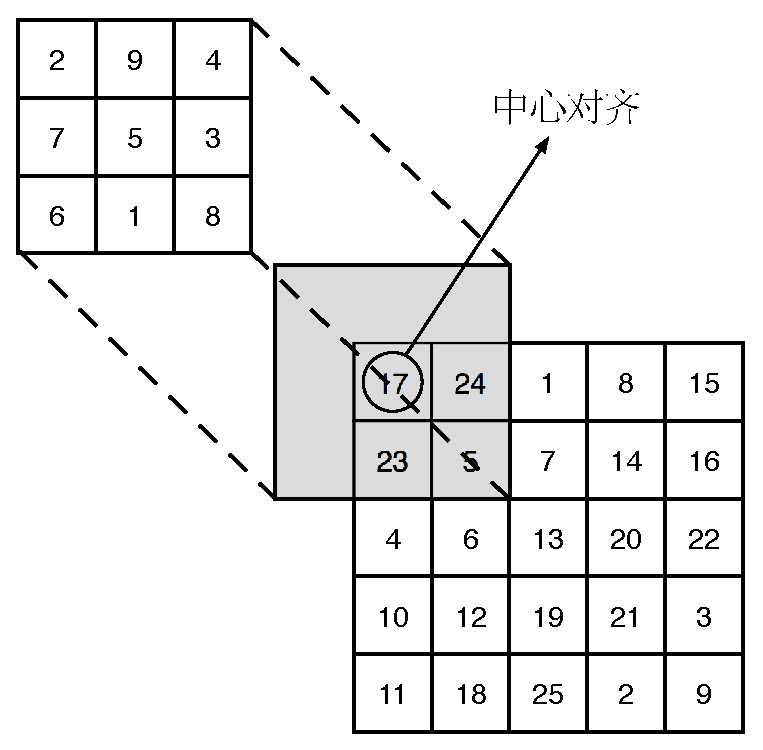
\includegraphics[width=.5\textwidth]{figures/intro/conv}
	\caption{在图像处理中,卷积的意义相当于使用一个蒙板遍历每一个像素点,分布计算蒙板内所有乘积的和,GPU中纹理过滤相关的技术都是通过卷积的方式实现}
	\label{f:intro-conv}
\end{figure}



\subsubsection{重~~建}
除了平滑,借助卷积的特性还可以实现将离散函数还原为原始连续函数,卷积的这种运用称为重建滤波器(reconstruction filter)\myindex{重建滤波器}{reconstruction filter}。重建的操作表现为用一个无限连续的$g$作用于采样后离散的$f$,然而为了直观理解重建的过程,我们需要首先从频率域以及采样定理说起。

前面已经介绍过采样定理相关的内容,设$\tilde{F}(\mu)$为对$f(t)$采样后的离散函数$\tilde{f}(t)$的傅里叶变换,如图\ref{f:intro-reconstruction}(a)所示,为了使$f(t)$能够被完美重建,首先需要保留$\tilde{F}(\mu)$所有的频率,在本例子中使用了一个高于奈奎斯特采样率的频率进行采样。如果能够从$\tilde{F}(\mu)$中包含的这个函数的拷贝的周期序列中分离出$F(\mu)$的一个拷贝,那么我们就可以从采样后的版本恢复$f(t)$。

\begin{figure}
\sidecaption
	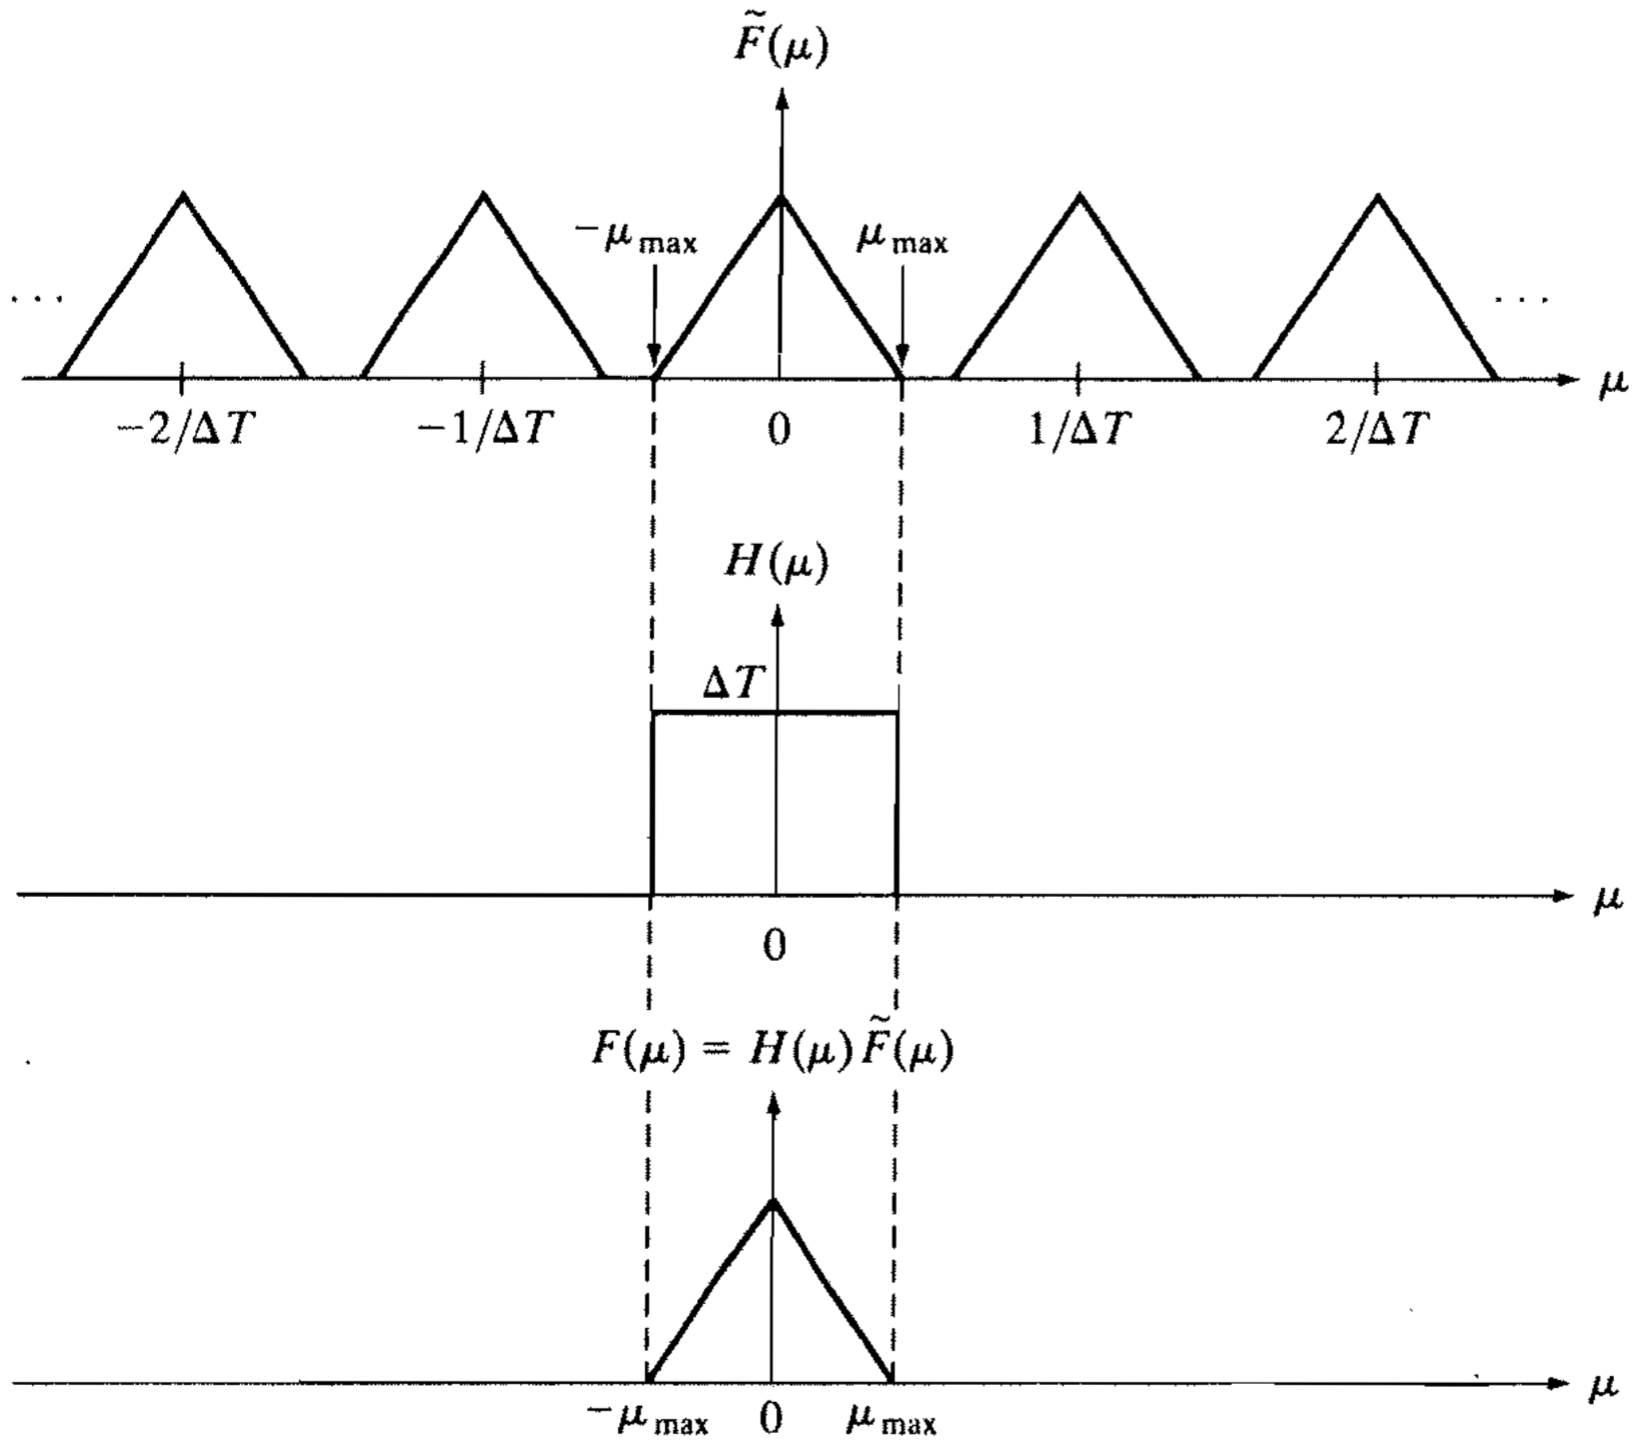
\includegraphics[width=.65\textwidth]{figures/intro/reconstruction}
	\caption{盒状滤波器通常用来在频率域对信号进行重建}
	\label{f:intro-reconstruction}
\end{figure}

为了从原理上了解如何从$\tilde{F}(\mu)$复原$F(\mu)$,在图\ref{f:intro-reconstruction}(b)中$H(\mu)$的定义如下:

\begin{equation}
	H(\mu)=\begin{cases}
		\triangle T & -\mu_{\max}\leq\mu\leq\mu_{\max}\\
		0           & \text{其他}
	\end{cases}
\end{equation}

\noindent 当乘以图\ref{f:intro-reconstruction}(a)中的周期序列时,该函数就隔离了以原点为中心的一个周期,然后通过$H(\mu)$和$\tilde{F}(\mu)$相乘得到$F(\mu)$:

\begin{equation}\label{eq:intro-reconstruction}
	F(\mu)=H(\mu)\tilde{F}(\mu)
\end{equation}

\noindent 一旦得到了$F(\mu)$,就可以通过傅里叶反变换来复原$f(t)$:

\begin{equation}
	f(t)={\rm \int}^{\infty}_{-\infty}F(\mu){\rm e}^{j2\pi\mu t} {\rm d}\mu
\end{equation}

\noindent 以上这些公式从理论上证明了,以函数包含的最高频率的两倍的速率采样得到的函数的样本,来恢复一个带限函数是可能的。

上述的函数$H(\mu)$称为一个低通滤波器(low-pass filter)\myindex{低通滤波器}{low-pass filter},因为它通过频率范围低端的频率,并且消除所有较高的频率。所以要想完美复原原始函数,原始函数$(f(t))$必须是带限函数。

对式\ref{eq:intro-reconstruction}利用卷积定理,可以在空间域得到等价的结果,即:

\begin{equation}
	f(t)=\Im^{-1}\{F(\mu)\}=\Im^{-1}\{H(\mu)\tilde{F}(\mu) \}=h(t)\star\tilde{f}(t)
\end{equation}

\noindent 可导出$f(t)$的如下空间域表达式(此处略去证明过程,请参考\cite{b:DigitalImageProcessing}等相关书籍):

\begin{equation}\label{eq:intro-reconstruction-1}
	f(t)=\sum^{\infty}_{n=-\infty}f(n\triangle T) {\rm sinc}[(t-n\triangle T)/\triangle T]
\end{equation}

\noindent 这相当于对离散函数使用一个辛克函数(sinc function)\myindex{辛克函数}{sinc function}(如图\ref{f:intro-sinc}所示)的卷积,辛克函数的定义如下:

\begin{equation}
	{\rm sinc}(x)= \cfrac{\sin (\pi x)}{\pi x}
\end{equation}

\noindent 这并不奇怪,因为盒装滤波器$H(\mu)$的傅里叶反变换就是一个辛克函数。

\begin{figure}
\sidecaption
	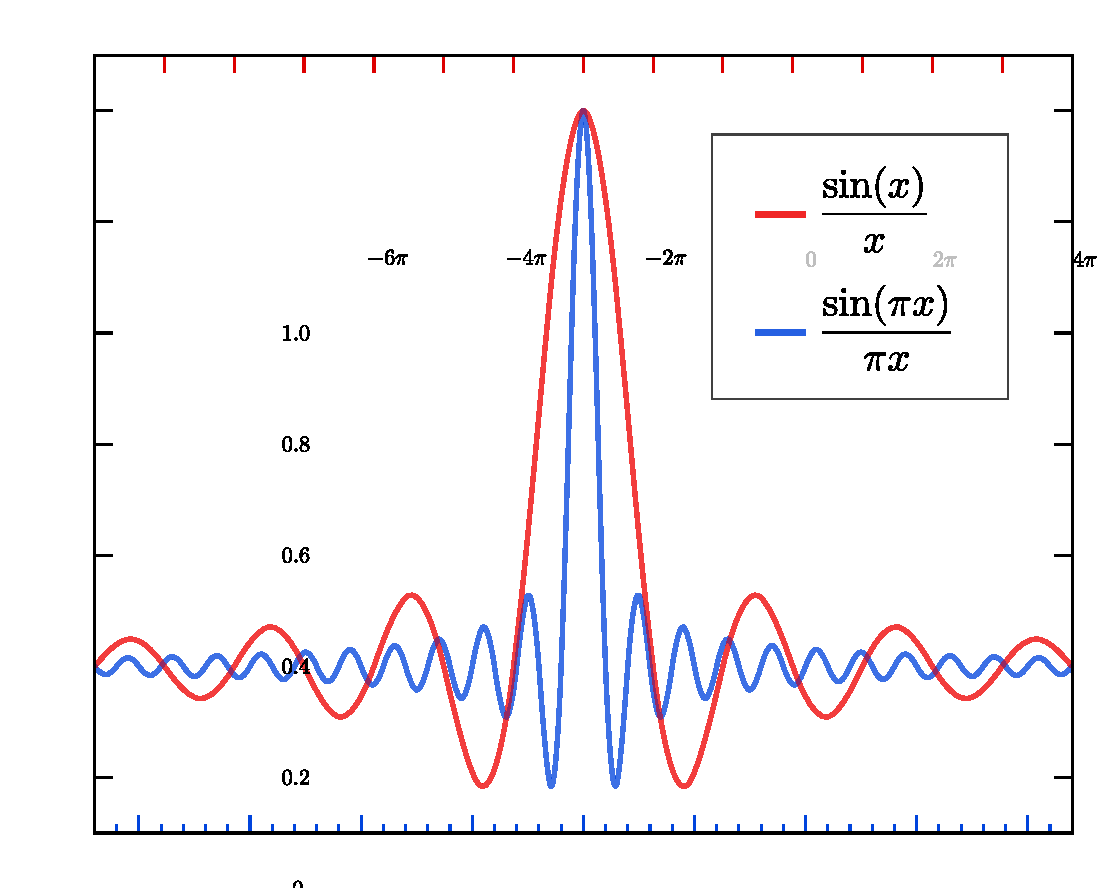
\includegraphics[width=.65\textwidth]{figures/intro/sinc}
	\caption{蓝色曲线表示归一化的辛克函数,而红色曲线表示未归一化的辛克函数,在计算机图形学中一般使用归一化的版本(图片来自Wikipedia)}
	\label{f:intro-sinc}
\end{figure}

我们不禁要问,卷积主要用来平滑一个离散或者连续函数,那它是怎样实现这种类似于在样本点之间插值的效果的呢?这里主要是由于辛克函数是在无限空间连续的,所以当它划过$\tilde{f}(t)$上的每一点时,会在辛克函数的整个定义域上求积分,因为积分值是一个标量,即该点的卷积总是可能具有一个值,并且这个值其实是考虑$\tilde{f}(t)$所有点的平滑效果而得来的,因此它能完美还原$f(t)$,同时实现了使用卷积来重建一个离散函数。当卷积被这样使用时,称之为重建过滤器(reconstruction filter)\myindex{重建过滤器}{reconstruction filter}。

在图像处理中,重建过滤器主要有两个用途:第一种为上面讲述的从一个采样过的离散函数重建原始连续函数,另一种称为重采样(见第\ref{sec:intro-resampling}节),即在纹理被缩小或者放大时,调整图像的分辨率。这两种场景本质上都是把滤波器看做一种计算某个特定的点的插值的工具,即我们并不需要对一张图像全部像素点做卷积计算,而是找出另外一些当前这些采样点之外的点的值。

然而,式\ref{eq:intro-reconstruction-1}要求样本间的内插有无限多项,在实际中,这意味着我们必须找到一种样本间内插有限的近似方法,在图像处理中使用的主要内插方法是最近邻法,双线性法和双三次内插法,这些插值方法将在下一节讨论。





\subsection{重采样}\label{sec:intro-resampling}
在渲染场景的时候,程序会大量使用预先采样的数据,如图像,或者场景的某些离散的表示空间结构数据等。这些数据都是具有一定的分辨率(或者是按一定的采样率生成的数据),当程序中需要在不同分辨率下使用这些数据时(例如摄像机靠近或者远离表面导致纹理被放大或者缩小),我们需要对这些离散的数据进行重采样(resampling)\myindex{重采样}{resampling},以生成一个具有不同分辨率的数据。以下我们主要以GPU中对纹理的采样分析分辨率转换的问题。

当摄像机靠近物体表面时,即发生放大操作(magnification)\myindex{放大操作}{magnification},这使摄像机能看到更多细节,它要求对原始函数使用更高的采样率采样。如图\ref{f:intro-magnification}所示,这要求生成更多的采样点,根据上一节讲述的内容,我们只需要对于离散的图像提供一个滤波器,便可以对任意点进行插值。

\begin{figure}
\begin{fullwidth}
	\includegraphics[width=\thewidth]{figures/intro/magnification}
	\caption{左图的原始经过采样的离散信号,当摄像机靠近物体上需要对信号进行放大操作(图片来自\cite{b:rtr})}
	\label{f:intro-magnification}
\end{fullwidth}
\end{figure}

然而,正如前面提到的,辛克函数要求样本间的内插值有无限多项,所以我们必须使用一些近似方法来进行插值计算。最简单的方法是最近邻插值(nearest-neighbor interpolation)\myindex{最近邻插值}{nearest-neighbor interpolation},它采用像素复制的放大操作。例如,将一幅图像放大两倍,我们可以复制每一列,这会在水平方向上将图像尺寸放大一倍;然后复制这幅放大后图像的每一行,在垂直方向上将图像尺寸放大一倍。相同的步骤可用于任意整数倍放大图像。最近邻内插法实际上是对图像使用一个盒式过滤器(box filter)\myindex{盒式过滤器}{box filter},如图\ref{f:intro-Piecewise_constant}所示。

\begin{figure}
\sidecaption
	\includegraphics[width=.45\textwidth]{figures/intro/Piecewise_constant}
	\caption{最近邻内插法直接选择离重建点最近的样本值作为内插值(图片来自Wikipedia)}
	\label{f:intro-Piecewise_constant}
\end{figure}

双线性插值(bilinear interpolation)\myindex{双线性插值}{bilinear interpolation}法则分别基于采样点的位置在$X$和$Y$轴上线性地插值,如图\ref{f:intro-BilinearInterpolation}所示。双线性插值法本质上对图像执行一个三角形过滤器(triangle filter)\myindex{三角形过滤器}{triangle filter}或称为篷形过滤器(tent filter)\myindex{篷形过滤器}{tent filter}。

\begin{figure}
\sidecaption
	\includegraphics[width=.45\textwidth]{figures/intro/BilinearInterpolation}
	\caption{双线性插值法分别基于采样点的位置在$X$和$Y$轴上线性地插值(图片来自Wikipedia)}
	\label{f:intro-BilinearInterpolation}
\end{figure}

双线性插值法仅仅考虑采样点周围的4个$2\times 2$像素点,双三次内插法(bicubic interpolation)则考虑周围16个$4\times 4$像素点,可以给出更平滑的插值结果(最近邻插值法和双线性插值法都会使还原的函数具有导数不连续的点,即导致非常高的频率变化,从而导致走样比较严重)。双三次内插法使用的滤波器函数如下:

\begin{equation}
	W(x)=\begin{cases}
		(a+2)|x|^{3}-(a+3)|x|^{2}+1 & $for $|x|\leq 1 \\
		a|x|^{3}-5a|x|^{2}+8a|x|-4a & $for $1<|x|<2   \\
		0 & 其他
	\end{cases}
\end{equation}

\noindent 这里$a$通常取值-0.5或者-0.75,注意$W(0)=1$,对于所有非0整数$W(n)=0$。双三次函数具有如图\ref{f:intro-bicubic}所示的形状。

\begin{figure}
\sidecaption
	\includegraphics[width=.6\textwidth]{figures/intro/bicubic}
	\caption{双三次内插法考虑周围16个$4\times 4$像素点,可以给出更平滑的插值结果(图片来自Wikipedia)}
	\label{f:intro-bicubic}
\end{figure}




\subsection{全屏反走样}\label{sec:intro-msaa}
 在第\ref{sec:intro-sampling}节讨论了几种形成走样的原因,其中的几何走样和着色走样这两种比较明显的走样是和分辨率有关的,所以如果我们能够从像素着色器(pixel shader)来解决走样的问题,或许我们能够解决所有由于分辨率带来的走样\footnote{注意,前面提到过着色走样并不能通过本节所讲述的MSAA技术减轻走样,本节稍后将会分析其原因。}。本节基于屏幕空间的反走样技术正是基于这样的思路,并且它通常是由硬件在渲染管线中直接实现的反走样技术,因此不对任何具体渲染实现有什么影响。

在开始讨论具体的全屏反走样技术之前,首先我们应该思考的是,对于固定的屏幕分辨率(相当于固定的采样率),其反走样的思路是什么。通过前面对采样及滤波器等知识的学习,我们知道走样是一个采样问题,它不能通过任何技术手段在采样之后消除这种由采样不足导致的走样。那么走样是什么,走样是由于采样率低导致傅里叶变换的高频部分没有被覆盖,从而使相邻的采样点之间出现比较大的差值。所以,对于固定采样率的前提下,我们能做的事情就是对原始函数进行平滑,消除原始函数的高频部分,而这可以通过低通过滤器来实现(回想第\ref{sec:intro-reconstruction}节滤波器的主要功能是通过卷积实现平滑)。

然而,在渲染中,我们通常并不能对原始函数进行平滑,一方面存储这样的原始函数(例如几何图形的可见性函数)需要大量的内存;另一方面,平滑是一个相对的概念,例如一个图像数据的频率对于$1920\times 1200$的分辨率来说是平滑的,但是它对于$1024\times 640$的分辨率来说频率带宽仍然太宽。这就是为什么纹理缩小时需要使用多级纹理(mipmap)\myindex{多级纹理}{mipmap}技术而不是直接从原始图像进行缩放。

根据以上这些分析,过采样(oversampling)\myindex{过采样}{Oversampling}就是一种针对特定分辨率的反走样技术,它通过使用一个比输出分辨率略高的采样率对原始函数进行采样,并对这个高分辨率的样本函数使用滤波器进行平滑,然后对这个高分辨率的样本函数进行重采样得到输出分辨率的图像。

过采样又称为超采样(supersampling)\myindex{超采样}{supersampling},它是一种对每个像素点计算多个子采样点(subsamples)\myindex{子采样点}{subsamples}的反走样技术。其最简单的形式称为全屏反走样(full-scene antialiasing,FSAA)\myindex{全屏反走样}{full-scene antialiasing},FSAA对场景以一个更高的分辨率进行渲染,然后对相邻的采样点取平均值得到最终图像,例如对于一个$1000\times 800$分辨率的图像,首先使用$2000\times 1600$的分辨率对场景进行渲染,然后对每个$2\times 2$的样本面积求平均值得到最终图像。这种技术的特点是实现非常简单,但是其计算成本很高,每一个子采样点都需要被使用完整的渲染管线进行着色。

\begin{figure}
\begin{fullwidth}
	\includegraphics[width=\thewidth]{figures/intro/sampling-pattern}
\caption{根据实现不同,FSAA对子样本点使用不同的采样模式(图片来自Wikipedia)}
\label{f:intro-Supersampling-pattern}
\end{fullwidth}
\end{figure}

对于FSAA,需要注意的是,可以对每个像素范围内的子采样点采用不同的分布,图\ref{f:intro-Supersampling-pattern}介绍了其中几种采样模式\footnote{关于采样模式,我们将在第\ref{chp:mc}章介绍更多的细节。}(sampling pattern)\myindex{采样模式}{sampling pattern},不同的采样模式具有不同的优点,例如RGSS对像素格子按规则的采样模式进行渲染,然后将样本进行旋转,这样得到的结果使得接近水平线的变化更加平坦,实际上,\cite{a:Jaggededges:whenisfilteringneeded?}指出人的眼睛对接近水平或垂直直线的走样更敏感,而对$45^{o}$左右直线的走样敏感度是最低的;Nvidia的高分辨率反走样(high-resoulution antialiasing,HRAA)\footnote{参见:\url{http://www.evga.com/articles/41.asp}}使用Quincunx的采样模式,它对每个像素点使用两个子采样点,但是使用Quincunx的分布模式,使得每个像素可以使用周围的4个(一共5个点)相邻的子采样点进行平均求值。当然这里只列出少数几种采样模式\footnote{参见:\url{https://en.wikipedia.org/wiki/Supersampling}。}。

超采样技术对每个子采样点的着色,深度及位置等都需要进行单独的计算。对于由几何图形光栅化导致的走样,实际上我们只需要对其可见性函数进行采样即可,即是说我们可以将可见性函数从着色当中分离出来,这样对于每个像素点只需要计算一次着色(即执行一次像素着色器),这样将大大减少反走样的计算量。基于这样思路的反走样技术称为多重采样反走样(multisample antialiasing,MSAA)\myindex{多重采样反走样}{multisample antialiasing}。然而其代价是由于每个像素的颜色只计算一次,因此它不能实现着色走样的反走样,这仍然需要借助多级纹理等技术来实现。

MSAA需要借助图形API的光栅化技术来实现,在图形渲染管线(见第\ref{chp:pipeline}章)的光栅化阶段,光栅化器根据输入的几何图形的顶点,按照输出分辨率将几何图形光栅化成一个个像素点,然后对每个像素点执行一个像素着色器以计算该像素颜色,深度,模板值,其中像素着色器只计算颜色值,而深度值由光栅化器计算,模板值则应用程序对图形接口的调用来决定。而在一个实现MSAA的光栅化器,它会对每个像素生成多个子采样点,并计算每个子采样点的深度和模板值,而对于颜色值,光栅化器对每个像素只调用一次像素着色器,然后将计算结果复制给每个子采样点。

\begin{figure}
	\includegraphics[width=1.\textwidth]{figures/intro/msaa}
	\caption{DirectX 11中MSAA的实现,其中$\cdot$为子采样点的位置,$\bigcirc$为几何图形覆盖的子采样点,$\diamond$为像素着色器执行颜色计算的位置(图片来自MSDN)}
	\label{f:intro-msaa}
\end{figure}

图\ref{f:intro-msaa}为DirectX 11中MSAA的实现,对于每个通过深度和模板测试的子采样点,其深度和模板值将被写入到缓冲区,该子采样点的颜色值由像素着色器计算,该颜色将被乘以该像素点的覆盖率,覆盖率是由几何图形所占区域的子采样点与总采样点之比。

在上述的光栅化过程中,像素着色器根据像素点中心的位置从纹理采样,以计算该像素的颜色值,然而如果几何图形只占据像素点的一小部分,则中心点不会被覆盖到,从而导致从纹理中不正确的位置获得颜色值。为了保证颜色计算的正确性,这个像素着色器使用的采样位置可以被调整到覆盖区域中某个点的位置,这种技术称为质心采样(centroid sampling)\myindex{质心采样}{centroid sampling},或者质心插值(centroid interpolation)\myindex{质心插值}{centroid interpolation}。对于一个被几何图形覆盖的像素点,它首先从像素中心点开始寻找,如果中心点没被几何图形覆盖,则一次向外延伸直到找到一个被覆盖的子采样点,该点的位置将作为最终像素着色器对纹理采样的位置。

MSAA相对于超采样大大减少了计算量(每个像素着色器只执行一次计算),然而MSAA并没有减少内存占用,CSAA\cite{m:CoverageSamplingAntialiasing}则进一步将像素点的覆盖率从颜色/深度/模板值当中分离出来,使其内存占用和数据传输的宽度占用都得到降低。

\begin{figure}
\sidecaption
	\includegraphics[width=0.55\textwidth]{figures/intro/sample_coverage}
	\caption{一个$16\times$CSAA的颜色和覆盖率存储结构,该设置使用4个子采样点,但是使用16个位置来计算其覆盖率,使得覆盖率数据更精准}
	\label{f:intro-sample-coverage}
\end{figure}

如图\ref{f:intro-sample-coverage}所示,除了MSAA中的子采样点,CSAA还使用了一个二进制结构的数组蒙板(bit mask)表示覆盖率,这个覆盖率比子采样点具有更高的分辨率,在光栅化阶段,光栅化其首先投影几何图形到该蒙板以计算覆盖率,然后对子采样点进行采样计算深度,模板及颜色值,其中计算颜色值的时候其覆盖率直接由该蒙板提供。这样使得更少的子采样点可以得到更精准的覆盖率,而原本这需要更多的子采样点来存储这些数据,而每个子采样点存储深度,模板及颜色值,所以在存储占用及数据传输带宽占用方面都是很大的。

关于覆盖率与深度,模板及颜色值的分离,其思路来源于\cite{a:TheA-bufferanAntialiasedHiddenSurfaceMethod}中的A-buffer技术,图形学中还存在大量从分离覆盖率着手的解决方案。本节仅对全屏反走样技术做基本的介绍,更多的反走样技术还涉及与渲染方法(例如延迟着色)结合起来工作,所以我们需要在接触相关的概念之后才能进行深入地学习,后面还会更深入地讨论各种各样的反走样技术。




\section{基于物理的渲染}
我们已经知道了光在空中传播及与表面交互的一些度量,并且我们知道最终摄像机收集每个像素点的辐射亮度$L$,以及怎样减轻由于屏幕分辨率的限制导致采样时走样的现象。虽然这一切建立在物体表面为理想光滑平面的基础之上,但是我们通过这样简化的模型很好地讨论了计算机图像渲染的逻辑和过程。当物体表面变得复杂时,渲染方程的计算将发生变化,但是这个逻辑框架是不会变化的。所以在理解了这些渲染过程及逻辑之后,本节就开始讨论实际渲染中,光与表面交互更复杂的情形,这也是计算机图形学关于渲染部分最需要关心的重要知识。

本节我们将建立这些光与表面复杂交互过程的数学模型,各种渲染方法的实现基本上都是基于这些光照数学模型的。当然不同级别的引擎对这些数学模型有不同级别的近似,在光传输过程中的各个环节也可能使用不同的近似方法处理(正如本书将介绍的各种全局光照算法),但是本节介绍的基础知识几乎是所有全局光照模型的基础。

由于渲染方程的复杂性,以及硬件性能的限制,早期的工业运用中(甚至处于离线渲染的电影行业)大都使用一些非常近似的模型,这些模型能够产生比较理想的效果,然而这些图像结果却不是物理上正确的。所谓物理上正确的,主要指光在场景中的传输保持能量守恒(本节后面将会讲述更多关于基于物理渲染的特征)。基于物理的渲染能够使渲染结果更能够接近物理世界的品质。

自从2012年Burley的论文\cite{a:PhysicallyBasedShadingatDisney}之后,游戏行业已经开始广泛采用基于物理的渲染,并在之后几年的各种技术会议上,业界各大主流游戏引擎都纷纷展示了它们基于物理渲染的效果和品质。所以本书中大多数解决方案都是基于物理的。




\subsection{双向反射分布函数}\label{sec:intro-BRDF}
当一个表面绝对光滑时,一束入射光将按照反射定律在相应的方向上被反射,以及按照折射定律在相应的方向上被折射。对于除这两个方向以外的方向,将得不到任何来自这束入射光的光照。

我们的世界显然不是这样的,每种物体表面都有着各种不同的粗糙度,这使得光线照射到一个表面后,可以沿着不同的方向看到这些反射或折射的光。这是由于在物理世界中,每个光子入射到一个特定的微观表面上,这些微观表面由于材质的粗糙度而朝向多个不同的方向,在这个微观表面上,光与物体的交互仍然遵循反射定律和折射定律。

\begin{figure}
\sidecaption
	\includegraphics[width=0.5\textwidth]{figures/intro/surface-roughness}
	\caption{在数字图像的世界,每一个像素点其实对应着具有不同粗糙度的表面,这个表面位于微观尺寸,它小于一个像素的尺寸但是,但是大于光的波长,但这个尺寸我们很难通过几何模型来模拟(图片来自Wikipedia)}
	\label{f:intro-surface-roughness}
\end{figure}

然而数字图像的世界可不是这样,由于物理世界被像素化为一个离散的数字图像,一方面对于小于一个像素的微观尺寸,我们通常无法用一种真实的几何模型表述其微观结构,如图\ref{f:intro-surface-roughness}所示;另一方面,即使对于宏观的尺寸,对于较远的场景,一片较大的区域将被投射到一个单一的像素点上,而这片较大的区域拥有不同的粗糙度,使得摄像机可以从各个不同的角度看见它。

那么我们怎样表示不同物体表面的这种粗糙度性质呢?首先我们从结果上来分析,由于这种微观结构的存在,它使得来自每个方向的每束光在表面的各个方向上具有一个特定的分布函数(回想第\ref{sec:intro-materials}节中讲述材质时物体微观结构上的粗糙度使得一束光在一个像素点上可以沿多个不同的方向折射或反射),这个分布函数可能由多种不同的因素决定,例如粗糙度,是否是金属结构等等,但是只要找到这个分布函数,便能够有效地计算光与表面的交互。

在数学上,用一个双向反射分布函数(bidirectional reflectance distribution function,BRDF)\cite{a:DirectionalReflectanceandEmissivityofanOpaqueSurface}\myindex{双向反射分布函数}{bidirectional reflectance distribution function}来表示物体表面的反射。它表示反射方向上的辐射亮度增量与入射方向辐射照度增量的比率:

\begin{equation}\label{eq-intro-brdf}
    f_r(\omega_i,\omega_r)= \cfrac{{\rm d}L_r(\omega_r)}{{\rm d}E_i(\omega_i)}= \cfrac{{\rm d}L_r(\omega_r)}{L_i(\omega_i)\cos\theta_i {\rm d}\omega_i}
\end{equation}

其中,$\omega_i$是入射光方向,$\omega_r$表示观察方向,$\theta_i$为入射光方向与表面法线$\mathbf{n}$的夹角 如图\ref{f:intro-brdf}所示。由于在球面坐标系中,一个方向可以用一个方位角(azimuth angle)\myindex{方位角}{azimuth angle}$\phi$和一个顶点角(zenith angle)\myindex{顶点角}{zenith angle}$\theta$表示,因此整个BRDF函数具有4个变量。BRDF函数的单位为$sr^{-1}$,其中$sr$为立体角。直观上讲,BRDF的值表示入射光方向单位立体角的能量在反射方向上反射的比率。

\begin{figure}
\sidecaption
	\includegraphics[width=0.5\textwidth]{figures/intro/BRDF_Diagram}
	\caption{BRDF函数由2个方向组成,具有4个变量,它本质上指明了每个方向的入射光在各个方向上的反射光分布}
	\label{f:intro-brdf}
\end{figure}

这里使用微分方程的原因是,对于非${\rm d}\omega_i$方向的辐射照度,其与$f_r(\omega_i,\omega_r)$无关,但是仍然可能影响$L_r(\omega_r)$的值,然而${\rm d}E_i(\omega_i)$只影响${\rm d}L_r(\omega_r)$的值。即整个$L_r(\omega_r)$是由各个入射方向的光照反射的结果。

所以,给定BRDF函数,便可以求出该点处沿观察方向的辐射亮度,其值为入射方向的辐射亮度乘以BRDF函数,再乘以一个余弦因子之后,沿该点法线方向半空间的积分,即:

\begin{equation}\label{eq:intro-reflectance}
	L_r(\omega_r)={\rm \int}_{\Omega}f_r(\omega_i,\omega_r)\otimes L_i(\omega_i)\cos\theta_i {\rm d}\omega_i
\end{equation}

\noindent 其中$\otimes$标记表示按RGB分量相乘,因为辐射照度$E$和辐射亮度$L$都是RGB矢量,所有$f_r$仍然表示为一个由RGB三个分量构成的矢量。方程\ref{eq:intro-reflectance}又称为反射方程(reflectance equation)\myindex{反射方程}{reflectance equation}。




\subsubsection{双向表面散射反射分布函数}
在第\ref{sec:intro-materials}节讨论材质时讲过,对于非金属不透明\footnote{透明物体由于物体内部材质连续,光折射后在物体内部的传播方向不受改变,然后从物体表面的相反方向射出。}物体,当光进入物体内部(而不仅仅是表面)时,这些折射的光会由于物体内部结构的不连续导致光沿着不同的方向继续散射,最终一部分光会被吸收,而剩下的光会从表面的另一个不同的地方散射出来,如图\ref{f:intro-bssrdf-1}图所示。这种现象称为次表面散射(subsurface scattering)\myindex{次表面散射}{subsurface scattering},它使得物体的表面很浅的部分看起来具有一定的透明度,例如皮肤,塑料或纤维等。

\begin{figure}
	\sidecaption
	\includegraphics[width=0.6\textwidth]{figures/intro/BSSDF}
	\caption{BRDF是BSSRDF的特殊形式,即光进入物体内部经过一定的散射或吸收,然后重新从物体表面散射出来的位置,与入射点位置之间的距离小于一个像素的尺寸(图片来自Wikipedia)}
	\label{f:intro-bssrdf-1}
\end{figure}

如果光进入表面的点和离开表面的点之间的距离小于一个像素的尺寸,则这种交互完全可以用BRDF来描述,然而如果这个距离大于一个像素,则需要使用一个更一般的函数表示。这个函数称为双向表面散射反射分布函数(bidirectional surface scattering reflectance distribution function,BSSRDF)\myindex{双向表面散射反射分布函数}{bidirectional surface scattering reflectance distribution function}\cite{a:GeometricConsiderationsandNomenclatureforReflectance}。BSSRDF在BRDF基础上增加一个在表面上的入射点位置和一个出射点位置,所以它是一个8维的方程,即:$f_r(\mathbf{x}_i,\omega_i,\mathbf{x}_r,\omega_r)$。




\subsubsection{BRDF性质}
物理定理赋予BRDF两个特殊的性质,第一个性质称为赫姆霍兹互反律(Helmholtz reciprocity)\myindex{赫姆霍兹互反律}{Helmholtz reciprocity},它说明BRDF的入射方向和出射方向可以互相对换,其值保持不变,即:

\begin{equation}
	f_r(\omega_i,\omega_r)=f_i(\omega_r,\omega_i)
\end{equation}

第二个性质是能量守恒(energy conservation)\myindex{能量守恒}{energy conservation},即所有反射的能量不能大于所有吸收的能量(不包括物体自发光的情形),这可以表示为:

\begin{equation}\label{eq:intro-conserving energy}
	{\rm \int}_{\Omega}f_r(\omega_i,\omega_r)\cos\theta_i {\rm d}\omega_i \leq 1,\forall\omega_r
\end{equation}

式\ref{eq:intro-conserving energy}表示对于一个给定的入射方向$\omega_r$,其所有出射方向的BRDF积分的值小于1,这相当于针对该入射光照的出射度$B$。可以用另一个更一般的名字来代替这个函数,即有向半球面反射(directional-hemispherical reflectance)\myindex{有向半球面反射}{directional-hemispherical reflectance},$R(\omega_r)$:

\begin{equation}
	R(\omega_r)= \cfrac{{\rm d}B}{{\rm d}E(\omega_r)}={\rm \int}_{\Omega}f_r(\omega_i,\omega_r)\cos\theta_i {\rm d}\omega_i
\end{equation}

\noindent $R(\omega_r)$是一个一维函数,它的变量表示入射方向。$R(\omega_r)$的值必须介于0和1之间,当值为0时表示入射的光照全部被吸收,例如金属材料;如果所有的光照都被反射,其值为1。因为其值介于0和1之间,且包含RGB三个分量,所以$R(\omega_r)$也可以表示为一个颜色值。

当然在实时渲染中,这两种性质都不是绝对遵守的。因为通常绝对遵循物理规律的BRDF函数非常复杂,实际渲染中都是采取某种近似的方法,这些不同的近似方法形成不同的BRDF模型,我们将在本章后面详细讨论它们。



\subsubsection{BRDF可视化}
因为BRDF遵循物理定律,所以使用BRDF模型来计算光与表面交互的渲染技术通常又称为基于物理的着色(physically based shading)\myindex{基于物理的着色}{physically based shading},为了更好地设计和验证不同的BRDF模型,我们需要十分便利的可视化方式使得BRDF更直观,如图\ref{f:intro-brdf-models}所示。

\begin{figure}
\begin{fullwidth}
\begin{center}
	\begin{subfigure}[b]{0.328\thewidth}
		\includegraphics[width=1.\textwidth]{graphics/gi/ray-optics-8-1}
	\end{subfigure}
	\begin{subfigure}[b]{0.328\thewidth}
		\includegraphics[width=1.\textwidth]{graphics/gi/ray-optics-8-2}
	\end{subfigure}
	\begin{subfigure}[b]{0.328\thewidth}
		\includegraphics[width=1.\textwidth]{graphics/gi/ray-optics-8-3}
	\end{subfigure}
	\begin{subfigure}[b]{0.328\thewidth}
		\includegraphics[width=1.\textwidth]{graphics/gi/ray-optics-8-4}
	\end{subfigure}
	\begin{subfigure}[b]{0.328\thewidth}
		\includegraphics[width=1.\textwidth]{graphics/gi/ray-optics-8-5}
	\end{subfigure}
	\begin{subfigure}[b]{0.328\thewidth}
		\includegraphics[width=1.\textwidth]{graphics/gi/ray-optics-8-6}
	\end{subfigure}
\caption{几种不同的BRDF模型的可视化,一个表面通常同时包含漫反射和光泽反射,其中圆球部分为漫反射BRDF,而叶形状部分为光泽BRDF (图片来自\cite{m:BRDFExplorer})}
\label{f:intro-brdf-models}
\end{center}
\end{fullwidth}
\end{figure}

由于物体表面微观结构上不是绝对光滑的,所以导致表面上的每个点反射或折射光\footnote{这里的入射光实际上是一个物体表面一个像素尺寸大小的范围内接收的来自某个方向的所有光线,实际上是微观上的多条光线。}至多个不同的方向(每个方向一条光线)。所以给定一个入射方向,BRDF的值分布在所有可能的出射方向上。在图\ref{f:intro-brdf-models}中,球面的部分是漫反射部分,因为漫反射可能沿所有出射方向都有反射光;叶形状部分则是光泽反射部分。

Disney提供有一个开源的BRDF工具BRDF Explorer\cite{m:BRDFExplorer},这个工具可以导入并绘制给定的BRDF模型,这些BRDF模型可以由OpenGL GLSL着色语言编写,或者来自MERL数据库的对真实材质测量的BRDF二进制数据,以及MIT CSAIL的各向异性的BRDF数据格式。当参数发生改变时,环境可以被实时地重新渲染,可以非常方便地用来分析和评估不同的BRDF模型。





\subsection{菲涅耳公式}\label{sec:intro-fresnel}
在开始讨论BRDF模型之前,还剩下一个疑问没有解决,当光由一种介质进入另一种不同的介质,在光滑的表面发生反射和折射时,入射光被反射和折射的比率分别应该是多少呢?

这个反射和折射比率由菲涅耳方程(Fresnel equation)\myindex{菲涅耳方程}{Fresnel equation}描述,它由菲涅耳(Augustin-Jean Fresnel)于1823年根据他的光的弹性理论提出。菲涅耳公式仅取决于入射角$\theta_i$以及两种介质的折射系数,通常用$R_F$表示菲涅尔反射率(Fresnel reflectance)\myindex{菲涅尔反射率}{Fresnel reflectance}。根据能量守恒定律,则折射的辐射能量比率为$1-R_F$,然而由于其折射形成的立体角的大小有所改变,因此辐射亮度的折射率却不是$1-R_F$,以下证明过程来自\cite{a:ReflectionandtransmissionoflightbyaflatinterfaceFresnelsformulae}。

\begin{figure}
	\sidecaption
	\includegraphics[width=0.45\textwidth]{figures/intro/fresnel}
	\caption{入射光,反射光以及折射光在两种不同介质物体的辐射亮度$L$,其中$n_2>n_1$}
	\label{f:intro-fresnel}
\end{figure}

考虑如图\ref{f:intro-fresnel},入射辐射亮度$L_1$定义为辐射通量${\rm d}^{2}\Phi_1(\theta_1,\varphi_1)$从方向$(\theta_1,\varphi_1)$穿过无限小立体角${\rm d}\omega_1=\sin\theta_1 {\rm d}\theta_1 {\rm d}\varphi_1$,照射到面积为${\rm d}s$大小的区域的能量,即:

\begin{equation}
	L_1= \cfrac{{\rm d}^{2}\Phi_1(\theta_1,\varphi_1)}{{\rm d}s\cos\theta_1 \sin\theta_1 {\rm d}\theta_1 {\rm d}\varphi_1}
\end{equation}

\noindent 上式的分母表示入射“铅笔”的几何范围,因为反射光$L_R$具有与入射光一样大小的反射角,所以它同样具有一样大小的几何范围。因此反射辐射亮度$L_R$可以表示为:

 \begin{equation}
 	L_R=R_F(\theta_1)L_1
 \end{equation}

\noindent 对于折射“铅笔”,由于折射角和入射角之间满足折射定律,通过对折射公式\ref{eq:intro-snell-Law}求微分得:

\begin{equation}\label{eq:intro-snell-Law-diff}
	n_1 \cos\theta_1 {\rm d}\theta_1=n_2 \cos\theta_2 {\rm d}\theta_2
\end{equation}

\noindent 因为在球面坐标系统中,一个方向可以由方位角(azimuth angle)\myindex{方位角}{azimuth angle},$\varphi$和顶点角(zenith angle)\myindex{顶点角}{zenith angle},$\theta$组成,虽然折射导致入射角和折射角的顶点角的变化范围不一致,但是方位角的变化范围为$\pi$是相同的,入射角的方位角的变化将会导致折射角方位角相同的变化,即${\rm d}\varphi_1={\rm d}\varphi_2$。所以用折射定律的等式分别乘以式\ref{eq:intro-snell-Law-diff},再乘以${\rm d}s$得:

\begin{equation}
	n^{2}_1{\rm d}s\cos\theta_1 \sin\theta_1 {\rm d}\theta_1 {\rm d}\varphi_1=n^{2}_2 {\rm d}s \cos\theta_2 \sin\theta_2 {\rm d}\theta_2 {\rm d}\varphi_2
\end{equation}

\noindent 用${\rm d}G_1$和${\rm d}G_2$分别表示入射铅笔盒折射铅笔的几何范围,则上式可以简化为:

\begin{equation}\label{eq:eq-intro-eq:intro-snell-Law-1}
	n^{2}_1 {\rm d}G_1=n^{2}_2 {\rm d}G_2
\end{equation}

在上式中,当入射光由介质$i$进入介质$j$时,其几何范围被乘以一个因子$(n_j/n_i)^2$,但是量$n^2_i{\rm d}G_i$保持不变。这种变化从几何上也好理解,由于折射导致折射角的变化范围小于$90^{\circ}$,所以其折射方向的几何范围变小了。

由此可以推出折射后的辐射亮度为:

\begin{equation}\label{eq:intro-fresnel-refractiom}
	L_2=(1-R_F(\theta_1)) \cfrac{n^2_2}{n^2_1}L_1
\end{equation}

\noindent 菲涅耳反射率对于金属和非金属的函数曲线有较大的不同,如图\ref{f:intro-fresnel-diff}所示,菲涅耳反射率对金属的影响较为微妙,对于铝,反射率几乎在$86\%$以上;对于绝缘体,菲涅耳反射率的影响则非常大,它对于大部分入射方向其反射率仅为$4\%$左右,而当几乎水平于表面方向时,它的反射率几乎为$100\%$。这种菲涅耳效应(Fresnel effect)\myindex{菲涅耳效应}{Fresnel effect}也可以通过图\ref{f:intro-fresnel-diff-1}看出。

\begin{figure}
\begin{fullwidth}
	\begin{subfigure}[b]{0.5\thewidth}
		\includegraphics[width=1.\textwidth]{figures/intro/fresnel-1}
		\caption{金属}
	\end{subfigure}
	\begin{subfigure}[b]{0.5\thewidth}
		\includegraphics[width=1.\textwidth]{figures/intro/fresnel-2}
		\caption{非金属}
	\end{subfigure}
\caption{菲涅耳反射率对金属的影响很小,对非金属的影响则很大,图中的观察角度从法线方向开始 (图片来自Stephen H. Westin swestin@earthlink.net)}
\label{f:intro-fresnel-diff}
\end{fullwidth}
\end{figure}

需要注意的是,图\ref{f:intro-fresnel-diff}的虚线部分表示偏振效应,在电磁学中一个矢量场可以分解为平行于入射面和垂直于入射面的两个分量。其中对于P,即平行于入射面的分量,它入射角接近$57^{\circ}$时,所有的反射光完全被偏振,此时反射光线和折射光线相互垂直,这也叫做起偏角或者布儒斯特角(Brewster angle)\myindex{布儒斯特角}{Brewster angle}。这就是为什么太阳镜可以减少接近水平方向非金属的反射强光。在计算机图形学中,我们通常忽略偏振,而取两个偏振分量的平均值。

\begin{figure}
	\begin{subfigure}[b]{0.5\textwidth}
		\includegraphics[width=1.\textwidth]{figures/intro/fresnel-3}
		\caption{金属}
	\end{subfigure}
	\begin{subfigure}[b]{0.5\textwidth}
		\includegraphics[width=1.\textwidth]{figures/intro/fresnel-4}
		\caption{非金属}
	\end{subfigure}
	\caption{生活中的菲涅耳效应 (By tanakawho from Tokyo, Japan - Hospital corridor 2, CC BY 2.0, https://commons.wikimedia.org/w/index.php?curid=2138545)}
\label{f:intro-fresnel-diff-1}
\end{figure}

由图\ref{f:intro-fresnel-diff}可知,菲涅耳公式的曲线非常复杂,在渲染领域我们通常不会使用原始的菲涅耳公式,\cite{a:AnInexpensiveBRDFModelforPhysically-BasedRendering}于1994年提出了一种比较简单且相对比较精确的模型,他的近似方程如下:

\begin{equation}
	R_F(\theta_i)\approx R_F(0^o)+(1-R_F(0^o))(1-\overline{\cos}\theta_i)^5
\end{equation}

其中$R_F(0^o)$表示入射光垂直于表面时的菲涅耳反射率的值。当使用Schlick近似时,只有$R_F(0^o)$一个参数,而我们可以在现实生活中找到大量物质的$R_F(0^o)$值。此外,$R_F(0^o)$的值也可以通过材质的折射率得出:

\begin{equation}
	R_F(0^o)=( \cfrac{n_1-n_2}{n_1+n_2})^2
\end{equation}

\noindent 由于介质参数是随着波普变化的,所以菲涅耳反射率是一个光谱度量,即它包含RGB三个分量值。因为菲涅耳反射率在大部分范围内趋近于$R_F(0^o)$,因此我们也常其为材质的特征镜面反射率(characteristic specular reflectance)\myindex{特征镜面反射率}{characteristic specular reflectance},同时因为它满足一个颜色值的条件--具有RGB分量并且每个分量的值位于0和1之间,所以我们通常也称它为镜面颜色(specular color)\myindex{镜面颜色}{specular color},通常表示为$\mathbf{c}_{spec}$,我们还将在后面的材质模型一节中介绍它。




\subsection{微面元理论}
本节将开始介绍BRDF模型,虽然有很多非常流行且比较理想的一些经验BRDF模型(例如\cite{a:AComparisonofFourBRDFModels,a:ExperimentalAnalysisofBRDFModels,a:AnOverviewofBRDFModels}讨论了很多比较主流的BRDF模型,特别是\cite{a:AnOverviewofBRDFModels}讨论了不同BRDF的分类),然而当前主流的游戏引擎\cite{a:RealShadinginUnrealEngine4,a:MovingFrostbitetoPBR,a:PhysicallyBasedShadingatDisney,a:PhysicallyBasedShadinginUnity}都在采用基于微面元理论的BRDF模型,所以本书我们将只讨论这种BRDF模型。

在前面介绍材质相关内容时(第\ref{sec:intro-materials}节),我们看到绝大多数物质在低于一个像素的观察尺度上,都不是绝对光滑的,称这个尺度为微观尺度(microscale)\myindex{微观尺度}{microscale}。在这个尺度下,一个像素接收到来自某个方向的光照并不是一单束光,由于一个像素的尺寸远大于光子的尺寸,因此入射光实际上是很多束光,这些光与微观上具有不同方向法线的微面元发生交互,从而反射或折射至不同的方向,如图\ref{f:intro-microgeometry}所示。

\begin{figure}
	\sidecaption
	\includegraphics[width=0.47\textwidth]{figures/intro/ray-optics-3}
	\caption{微面元理论假设物质表面由大量微观结构的面元组成,这些微观结构远小于一个像素的尺寸,光束与每个面元进行交互将光反射或折射至不同的方向}
	\label{f:intro-microgeometry}
\end{figure}

由于这种微观结构不能通过分析的方式精确模拟,因此只能通过统计的方式来模拟这种微观结构的分布。微面元理论正是基于这样的假设,它假设物质由大量微观几何(microgeometry)\myindex{微观几何}{microgeometry}结构的微面元(microfacet)\myindex{微面元}{microfacet}组成,每个面元是绝对光滑的,因此光与这些面元的交互遵循反射定律和折射定律;而这些微面元法线(microfacet normals)\myindex{微面元法线}{microfacet normals}方向的分布使用一个统计的法线分布函数(normal distribution function,NDF)\myindex{法线分布函数}{normal distribution function}给出,这个分布函数反应光从每个方向反射的概率,例如大多数表面的NDF函数分布集中在表面的宏观法线方向上(即通过贴图或者顶点插值记录的每个像素的法线$\mathbf{n}$)。

因为每个面元都是绝对光滑的,每束光仅在沿反射定律决定的方向上才能反射,即意味着只有那些满足反射方向刚好在观察方向$\mathbf{v}$的面元才能被看到,如图\ref{f:intro-microfacet}所示。这意味着这些可以被观察到的面元的法线正好位于入射方向$\mathbf{l}$和观察方向$\mathbf{v}$的中间,这个矢量称为半矢量(half vector)\myindex{半矢量}{half vector}$\mathbf{h}= \cfrac{\mathbf{l}+\mathbf{v}}{|\mathbf{l}+\mathbf{v}|}$。

\begin{figure}
	\includegraphics[width=\textwidth]{graphics/gi/ray-optics-9}
	\caption{在所有微观面元中,仅仅只有红色的面元,即那些法线刚好在半矢量$\mathbf{h}$方向的面元才能被观察到(图片来自\cite{b:rtr})}
	\label{f:intro-microfacet}
\end{figure}

并不是所有法线在半矢量$\mathbf{h}$方向的面元都会被观察到,其中的一些会在光源方向或观察方向上被其他面元阻挡,如图\ref{f:intro-microfacet-effect}(a)和(b)所示。尽管实际这些被阻挡的光线会继续与其他面元进行多次反射最终仍有可能进入观察视线内,如图\ref{f:intro-microfacet-effect}(c)所示,但是微面元理论一般忽略这种复杂的情况,即不考虑所有被阻挡的光线,本书介绍的微面元BRDF都是只考虑光的一次反射,对于在微面元之间多次反射的情形,感兴趣的读者可以参考\cite{a:MultidimensionalBinarySearchTreesUsedforAssociativeSearching}。

\begin{figure}
	\begin{subfigure}[b]{0.34\textwidth}
		\includegraphics[width=1.\textwidth]{graphics/gi/ray-optics-10-1}
		\caption{Shadowing}
	\end{subfigure}
	\begin{subfigure}[b]{0.34\textwidth}
		\includegraphics[width=1.\textwidth]{graphics/gi/ray-optics-10-2}
		\caption{Masking}
	\end{subfigure}
	\begin{subfigure}[b]{0.283\textwidth}
		\includegraphics[width=1.\textwidth]{graphics/gi/ray-optics-10-3}
		\caption{Interreflection}
	\end{subfigure}
\caption{微观面元的交互现象 (a): 黑色虚线部分表示入射光被阻挡处于阴影区,(b): 红色虚线部分表示该区域的面元在观察方向被近处的面元阻挡,(c): 光线在微观面元之间多次反射(图片来自\cite{b:rtr})}
\label{f:intro-microfacet-effect}
\end{figure}

由于不考虑微观面元内部的相互反射,所以基于微面元理论的BRDF模型一般只针对光泽部分,所以它通常还需要配合一个漫反射的BRDF分布。因为漫反射主要是光线在微观结构内部经过多次反射的结果,它的光照相对于只考虑一次反射的光照要弱得多。


综合以上这些假设和理论,基于微面元理论的BRDF模型主要由两部分因素决定,即:

\begin{itemize}
	\item 一个关于所有微观面元的表面法线分布函数$D$,其中只有法线指向半矢量$\mathbf{h}$方向的面元才会被观察到。
	\item 同时,对法线方向处于半矢量$\mathbf{h}$的微观面元,当且仅当它们在入射方向和观察方向没有被其他面元阻挡才能被观察到,这需要一个表示几何遮挡关系的函数$G$。
\end{itemize}

根据以上结论,再结合菲涅耳公式,对于各向同性(isotropic)\myindex{各向同性}{isotropic}材质的BRDF模型由以下式给出:

\begin{equation}
	f(\mathbf{l},\mathbf{v})=f_d+ \cfrac{R_F(\theta_h)G(\theta_l,\theta_v)D(\theta_h)}{4\cos\theta_l \cos\theta_v}
\end{equation}

\noindent 这个方程包含漫反射和光泽部分,其中漫反射通常与方向无关,为一个常数;而光泽部分包含三个组件:菲涅耳反射率$R_F(\theta_h)$,表示几何遮挡关系的$G(\theta_l,\theta_v)$,以及微面元法线发布函数$D(\theta_h)$,其中$D(\theta_h)$必须是归一化的。$\theta_l$和$\theta_v$分别表示入射方向$\mathbf{l}$和观察方向$\mathbf{v}$与表面法线$\mathbf{n}$的夹角,$\theta_h$是表面法线$\mathbf{n}$和半矢量$\mathbf{h}$之间的夹角,$\theta_d$则是入射方向$\mathbf{l}$和半矢量$\mathbf{h}$之间的差值。由于假设材质是各项同性(我们将在后面讨论各向异性材质的法线分布函数)的,因此微面元法线分布函数$D$仅有一个变量$\theta_h$。分母$4\cos\theta_l \cos\theta_v$表示一个从微观面元空间向宏观像素空间转变的转换因子,因为$f(\mathbf{l},\mathbf{v})$是宏观空间的一个度量。


以下我们分别讨论微面元BRDF的各个部分,以及各个部分的选择,尤其我们要讨论几个主流游戏引擎各自的选择,这些选择大都基于或者源自\cite{a:PhysicallyBasedShadingatDisney}的BRDF模型。首先对于菲涅耳反射率,工业中比较广泛的解决方案还是前面讲述的Schlick近似,所以本节将集中讨论法线分布函数$D$以及几何遮挡函数$G$。



\subsubsection{微观面元法线分布函数$D$}
微面元BRDF最重要的部分就是微观面元的法线分布函数NDF,它是表面的微观几何结构中,所有微观面元的法线面向不同方向的概率,它决定了光泽部分的宽度,形状及其他特征。工业中比较流行的NDF包括Beckmann\cite{a:TheScatteringofElectromagneticWavesfromRoughSurfaces},Phong\cite{a:IlluminationforComputerGeneratedPictures}以及GGX\cite{a:Microfacetmodelsforrefractionthroughroughsurfaces}等分布函数。本节的重点不在于分析这些不同的模型,我们只需要了解不同模型的特征,以及它怎样被使用在微面元BRDF中。


根据概率的特征,$D$函数通常在其作用域(这里的作用域其实是NDF分布曲线空间)归一化为1,即:

\begin{equation}
	{\rm \int}_\Omega D(\theta_h)\cos\theta_h {\rm d}\omega =1
\end{equation}

根据微面元理论的假设,这个法线分布函数是由表面的粗糙度决定的,在后面的材质模型中我们用$roughness$表示这个粗糙度参数。Disney对MERL BRDF\cite{a:AData-DrivenReflectanceModel}数据分析发现,关于光泽BRDF球状分布,它具有一个很长的拖尾,如图\ref{f:intro-specular-lob-tails}所示,这个拖尾比一般的光泽模型都要长好几倍,传统的Blinn Phong和Gaussian分布都不能有效地表达这种拖尾效应。

\begin{figure}
\begin{fullwidth}
	\begin{subfigure}[b]{0.27\thewidth}
		\includegraphics[width=1.\textwidth]{graphics/gi/ray-optics-13-1}
	\end{subfigure}
	\begin{subfigure}[b]{0.72\thewidth}
		\includegraphics[width=1.\textwidth]{graphics/gi/ray-optics-13-2}
	\end{subfigure}
\caption{几种不同的光泽分布与MERL中铬材质的对比。左边: 光泽值随$\theta_h$角度的变化,其中黑色线表示MERL中的铬,红色线表示GGX分布($\alpha$ = 0.006),绿色线表示Beckmann ($m$ = 0.013)分布, 蓝色线表示Blinn Phong ($n$ = 12000)分布。 右边: 点光源在MERL中的铬,GGX,Beckmann以及Phong分布下的光泽效果(图片来自\cite{a:PhysicallyBasedShadingatDisney})}
\label{f:intro-specular-lob-tails}
\end{fullwidth}
\end{figure}

\begin{shaded}
MERL BRDF数据库是对一些实物的进行测量,以二进制数据的方式存储的BRDF数据,每个BRDF是一张$90\times 90\times 180$的三维数组,分别表示BRDF函数的$\theta_h$,$\theta_d$及$\phi_d$参数,其中$\theta_h$和$\phi_d$均以$1^{\circ}$为增量记录BRDF数据,而$\theta_d$则被压缩至一个更窄的光泽分布的形状空间。MERL BRDF每个文件为33M,它通常被用来分析真实物质表面的BRDF性质,以及用来验证各种BRDF模型。
\end{shaded}

为了有效表达这种拖尾效应,Disney发现只有GGX分布\cite{a:Microfacetmodelsforrefractionthroughroughsurfaces}具有最长的拖尾,如图\ref{f:intro-specular-lob-tails}所示,GGX实际上具有和Trowbridge-Reitz\cite{a:Averageirregularityrepresentationofaroughrayreflection}一样的表述,它们的分布函数如下:

\begin{equation}
	D_{TR}=c/(\alpha^2 \cos^2\theta_h +\sin^2\theta_h)^2
\end{equation}

\noindent Trowbridge和Reitz比较了其他一些分布函数,发现$D_{TR}$和\cite{a:DiffuseReflectionofLightfromaMatteSurface}的分布函数具有相似的形式,但是后者的指数部分取值1,这就建议一个指数可变化的更一般的分布函数(generalized-Trowbridge-Reitz):

\begin{equation}
	D_{GTR}=c/(\alpha^2 \cos^2\theta_h +\sin^2\theta_h)^\lambda
\end{equation}

\noindent 其中,$c$表示一个缩放常数,$\alpha$表示表面的粗糙度,它的值介于$0$和$1$之间,当$\alpha=0$时导致一个绝对光滑的分布,而$\alpha=1$表示表面绝对粗糙,所有的反射光都是漫反射光。GTR的分布曲线如图\ref{f:intro-gtr}所示。

\begin{figure}
	\sidecaption
	\includegraphics[width=0.65\textwidth]{figures/intro/gtr}
	\caption{GTR指数取不同值时的分布曲线(图片来自\cite{a:PhysicallyBasedShadingatDisney})}
	\label{f:intro-gtr}
\end{figure}

但是GGX仍然不足以捕捉更多的光泽细节。一些研究发现单一的光泽叶(specular lobe)\myindex{光泽叶}{specular lobe}分布通常不能精确地描述真实物质的光泽性质,因此一些研究建议对同一个表面使用多个光泽叶,例如\cite{a:GlobalOptimizationforEstimatingaMultiple-LobeAnalyticalBRDF}等,但是大多数不会超过3个,一般以2个Specular lobe居多。所以Disney也采用了两个\footnote{实际上通过如图\ref{f:intro-specular-lob-tails}所示,这种拖尾并不能通过调整一个GGX的参数使它覆盖的范围更宽来实现更长的拖尾,它的中心区域亮度非常高,而在狭长的拖尾部分亮度非常低,因此更适合用两个$D$分布函数来组合这种拖尾}GGX的组合来表述这种更长的拖尾。其中第一个GTR(称为Primary lobe)取值$\lambda=2$,它表示中心的高亮度区域,并且它用来表述金属材质的各向异性;第二个GTR(称为Secondary lobe)取值$\lambda=1$,它表示拖尾部分,具有更低的亮度,同时它仅表示各向同性的光照。

对于粗糙度,Disney选择使用$\alpha=roughness^2$以产生一个更线性的变化,这使得设计师能够更直观地调整效果。

对于各项异性(anisotropic)\myindex{各项异性}{anisotropic}的法线分布函数,粗糙度将随着方位角$\phi$变化,根据\cite{a:PhysicallyBasedShadingatDisney},$ \cfrac{1}{\alpha^2}$可以被$ \cfrac{\cos^2\phi}{\alpha^2_x}+ \cfrac{\sin^2\phi}{\alpha^2_y}$替换,其中:

\begin{equation}
\begin{aligned}
	aspect&=\sqrt{1-0.9 anisotropic}\\
	\alpha_x &=roughness^2/aspect\\
		\alpha_y &=roughness^2\dot aspect
\end{aligned}
\end{equation}

\noindent 这里$anisotropic$和$roughness$均为材质参数,参见后面材质模型一节的内容。




\subsubsection{微观面元几何遮挡函数$G$}
表示微观面元几何关系的$G$称为双向阴影遮挡函数(bidirectional shadowing-masking function)\myindex{双向阴影遮挡函数}{bidirectional shadowing-masking function},它描述的是那些具有半矢量法线的微观面元中,有多少比例是同时被入射方向和反射方向看见的(或者说没有被阻挡的)。因此$G$的一个特征是其值介于0和1之间:

\begin{equation}
	0\leq G(\theta_l,\theta_v)\leq 1
\end{equation}

虽然$D$部分对整个微面元BRDF的影响是最大的(如图\ref{f:intro-smith-shadowing-masking}所示,$G_1$在大部分方向值接近于1),但是$G$部分则是最复杂的,因为$G$的计算通常要依赖于法线分布函数$D$,所以在工业中都是首先从法线分布函数按史密斯阴影函数(Smith shadowing function)\myindex{史密斯阴影函数}{Smith shadowing function}推导出真实的几何遮挡函数,然后再取一个近似函数,这个近似函数大都能直接通过$roughness$参数来直接计算。更多关于几何遮挡函数的资料可以参考\cite{a:UnderstandingtheMaskingShadowingFunctioninMicrofacetBasedBRDFs}。

\begin{figure}
	\sidecaption
	\includegraphics[width=0.5\textwidth]{figures/intro/smith-shadowing-masking}
	\caption{S史密斯阴影函数, $G_1$,其中红色曲线基于Beckmann分布,绿色曲线基于GGX分布,由此可见$G_1$的值几乎总是接近于1,除了在接近垂直于表面法线的方向,同时GGX分布比Beckmann具有更多的阴影遮挡,这是因为其更长的拖尾导致}
	\label{f:intro-smith-shadowing-masking}
\end{figure}

\begin{shaded}
	史密斯阴影函数的形式为(推导参考\cite{a:UnderstandingtheMaskingShadowingFunctioninMicrofacetBasedBRDFs}):
	
	\begin{equation}
		G_1(\mathbf{v},\mathbf{h})= \cfrac{\chi^{+}(\mathbf{v}\cdot\mathbf{h})}{1+\Lambda (\mathbf{v})}
	\end{equation}
	
	\noindent 其中,$\cfrac{1}{1+\Lambda (\mathbf{v})}$为一般化的史密斯阴影函数,$\chi^{+}(\alpha)$在$\alpha>0$时为1,$\alpha\leq 0$时为0。
	
	请注意,史密斯阴影函数对$G$做了一个近似,即假设入射遮挡(shadowing)和出射遮挡(masking)是不相关的,所以这两部分可以分别被分离出来,并且它们都是由NDF决定的,所以具有相同的计算公式$G_1$,即:

\begin{equation}\label{eq:intro-smith-shadow-masking}
	G(\mathbf{v,\mathbf{l},\mathbf{h}})\approx G_1(\mathbf{v},\mathbf{h})G_1(\mathbf{l},\mathbf{h})= \cfrac{\chi^{+}(\mathbf{v}\cdot\mathbf{h})}{1+\Lambda (\mathbf{v})} \cfrac{\chi^{+}(\mathbf{l}\cdot\mathbf{h})}{1+\Lambda (\mathbf{l})}
\end{equation}

但是近年越来越多的引擎开始考虑入射遮挡和出射遮挡的相关性,因此给出更精确的几何遮挡函数,例如在\cite{a:MovingFrostbitetoPBR}中:

	\begin{equation}\label{eq:intro-correct-shadow-masking}
		G(\mathbf{v},\mathbf{l},\mathbf{h},\alpha)= \cfrac{\chi^{+}(\mathbf{v}\cdot\mathbf{h})\chi^{+}(\mathbf{l}\cdot\mathbf{h})}{1+\Lambda (\mathbf{v})+\Lambda (\mathbf{l})}
	\end{equation}

\noindent 其中:

\begin{equation}
	\Lambda (\mathbf{m})= \cfrac{-1+\sqrt{1+\alpha^2 \tan^2 (\theta_m)}}{2}= \cfrac{-1+\sqrt{1+ \cfrac{\alpha^2 (1-\cos^2 (\theta_m))}{\cos^2 (\theta_m)}}}{2}
\end{equation}


\end{shaded}

在Disney的BRDF模型中,他们使用一个混合的方法,其中对Primary lobe使用Walter\cite{a:Microfacetmodelsforrefractionthroughroughsurfaces}对GGX给出的近似方法:

\begin{equation}
	G_1(\mathbf{v},\mathbf{h})=\chi^{+}( \cfrac{\mathbf{v}\cdot\mathbf{h}}{\mathbf{v}\cdot\mathbf{n}})   \cfrac{2}{1+\sqrt{1+\alpha^2_g \tan^2 \theta_v}}
\end{equation}

\noindent 对于Walter的近似方法,Disney将粗糙度参数$\alpha_g$从$[0,1]$ 重映射到$[0.5,1]$,即:$\alpha_g=(0.5+roughness/2)^2$,以使$G$函数随着粗糙度变化更平滑;对于Secondary lobe,则直接使用一个固定的粗糙度参数0.25。

但是,Brent Burley在2014\cite{a:ExtendingtheDisneyBRDFtoaBSDFwithIntegratedSubsurfaceScattering}年对Disney BRDF模型进行了一次修订,基于Heitz\cite{a:UnderstandingtheMaskingShadowingFunctioninMicrofacetBasedBRDFs}的分析,他们去掉了这种重映射,而采用了Heitz的各项异性的形式(仅针对Primary lobe),即:

\begin{equation}
	\Lambda (\omega_o)= \cfrac{-1+\sqrt{1+ \cfrac{1}{\alpha^2}}}{2}
\end{equation}

\noindent 这里$\alpha= \cfrac{1}{\alpha_o \tan \theta_o}$,而$\alpha_o=\sqrt{\cos^2 \phi_o \alpha^2_x + \sin^2\phi_o \alpha^2_y}$。与此同时,他们考虑了入射遮挡与出射遮挡之间的相关性,使用了公式\ref{eq:intro-correct-shadow-masking}而不是Smith近似(公式\ref{eq:intro-smith-shadow-masking})来计算几何遮挡函数,以使在接近$90^{\circ}$的角度获得更准确的结果。

Unreal Engine 4\cite{a:RealShadinginUnrealEngine4}则选择使用Schlick\cite{a:AnInexpensiveBRDFModelforPhysically-BasedRendering}近似模型,并修改$k=\alpha /2$以更接近Smith GGX近似(因为Unreal Engine 4采用和Disney类似的GGX法线分布函数),同时他们仍然采样Disney对粗糙度的重映射,所以最终结果为:

\begin{equation}
	\begin{aligned}
		k&= \cfrac{(roughness+1)^2}{8}\\
		G_1(\mathbf{v})&= \cfrac{\mathbf{n}\cdot\mathbf{v}}{(\mathbf{n}\cdot\mathbf{v})(1-k)+k}\\
		G(\mathbf{l},\mathbf{v},\mathbf{h})&=G_1(\mathbf{l})G_1(\mathbf{v})
	\end{aligned}
\end{equation}





\subsubsection{漫反射BRDF}
对于漫反射,出于性能的考虑,工业中比较流行的方案是朗伯BRDF(Lambert BRDF)\myindex{朗伯BRDF}{Lambert BRDF}模型,即光从各个方向以相同的亮度反射,所以BRDF函数是一个常数:

\begin{equation}\label{eq:intro-lambert-diff}
	f_{d}(\mathbf{l},\mathbf{v})= \cfrac{\mathbf{c}_{\rm diff}}{\pi}
\end{equation}

\noindent 这里$\mathbf{c}_{\rm diff}$是一个材质系数,参见后面材质模型一节的内容。

朗伯漫反射模型假设折射进入表面内部的光经历了足够多的散射,因此失去了方向性,从而在各个方向的反射率为一个常数。然而现实中的材质却很少是这样,物体微观结构导致的粗糙度不仅对光泽反射有影响,它还对对漫反射有影响,当微观面元的结构大于次表面散射的结构时,将导致一种回射反射\footnote{注意这里虽然称为反射,但它本质上是漫反射,是因为平行于光源的方向导致看见的被光源直接照射的面积增加,从而微观上漫反射的面积增加。}(retro-reflection),即光反射回到光源的方向。这种回射反射效果是因为微观面元间的遮挡导致的,如图\ref{f:intro-retro-reflection}所示,当观察方向不同于光源方向,这种阻挡会大大减少被光照到面积,从而减少漫反射的面积。

\begin{figure}
	\includegraphics[width=\textwidth]{figures/intro/retro-reflection}
	\caption{由物体微观结构的粗糙度导致的回射反射效果,这里显示的两种表面都是菲涅耳反射率很低,同时漫反射率很高的表面,所以来自表面下面的漫反射部分很重要。在左图中,观察方向接近光源方向,大部分被光照的部分同时能够被观察到,因此导致表面更亮;在右图中,观察方向大大区别于光源方向,被光源直接照射的面积大部分被阻挡,导致表面很暗(图片来自\cite{b:rtr})}
	\label{f:intro-retro-reflection}
\end{figure}

回射反射对于光滑表面和粗糙表面呈现出不同的特征,首先对于比较光滑的表面(通常$f(0^{\circ})>0.5$),其光泽反射占主导,根据菲涅耳效应,其留给漫反射的光照更少,所以回射反射明显呈一个下降的趋势;而对于比较粗糙的表面($f(0^o)<0.5$),其漫反射占据主导,所以回射反射则特别明显。

所以,Disney使用了一个新的漫反射经验模型,即:

\begin{equation}\label{eq:intro-Disney-diff}
	f_d= \cfrac{baseColor}{\pi}(1+(F_{D90}-1)(1-\cos\theta_l)^5)(1+(F_{D90}-1)(1-\cos\theta_v)^5)
\end{equation} 

\noindent 这里$F_{D90}=0.5+2(roughness) \cos^2\theta_d$。对于光滑的表面,该公式可以使其漫反射的反射率最小为0.5;对于粗糙的表面,则可以最大增加到2.5倍。注意右边的因子计算两次是因为对于漫反射,光首先折射进入表面,经过一定的散射之后重新反射回原介质,所以计算两次。





\subsection{材质模型}\label{sec:intro-material-model}
所有这些关于BRDF的计算构成后面即将讲述的渲染方程的基础,然后渲染方程被写入到着色器中,在渲染的时候GPU执行这些着色器对物体表面进行着色。也就是说,我们明白了光与表面交互的计算(BRDF),以及这种计算的表述(着色器),那么接下来的问题就是怎样表述一个表面。

不同的表面具有不同的性质,这些性质都需要以不同的方式作为参数传递给着色器,以对表面进行正确地着色。在第\ref{sec:intro-materials}节我们讲过这些参数连同着色器一起都被封装到一个材质对象中,然后这些材质对象附加到不同的表面就使该表面具有对应的性质,这是材质的工作方式及过程。那么在了解具体的关于表面的交互方式(BRDF)之后,我们其实已经了解了材质需要包含的一些参数,这些不同的参数组合构成不同的材质模型(material model),本节我们分析一些材质模型当中相关的一些参数。

本节我们将以Unreal Engine 4为例来讨论材质模型的一些基本参数,Unreal Engine 4的材质模型包含大量的参数可以设置,本节我们仅讨论跟前面讲述的BRDF计算相关的参数,这称为基于物理的材质(physically based materials)\myindex{基于物理的材质}{physically based materials}\cite{m:PhysicallyBasedMaterials},其他的一些参数则会在后面的章节陆续讨论,或者你也能够从后面相关内容中去理解其他一些参数的含义及运用。在这一方面,Unreal Engine 4的材质模型是Disney\cite{a:PhysicallyBasedShadingatDisney}所运用的材质模型的一个简化版本。Unreal Engine 4的材质可以通过Blueprint以可视化的方式进行编辑,如图\ref{f:intro-ue4-materials}所示。

\begin{figure}
\begin{fullwidth}
	\includegraphics[width=1.0\thewidth]{figures/intro/material-model}
	\caption{Unreal Engine 4的材质编辑器,开发者或者美术设计师可以通过Blueprint来对材质进行编辑(图片来自Epic Games)}
	\label{f:intro-ue4-materials}
\end{fullwidth}
\end{figure}

在Unreal Engine 4主要有4个和基于物理的渲染相关的材质参数(如图\ref{f:intro-ue4-materials}中的最右边的黑色框中的参数代表Unreal Engine 4中材质的输入参数),它们分别是:

\begin{itemize}
	\item Base Color
	\item Roughness
	\item Metallic
	\item Specular
\end{itemize}

所有以上这些参数的值都是介于0和1之间,例如对于Base Color而言,它是一个具有RGB三个分量的颜色值,则三个分量的取值范围都是介于0和1之间。基于物理的材质参数一般都可以通过对真实物质的测量得来。

\begin{figure}
\begin{fullwidth}
	\includegraphics[width=\thewidth]{figures/intro/diffusebands}
	\caption{具有不同漫反射“颜色”的材质,下图表示在MERL BRDF数据库中$\phi_o=90^o$的切片(图片来自\cite{a:PhysicallyBasedShadingatDisney})}
	\label{f:intro-basecolor}
\end{fullwidth}
\end{figure}

Base Color表示物体表面的真实颜色,如图\ref{f:intro-basecolor}所示,它是美术设计师在设计表面的时候对其绘制的实际颜色,它通常使用一个纹理来记录一个表面各个位置的颜色值。Base Color即是方程\ref{eq:intro-lambert-diff}中的$\mathbf{c}_{\rm diff}$,以及方程\ref{eq:intro-Disney-diff}中的$baseColor$参数。

\begin{shaded}
为什么$baseColor$或者$\mathbf{c}_{\rm diff}$表示物体表面的“真实颜色”?这里我们需要理解着色的概念到底是什么,任何物体在没有光照的时候都是看不见的,可以说一个物体本身是不具备任何“颜色”的(发光的光源除外),着色的过程即是将光照射在物体表面,从而计算物体表面呈现的颜色的过程。光与物体表面进行交互分为两种方式:光泽反射和漫反射(这里仅分析绝缘体,后面会详细解释金属),对于光泽反射,它的反射率的RGB分量是一样的,即它不会改变入射光的颜色,仅改变其亮度,如表\ref{t:intro-fresnel-insulator}(见第\pageref{t:intro-fresnel-insulator} 页)所示。因此光泽反映的是光源本身,例如一个白色点光源在物体表面光泽部分看到的仍然是一个白色的(亮度被菲涅耳反射率缩放)小圆点形状,使用环境贴图作为光源则会在物体表面“印上”周围的环境。所以光泽反射几乎与物体表面的真实颜色无关。

对于漫反射部分,它指的是光折射进物体内部,在物体内部经历一定的散射后重新从表面散射回原介质中。由于这些散射回来的光丧失了方向性,所以我们用一个固定的反射常数来表示这个BRDF反射率,即是$baseColor$。所以我们所说的物体表面的“真实颜色”,其实是一个反射率,它表面当其他光照在表面进行漫反射时,在每个方向的反射率是多少,如果我们使用白色光源照亮物体表面,则物体呈现$baseColor$的颜色,使用其他颜色的光源则呈现其他不同颜色(由光源颜色与$baseColor$的乘积决定),所以$baseColor$反应的就是物体在白色光照下表面的真实颜色,如图\ref{f:intro-basecolor}所示。
\end{shaded}

Roughness控制材质的粗糙度,越粗糙的表面,入射光越向更多的方向反射(菲涅耳反射率越低,更多光被吸收形成漫反射),物体的表面越来越接近Base Color的颜色;反之,光泽部分越来越窄,物体表面越来越光滑,高亮度的光泽使得物体表面越来越多地反射着周围的环境(或者光源的形状),如图\ref{f:intro-ue4-material-roughness}所示。当Roughness为0时表示表面绝对光滑,成镜面反射,上图中的光源为点光源,镜面反射使得物体表面能够清楚看到点光源的形状及颜色,下图的光源为环境贴图,则光滑物体表面能够清晰地反映出周围环境;当Roughness为1时,物体表面完全漫反射,呈现Base Color的颜色。

\begin{figure}
\begin{fullwidth}
	\begin{subfigure}[b]{1\thewidth}
		\includegraphics[width=1.\textwidth]{graphics/gi/roughness_nonmetal}
	\end{subfigure}
	\begin{subfigure}[b]{1\thewidth}
		\includegraphics[width=1.\textwidth]{graphics/gi/roughness_metal}
	\end{subfigure}
\caption{Unreal Engine 4中材质模型中的Roughness参数,其值从左到右由0到1变化。上图表示非金属材质,而下图表示金属材质(图片来自Epic Games)}
\label{f:intro-ue4-material-roughness}
\end{fullwidth}
\end{figure}

在前面的内容中我们已经看到,Roughness参数会同时影响Specular BRDF中的NDF函数和微观面元几何遮挡函数$G$,其中在Disney的BRDF模型中,Roughness参数还会影响到漫反射BRDF,所以现在我们明白了怎样通过材质模型中一个简单的参数就能控制表面的粗糙度的计算和渲染。在有些游戏引擎中,例如Frostbite\cite{a:MovingFrostbitetoPBR}),他们使用Smoothness而不是Roughness来作为表面的粗糙度参数的名字,因为更白意味着更光滑,这种理解方式更自然。

Metallic控制表面的“金属感”,金属和非金属是一个非此即彼的概念,非金属的Metallic值为0,而对于金属表面的Metallic值为1。对于纯净的物质,例如纯净的金属,石头,塑料凳,这些材质的Metallic值要么为0,要么为1。但是另一些混合物质,例如腐蚀的物体,或者布满灰尘或生锈的金属,这些材质的Metallic可能需要介于0和1之间,如图\ref{f:intro-ue4-material-metallic}所示。对于这些Metallic介于0和1之间的材质,Unreal Engine通过后面会讲述的层级纹理(layered materials)\myindex{层级纹理}{layered materials}技术来实现两种材质($Metallic=0$和$Metallic=1$)之间的混合。

\begin{figure}
\begin{fullwidth}
	\includegraphics[width=1.\thewidth]{graphics/gi/metallic}
\caption{Unreal Engine 4中材质模型中的Metallic参数,其值从左到右由0到1变化,注意这时Roughness参数是没有发生变化的,所以光泽的形状不应该发生变化,左边光泽形状看起来更小,这是因为混合的原因,光泽周围亮度比较弱的拖尾的部分被混合(图片来自Epic Games)}
\label{f:intro-ue4-material-metallic}
\end{fullwidth}
\end{figure}

那么Metallic参数是如何与BRDF函数发生作用的呢,在前面关于BRDF各部分的公式中似乎看不到Metallic相关的参数及其对BRDF的影响。

这里需要从前面讲述的材质分类当中去寻找答案,前面第\ref{sec:intro-materials}节在讲述材质的时候说明,材质可以分为金属和非金属(或者绝缘体),而金属对折射进表面内部的光全部吸收,从而使金属材质将不会有光从表面内部再散射回来,因此金属材质没有漫反射部分。所以在Disney的BRDF模型中,他们对金属材质去掉漫反射部分,并使用Base Color的值作为光泽的入射光进行计算,不过他们仍然提供了一个$specularTint$供美术人员调整这种由入射光向$baseColor$的过度。由于这种特殊的计算方式,Metallic属性没有一个线性的计算公式,因此大部分解决方案都是使用混合的方式来实现0和1之外的插值。

对于Specular,前面我们说过,它其实等于$R_F(0^o)$的值,它表示入射光被反射的量,或者说反射率。需要注意的是,对于非金属而言,它们的反射率往往与波长无关,即它们RGB的分量相同,如表\ref{t:intro-fresnel-insulator}所示,因此它们对于光泽的反射,仅影响入射光的亮度,而通常不会影响其颜色。但是金属的反射率通常和波长是有关的,它对入射光不同的颜色分量通常具有不同的反射率,如表\ref{t:intro-fresnel-metal}所示。但是传统的金属渲染使用了一种简便的方式,它直接使用$baseColor$来代替入射光,并可能与漫反射部分进行混合($metallic$介于0和1之间时),因此$specular$通常也是一个介于0到1之间的浮点值,而不是一个颜色值。



\definecolor{insulator-1}{rgb}{0.15,0.15,0.15}
\definecolor{insulator-2}{rgb}{0.21,0.21,0.21}
\definecolor{insulator-3}{rgb}{0.24,0.24,0.24}
\definecolor{insulator-4}{rgb}{0.31,0.31,0.31}
\definecolor{insulator-5}{rgb}{0.45,0.45,0.45}

\begin{table}
\caption{部分绝缘体的$R_F(0^o)$值,塑料的变化范围一般在0.03到0.05之间,玻璃具有更大的变化范围,在0.03到0.08之间,大部分绝缘体的值都在0.05附近。注意这些值都是$specular color$值,例如对于红宝石的红色,它是由于吸收进物体内部的光照的漫反射导致的,而与菲涅耳反射率无关(数据来自\cite{b:rtr})}
\label{t:intro-fresnel-insulator}

\begin{tabular}{p{0.3\textwidth}|p{0.4\textwidth}|p{0.25\textwidth}}
\hline 
   塑料&$R_F(0^o)$&颜色  \\
    \hline  
  水               &0.02,0.02,0.02 & \mycbox{insulator-1} \\
  塑料/玻璃(较粗糙)  &0.03,0.03,0.03 & \mycbox{insulator-2}  \\
  塑料(较光滑)     &0.05,0.05,0.05 & \mycbox{insulator-3} \\
  玻璃(较光滑)/红宝石&0.08,0.08,0.08 & \mycbox{insulator-4} \\
  钻石             &0.17,0.17,0.17 & \mycbox{insulator-5}\\
 \hline 
\end{tabular}
\end{table}



\definecolor{metal-1}{rgb}{1.00,0.86,0.57}
\definecolor{metal-2}{rgb}{0.98,0.97,0.95}
\definecolor{metal-3}{rgb}{0.98,0.82,0.76}
\definecolor{metal-4}{rgb}{0.77,0.78,0.78}
\definecolor{metal-5}{rgb}{0.96,0.96,0.97}

\begin{table}
\caption{部分金属的$R_F(0^o)$值(数据来自\cite{b:rtr})}
\label{t:intro-fresnel-metal}

\begin{tabular}{p{0.3\textwidth}|p{0.4\textwidth}|p{0.25\textwidth}}
\hline 
   金属&$R_F(0^o)$&颜色  \\
    \hline  
  金  &1.00,0.71,0.29 & \mycbox{metal-1} \\
  银  &0.95,0.93,0.88 & \mycbox{metal-2}  \\
  铜  &0.95,0.64,0.54 & \mycbox{metal-3} \\
  铁  &0.56,0.57,0.58 & \mycbox{metal-4} \\
  铝  &0.91,0.92,0.92 & \mycbox{metal-5}\\
 \hline 
\end{tabular}
\end{table}

此外,到目前为止我们并没有看到关于介质折射率相关的参数,其实$R_F(0^o)$通常是通过介质折射率计算而出,或者通过参考真实数据,所以和折射率具有直接联系,在光照计算中直接就可以通过$R_F(0^o)$来获得介质折射率。




\subsection{双向散射分布函数}\label{sec:intro-bsdf}
前面讨论的BRDF模型通过少数几个参数就可以表述比较广泛的材质,并可以渲染出逼真的图像品质,但是对于如折射,次表面散射还是需要使用其他一些特别的(ad hoc)方法来专门处理。然而这些特别的方法通常不能保证能量守恒,因此当整个渲染器是基于光线追踪的技术来计算光照时,这种能量的不守恒将会被放大,以至于使整个图像品质失真,因为光线追踪技术对这些特别的函数进行采样,并依此在场景中通过光的传播传递能量,如果这些采样函数本身不能保证能量守恒,它将会导致这些传递的能量完全是错误的。这就是Disney在2014年开发新的基于光线追踪技术的渲染器Hyperion\footnote{关于Disney的Hyperion渲染技术,我们将在第\ref{chp:path-tracing}章详细讨论。}时遇到的困难。我们需要一个对反射,折射以及次表面散射效果更统一的,并能保证能量守恒的模型。

这使我们将目光转移到更一般的双向散射分布函数(bidirectional scattering distribution function,BSDF)\myindex{双向散射分布函数}{bidirectional scattering distribution function},它其实是BRDF和BTDF的总和。BTDF全称为双向折射分布函数(bidirectional transmittance distribution function,BTDF)\myindex{双向折射分布函数}{bidirectional transmittance distribution function},它和BRDF的形式基本一样,唯一的区别是BTDF的观察方向是在折射方向范围内。这样BSDF就表示,给定某点的入射方向和出射方向(在反射范围或折射范围内),出射方向上辐射亮度增量与入射方向辐射照度增量的比率。

那么BSDF包含了所有光与物体交互的计算吗?答案显然不是,由于BSDF仅考虑某一点的反射和折射,因此所有涉及距离的现象都不会覆盖到,例如光从一个点折射进入表面内部,然后经历多次散射后从另一个点重新散射回原介质的次表面散射;以及折射光在均匀介质中直线传播,经过一段距离后从物体反面的某一点折射出去的体积吸收(volumetric absorption)现象。这些现象加起来可以看做是一个一般的光与物体(而不是表面某点)交互的公式,它计算光从一个方向进入物体,在物体表面或内部经过多次折射,散射或反射之后,从物体表面的另一个点沿指定的方向散射出去。

虽然本节标题为BSDF,但是我们也会介绍后两种现象,这些内容都包含在了Disney新的光照模型当中,并且所有这些综合在一起形成一个统一的光照模型,称作集成次表面散射的Disney BSDF模型\cite{a:ExtendingtheDisneyBRDFtoaBSDFwithIntegratedSubsurfaceScattering}(Disney BSDF with integrated subsurface scattering)。

我们之前讨论的Disney BRDF模型本质上是一个金属和非金属的混合模型,对于Disney新的光照模型,他们仍然选择混合的方式,基于已有的BRDF模型来实现。如图\ref{f:intro-Disney-bsdf}所示,一个新的参数$specTrans$用于控制BRDF和镜面BSDF(specular BSDF)的混合。在整个模型中,如果每个模块都是能量守恒的,那么混合后的模型也是能量守恒的。

\begin{figure}
	\includegraphics[width=\textwidth]{figures/intro/Disney-bsdf}
	\caption{Disney的全新光照模型,它首先将原有的BRDF模型与新增的折射镜面BSDF模型通过参数$specTrans$混合,然后与原来的金属BRDF模型通过参数$metallic$混合}
	\label{f:intro-Disney-bsdf}
\end{figure}

除了新增的镜面BSDF模型,Disney还加入了次表面散射模型,以及针对粗糙透明物体内折射光传播的计算,同时还包含针对超薄表面的折射处理。以下我们分别讨论这些技术。





\subsubsection{双向折射分布函数}
目前工业中比较流行的BTDF模型是Bruce Walter等\cite{a:Microfacetmodelsforrefractionthroughroughsurfaces}于2007年提出的BTDF模型,本节我们首先介绍该模型及其在Disney光照模型中的使用。

Walter介绍的BTDF模型同样基于前面讨论的微面元理论,即宏观表面由多个微观面元组成,每个面元绝对光滑,光的折射遵循折射定律。假设入射光沿入射方向$\mathbf{i}$从介质折射率为$\eta_i$的介质,折射进入介质折射率为$\eta_o$的介质,经过折射后从方向$\mathbf{o}$观察。根据折射定律,$\eta_i \sin\theta_i=\eta_o \sin\theta_o$。注意折射其实仅跟两种介质折射率的比率有关,所以我们定义一个相对折射率(relative IOR):$\eta=\eta_o/\eta_i$。

与微面元BRDF一样,Walter首先定义了一个在折射范围观察的半矢量$\mathbf{h}_t$,这里我们采用Disney使用相对折射率的方式表述:

\begin{equation}
	\mathbf{h}_t=- \cfrac{\mathbf{i}+\eta\mathbf{o}}{|\mathbf{i}+\eta\mathbf{o}|}
\end{equation}

\noindent 则Walter定义的BTDF可以写为:

\begin{equation}
	f_t(\mathbf{i},\mathbf{o},\mathbf{n})= \cfrac{|\mathbf{i}\cdot\mathbf{h}_t|}{|\mathbf{i}\cdot\mathbf{n}|}\cdot \cfrac{|\mathbf{o}\cdot\mathbf{h}_t|}{|\mathbf{o}\cdot\mathbf{n}|}\cdot \cfrac{\eta^2}{(\mathbf{i}\cdot\mathbf{h}_t+\eta\mathbf{o}\cdot\mathbf{h}_t)^2}\cdot \cfrac{1}{\eta^2}\cdot (1-R_F(\mathbf{i},\mathbf{h}_t))G(\mathbf{i},\mathbf{o},\mathbf{h}_t)D(\mathbf{h}_t)
\end{equation}

折射定律不仅描述光在折射时的弯曲现象,它也间接地约束了光在折射方向发散的范围,我们在前面第\ref{sec:intro-fresnel}节讲述菲涅耳公式的时候已经讨论过这种现象,即入射光的辐射亮度在折射方向被缩放$\eta^2$(即公式\ref{eq:intro-fresnel-refractiom}),$\eta^2$同样也是光束发散范围的缩放因子,如图\ref{f:intro-fresnel-fraction}所示。

\begin{figure}
	\sidecaption
\includegraphics[width=0.5\textwidth]{figures/intro/refraction}
	\caption{根据折射定律,光束在折射后其发散范围被缩放$ \cfrac{1}{\eta^2}$,其主要原因为折射定律导致出射范围变窄了}
	\label{f:intro-fresnel-fraction}
\end{figure}

对于前面讲述的Disney BRDF模型,其菲涅耳反射率使用了Schlick近似,即:$R_{F_{Schlick}}(\theta_i)=R_F(0^o)+(1-R_F(0^o))(1-\cos\theta_i)^5$,然而它却不适用于折射,例如光从光密介质进入光疏介质时,当入射角大于临界角(critical angle),$\theta_c=\sin^{-1}\eta$时,将发生全反射,所有的光照将会反射回光密介质。

所以在Disney BSDF模型中,他们放弃了Schlick近似,而使用原始的菲涅耳公式:

\begin{equation}
	F(\theta_i,\eta)\begin{cases}
		 \cfrac{1}{2}\biggr[ \bigg( \cfrac{\cos\theta_i-\eta \cos\theta_t}{\cos\theta_i+\eta \cos\theta_t} \bigg)^2+\bigg( \cfrac{\cos\theta_t-\eta \cos\theta_i}{\cos\theta_t+\eta cos\theta_i} \bigg)^2 \biggr] & \cos^2\theta_t>0\\
		1 & \text{其他}
	\end{cases}
\end{equation}

但是对于金属BRDF,漫反射以及Secondary lobe,这些计算仍然使用Schlick近似。



\subsubsection{体积内的吸收}
对于折射光在粗糙透明物体内部的传播,根据Beer-Lambert定律,光穿过一个体积的透射比$T$为:

\begin{equation}
	T={\rm e}^{-\sigma^\alpha d}
\end{equation}

\noindent 这里$\sigma_\alpha$为一个吸收系数,$d$为光折射传播的距离。但是吸收系数理解起来不太直观,所以Disney使用两个新的参数:一个$transmittance$颜色值,和一个相应的$atDistance$值,并以此来推导吸收率:$\sigma_\alpha=-(\log T)/d$,如图\ref{f:intro-transmittance}所示。

\begin{figure}
\begin{fullwidth}
\includegraphics[width=\thewidth]{figures/intro/transmittance2}
	\caption{在粗糙透明物体中的折射吸收,这里$transmittance$颜色值为(1,0.7,0.1), $atDistance$从左到右分别为16,8,4,2,1}
	\label{f:intro-transmittance}
\end{fullwidth}
\end{figure}

我们将在第\ref{chp:pm}章第\ref{sec:pm-participating-media}节更详细地讨论参与介质的渲染,这里只需要了解基本概念即可。




\subsubsection{次表面散射}
2012年的Disney BRDF模型并不包括对次表面散射的计算,即光从一个点进入表面内部,经过一定散射之后从另一个点散射回原介质。但是该模型也包含了一般的漫反射之外的一些特性,这主要是前面讨论的回射反射效果。为了保留原有的部分计算方式,Disney并没有直接使用完全的BSSRDF模型替换旧的BRDF模型,而是将原有的漫反射公式拆分成两部分:一部分是与微观结构有关的具有方向性的效果(主要是回射反射),另一部分是与方向无关的一般的漫反射效果(例如Lambertian)。这样当材质次表面散射的入射点和出射点的距离小于一个像素尺寸时,还是使用原来的模型,当其大于一个像素尺寸时,则使用新的BSSRDF模型替换与方向无关的部分漫反射。

原有BRDF模型按如下的方式拆分:

\begin{equation}
	\begin{aligned}
		f_d&=f_{Lambert}(1-0.5F_L)(1-0.5F_V)+f_{retro-reflection}\\
		f_{Lambert}&= \cfrac{baseColor}{\pi}\\
		f_{retro-reflection}&= \cfrac{baseColor}{\pi}R_R(F_L+F_V+F_LF_V(R_R-1))\\
		\text{其中}&\\
		F_L&=(1-\cos\theta_l)^5\\
		F_V&=(1-\cos\theta_v)^5\\
		R_R&=2roughness \cos^2\theta_d
	\end{aligned}
\end{equation}

\noindent 双向表面散射反射分布函数BSSRDF通常可以表示为:

\begin{equation}
	S(x_i,\omega_i;x_o,\omega_o)=CF_t(x_i,\omega_i)R(|x_o-x_i|)F_t(x_o,\omega_o)
\end{equation}

\noindent 其中$F_t$表示菲涅耳折射率,而$R$表示一个反射配置(reflectance profile)。对于$R(r)$,目前有几种基于物理的模型,如Jensen等\cite{a:Apracticalmodelforsubsurfacelighttransport}的Dipole散射模型,d’Eon和Geoffrey Irving\cite{a:AQuantizedDiffusionModelforRenderingTranslucentMaterials}的Quantized散射模型,以及Habel等\cite{a:PhotonBeamDiffusion:AHybridMonteCarloMethodforSubsurfaceScattering}的Photon Beam散射模型等。这些模型都是使用基于物理的公式推导而出,相对比较复杂。Burley从Schlick对菲涅耳反射率的近似得到启发\footnote{回想图\ref{f:intro-fresnel-diff},菲涅耳反射率是由相互垂直的两条偏振光线的菲涅耳反射率构成,Schlick通过对曲线的观察使用两条曲线的平均值来近似菲涅耳反射率函数。},通过对基于Monte Carlo模拟\footnote{Monte Carlo方法就是对每条进入表面内部的光随机选择方向进行散射,然后从另一个点离开,通过计算经过这些路径后的结果来绘制$R(r)$函数曲线,Monte Carlo模拟将在第\ref{chp:mc}章详细介绍。}的$R(r)$的分布的观察(如图\ref{f:intro-bssrdf-r}所示),提出使用两个指数项的和来近似$R(r)$,这样大大简化了计算,同时又达到前面几种基于物理的模型相似的结果。

在Jensen的Dipole散射模型,能量在两个点之间根据辐射度理论传递,光束在次表面的多次散射过程被使用一个简单的单次散射近似,如图\ref{f:intro-bssrdf}所示。

\begin{figure}
	\includegraphics[width=\textwidth]{figures/intro/bssrdf}
	\caption{Dipole散射模型使用单次散射来近似次表面散射,单次散射通常仅与两点之间的距离有关}
	\label{f:intro-bssrdf}
\end{figure}

对于这个单次散射与距离之间的关系$R(r)$,通过使用Monte Carlo模拟,Disney发现其可以使用两个指数项的和很好的近似,如图\ref{f:intro-bssrdf-r}所示。所以Disney使用以下函数作为其散射模型的近似配置:

\begin{figure}
\begin{fullwidth}
	\includegraphics[width=\thewidth]{figures/intro/monteCarloFit}
	\caption{Monte Carlo散射模拟,基于指数近似的散射计算和Dipole模型的对比}
	\label{f:intro-bssrdf-r}
\end{fullwidth}
\end{figure}

\begin{equation}
	R_d(r)= \cfrac{{\rm e}^{-r/d}+{\rm e}^{-r/(3d)}}{8\pi dr}
\end{equation}

\noindent 为了计算每一束入射光对其他位置漫反射的贡献,需要针对整个无限的平面的每一个位置做一个积分计算,当对整个无限平面做积分计算时,其$R_d(r)$散射函数是归一化的,即该入射点向周围所以位置扩散的总量为1:

\begin{equation}
	{\rm \int}^{2\pi}_0{\rm \int}^\infty_0 R_{\rm d}(r)r{\rm d}r{\rm d}\phi=1
\end{equation}

\noindent 因此该配置称为归一化的\footnote{通过后面的Monte Carlo积分,归一化的分布函数可以简单地使用Inversion Method对其采样。}散射(normalized diffusion),因为其是归一化的,所以每一个点的漫反射颜色值可以通过对整个表面做积分的结果乘以$baseColor$来计算。他们通过一个参数$scatterDistance$来表示参数$d$,当$scatterDistance=0$时,直接使用原来的BRDF漫反射模型。注意,Disney的BSDF模型中可以分别对R,G和B设置不同的$scatterDistance$值,$scatterDistance$本质上控制$R(r)$曲线的高度和宽度,对于美术人员来讲,它可以理解为次表面的柔和度(softness)。如图\ref{f:intro-bssrdf-sss}表示不同柔和度下的效果。

\begin{figure}
\begin{fullwidth}
	\includegraphics[width=\thewidth]{figures/intro/spheres-SSS}
	\caption{对一个单位圆使用不同的$scatterDistance$值进行渲染,其值从左到右从(0.0,0.0,0.0)到(0.5,0.25,0.125)变化。这里单位圆的上半部分被火炉发出的光照射,下面为认为设置的阴影以强调阴影周围的柔和效果;注意此处左边第一个园当$scatterDistance=0$时使用原来的BRDF漫反射模型渲染,由此可以看出BRDF和BSSRDF之间能够平滑过渡}
	\label{f:intro-bssrdf-sss}
\end{fullwidth}
\end{figure}

Disney的归一化散射模型在电影《超能陆战队》(Big Hero 6)中第一次使用,它用在了电影中除头发以外的所有次表面反射中。




\subsubsection{超薄表面的渲染}
对于超薄表面,Disney假设它散射的入射点和出射点位于同一点,和固体物体一样,仍然使用$specTrans$参数在完全漫反射和完全光泽(包括反射和折射)之间混合。

\begin{figure}
\sidecaption
	\includegraphics[width=.35\textwidth]{figures/intro/thin-refraction}
	\caption{超薄表面的折射可以近似为没有弯曲发生,这样就可以使用BRDF来计算BTDF,只不过需要反射到表面的另一边}
	\label{f:intro-thin-1}
\end{figure}

他们观察到超薄表面发生折射时的弯曲现象可以近似地被移除,即对于折射光可以近似看做没有弯曲发生,如图\ref{f:intro-thin-1}所示。所以镜面 BTDF部分可以通过镜面 BRDF来计算,但是反射到表面的另一边。即:

\begin{equation}
	\begin{aligned}
		specular reflection &= FDG\\
specular transmission &= (1-F)DG
	\end{aligned}
\end{equation}

当然这样做有一个缺陷,由于折射可以放大或者缩小粗糙度,因此两边的粗糙度是不一样的,一个更好的方法是基于相对介质折射率$\eta$来缩放粗糙度,但是这样调整后的结果没有太大的变化。

对于漫反射,由于入射点和出射点之间的距离为0,因此不存在次表面散射,整个漫反射模型使用原来的BRDF模型。由于回射反射效果跟入射光有关,所以表面的反面仅有与方向无关的漫反射(Lambert部分)出现,而不包含回射反射及Sheen部分。Disney使用一个$diffTrans$参数来将漫反射从反射光一面转移到折射光一面,如图\ref{f:intro-thin-diffuse}所示。

\begin{figure}
	\begin{subfigure}[b]{0.325\textwidth}
		\includegraphics[width=1.\textwidth]{figures/intro/thin-diffuse-1}
		\caption{$diffTrans=0.0$}
	\end{subfigure}
	\begin{subfigure}[b]{0.325\textwidth}
		\includegraphics[width=1.\textwidth]{figures/intro/thin-diffuse-2}
		\caption{$diffTrans=0.5$}
	\end{subfigure}
	\begin{subfigure}[b]{0.325\textwidth}
		\includegraphics[width=1.\textwidth]{figures/intro/thin-diffuse-3}
		\caption{$diffTrans=1.0$}
	\end{subfigure}
\caption{$diffTrans$参数将与方向无关的漫反射部分转移到表面的反面,红色曲线表示与方向无关的漫反射,蓝色曲线表示回射反射,浅绿色表示Sheen效果}
\label{f:intro-thin-diffuse}
\end{figure}

在Disney 2014年的动画电影《超能陆战队》中,角色大白(Baymax)全身使用这种超薄表面渲染技术渲染。此外,该技术还广泛运用于纸,布料,衣服等超薄材料,如图\ref{f:intro-thin-baymax}所示。

\begin{figure}
	\includegraphics[width=1.\textwidth]{figures/intro/original-fullcomp-filtered}
	\caption{Disney 2014年动画长片《超能陆战队》,其中角色大白全身使用一种特殊的超薄表面的渲染技术(图片版权归Walt Disney Animation Studios)}
	\label{f:intro-thin-baymax}
\end{figure}





\section{渲染方程}\label{sec:intro-the-rendering-equation}
好了,我们终于具备一切基础知识去理解和推导渲染方程(the rendering equation)\myindex{渲染方程}{The rendering equation}了。全局光照算法的目标就是计算光束在场景传播以及与物体的交互过程中的能量传递,基于物理的全局光照技术要求整个场景在光照传播过程中保持能量守恒。

在前面的内容中,我们用$L_i$和$L_o$来分别表示入射光和反射光的辐射亮度,这在描述单纯的光与表面交互(反射和折射)那样简单的场景下很容易理解。然而为了推导光照公式,我们将用另一种方式来表述辐射亮度,我们用$L(x\to\omega_o)$的方式来表示光从位置$x$向方向$\omega_o$发射,箭头用来表示光束的方向。

前面讲过,在光照计算中我们最终感兴趣的是辐射亮度$L$,假设$L_e(x\to\omega_o)$表示光源或发光物体在点$x$处沿$\omega_o$方向的辐射亮度,$L_r(x\to\omega_o)$表示物体在点$x$处沿$\omega_o$方向的来自反射或折射的辐射亮度,则根据能量守恒定律:

\begin{equation}
	L(x\to\omega_o)=L_e(x\to\omega_o)+L_r(x\to\omega_o)
\end{equation}

\noindent 通过前面的BRDF定义\footnote{注意,大多数图形学直接使用BRDF来解释渲染方程,然而真正的渲染方程还需要包含折射部分,所以以下我们在描述渲染方程的时候,BRDF实际上是指BSDF。}:

\begin{equation}
	f_r(x,\omega_i\to\omega_o)= \cfrac{{\rm d}L_r(x\to\omega_o)}{{\rm d}E(x\leftarrow\omega_i)}
\end{equation}

\noindent 所以:

\begin{equation}
	L_r(x\to\omega_o)={\rm \int}_{\Omega_x} f_r(x,\Psi\to\omega_o)L(x\leftarrow\omega_i)\cos(N_x,\omega_i){\rm d}\omega_{\omega_i}
\end{equation}

\noindent 其中,$\Omega_x$表示沿$x$点法线方向的半空间,如果是折射光则是法线反方向的半空间。所以我们得到最终的渲染方程为:

\begin{equation}
	L(x\to\omega_o)=L_e(x\to\omega_o)+{\rm \int}_{\Omega_x} f_r(x,\omega_i\to\omega_o)L(x\leftarrow\omega_i)\cos(N_x,\omega_i){\rm d}\omega_{\omega_i}
\end{equation}

渲染方程可以称为弗雷德霍姆(Fredholm)第二类积分方程,因为它的未知项,辐射亮度$L$同时出现在方程的两边,这使得渲染方程的计算非常复杂。然而到这里,我们暂时只需要记住这个最简洁优雅的形式,在后面的章节我们会对这个方程从另外的视角转换成另一种形式,例如为了推导光线追踪技术,我们将会把它转变成针对面积进行积分;为了使用Radiosity技术,我们需要计算某个面积的出射度$B$而不是辐射亮度$L$;我们也会讨论各种方法来计算或者近似渲染方程,等等。



\subsection{光线路径表达式}
在开始介绍路径追踪技术之前,我们需要首先介绍一下光照路径表达式的概念。光照路径表达式(light path expressions)\myindex{光照路径表达式}{light path expressions}是全局光照算法中一个非常有用的工具,它可以用于度量一个全局光照算法中从光源到摄像机所能形成的路径形式,它可以用以指导这些算法是否应该增加或减少某些光照路径的采样密度来实现不同的效果。例如,焦散效果路径(caustic path)\myindex{焦散路径}{caustic path}可能会导致很多噪点,除非我们使用代价高得多的采样数量,因此有些路径追踪算法可以直接忽略掉焦散效果以减少噪点;此外,区分漫反射和光泽反射也是减少噪点的一种必要手段。

光照路径可以使用\cite{a:Adaptiveradiositytexturesforbidirectionalraytracing}中提到的简明的形式进行表示:$E$表示摄像机,$L$表示光源或发光体,$D$表示一次漫反射,$S$表示一次光泽反射,$V$表示体积内的散射,$|$表示对两边的路径取或,$*$表示零次或多次重复,$+$表示一次或多次重复,$[x]$表示路径是可选的。

有了这些基本标记,我们就可以简明地表述各种从光源到摄像机的路径,例如从光源直接到摄像机的路径可以表示为$LE$,从光源出发只经过一次反射(直接光照)的路径可以表示为$L(D|S)E$,至少两次反弹的间接光照可以表示为$L(D|S)(D|S)^{+}E$,等等。



\section{关于离线与实时渲染}
本章的最后,这里要特别说明一下关于离线渲染和实时渲染,以及它们在本书中各自的分量。

目前很多计算机图形学教材或资料都有区分实时渲染和离线渲染,甚至一些书直接以“实时”的字样来命名书籍,例如经典的图书《Real-Time Rendering》\cite{b:rtr}等,另一些书则完全偏重于离线渲染,例如《Physically Based Rendering: From Theory to Implementation》\cite{b:pbrt}。本书聚焦于当前工业中流行的一些全局光照技术的讨论,处于知识学习的角度,我们并不区分实时渲染和离线渲染,这有两点原因。

首先游戏引擎中大量使用离线渲染的技术,例如几乎所有关于预处理的部分都涉及离线渲染,为什么需要预处理,就是它们的计算非常耗时,既然是预处理的不占用实时渲染的时间,那么往往就容易选择使用最好的离线渲染技术来进行预处理计算,例如很多环境贴图及其他间接光照贴图都是通过光线追踪技术来计算的;在Unity中使用的Enlighten技术也是基于辐射度理论(Radiosity)来与计算环境之间的遮挡关系,这样的例子我们在本书也会看到很多,如果不理解离线渲染的一些技术,将很难透彻地掌握和理解实时渲染。

其次,也是最重要的,从自身知识积累的角度,我们完全不应该刻意让自己去选择离线或者实时渲染,我们应该追求的是掌握计算机图形学中各种理论知识。因为图像硬件和图形学技术都在不断发展,今天的离线渲染技术很可能就是明天的实时渲染技术,例如本章讨论的基于物理的渲染在2010年之前大都还只是用在电影产业等离线渲染领域,但是目前工业中一些一流的游戏引擎基本上都是基于物理渲染的了。

所以,本书基本上不考虑离线和实时的区别(比如本章讲述的一些Disney在电影产业中使用的技术,蒙特卡洛积分,光线追踪等技术目前都主要是离线渲染的范畴),而只考虑的是帮助读者构建更加完善和有用的计算机图形学知识结构体系。希望这样的一种写作思路是一种对读者更有价值的思路。
